\documentclass[11pt,a4paper]{article}
% Packages
\usepackage{amsmath,amssymb,amsfonts}
\usepackage{graphicx}
\DeclareGraphicsExtensions{.png,.jpg,.pdf}
\usepackage{booktabs}
\usepackage{array}
\usepackage{float}
\usepackage{hyperref}
\usepackage{xcolor}
\usepackage{caption}
\usepackage{subcaption}
\usepackage{natbib}
\usepackage{geometry}
\geometry{margin=1in}
\hypersetup{
    colorlinks=true,
    linkcolor=blue,
    filecolor=magenta,
    urlcolor=cyan,
    pdftitle={Measuring the Language Component in Multilingual LLMs — Technical Report},
}

% Title information
\title{\textbf{Technical Report:} \\ \large Measuring the Language Component in Multilingual
LLMs: \\ the Language-Factor Share, Validated by Confounder Adjustment \\
\vspace{2mm} \normalsize (NSF Proposal ``Understanding and Improving Multilinguality of Large Language Models'', Aim 1)}
\author{Waiz Khan \\ \texttt{wkhan12@jh.edu}}
\date{July 2026; revised 6 September 2026}

\begin{document}
\maketitle

%==============================================================================
\begin{abstract}
%==============================================================================
This report presents the \textbf{Language-Factor Share} (LFS), a layerwise
measurement of how the systematic variation in a multilingual model's hidden
states divides between the \emph{language} a sentence is written in and the
\emph{meaning} it carries, together with the family of accompanying measures and
the validation protocol built around it for Aim~1 of the Koehn--Murray NSF
proposal. On a balanced grid of matched translations (NTREX-128; 300
sentences; up to 128 languages), LFS is the language-mean sum of squares
divided by the language plus sentence-mean sums of squares after joint
coordinate standardization: an exact two-way decomposition whose pure-noise
value is $(L-1)/(L+N-2)$. Findings, all under pre-registered or
confound-controlled protocols: (1)~every depth profile has an interior
minimum with endpoint recovery, in 17 of 17 models under the primary
estimator and 19 of 19 under a REML variant that agrees with it at rank
1.000, and the profile replicates on FLORES-200 in 17 of 17 models, with
sentence-bootstrap intervals on dip depth within $\pm 0.02$ for 12 of 14
models and no change under instruction tuning; (2)~dip depth ranges nine-fold (0.039 to 0.336) and tracks training
recipe more than scale, with BLOOM showing coverage without convergence;
(3)~cross-language misalignment at the dip is 63 to 97 percent additive
offset and scale, rotation under one percent; (4)~a multilingual latent
factor predicts each language's representations better than English does for
113 to 124 of 127 languages in every model, and logit-logit-lens readouts of middle
layers rest on a maximum cosine of about 0.10 to any output embedding;
(5)~mean-level alignment hides failing tails; (6)~after removing data
exposure, family, script, and tokenizer fertility, the tail measure's
correlation with pooled benchmark accuracy falls from about 0.5 to 0.19 to 0.31,
and the LFS sentence-component share ($1-$LFS-VC) shows no clear adjusted association with that target on 33 models, a
limit set partly by the benchmark's own reliability; (7)~the sentence-component share of LFS ($1-$LFS-VC) is associated with
the benefit of foreign-language context for predicting English text across 19 models and 13
families after the same controls (Spearman 0.508, model-bootstrap 95 percent
interval $[0.19, 0.71]$; four-model pilot 0.84); (8)~a frozen prospective test on
two unseen families passed 4 of 4 predictions; (9)~synthetic and trained
interventions locate the construct boundary: every scale-invariant
measure, LFS included, is blind to uniform collapse by construction; a
trained condition that lost 95 percent of its raw concept variance moved LFS by
0.05 while every retrieval-based measure computed alongside it improved; and
minimizing LFS as a loss reverses its
observational association with alignment. The Aim~1 deliverable is therefore
a \textbf{family of measures}, each answering one question and none averaged
into a score: the LFS profile, its raw components, the mapping-complexity
map sequence, the English-hub test, and the tail measure. This is the plural the
proposal asks for in \S3.1.4, ``metrics,'' each tied to the question it
answers. Published measures such as MEXA are related work, computed alongside
for reference where a reader would expect them; no measure is ranked against
another anywhere in this report. For Aim~2 the family's demonstrated role is the design,
monitoring, and evaluation of interventions, not the training objective.
\end{abstract}

\tableofcontents

%==============================================================================
\section{The Problem, as the Proposal States It}
%==============================================================================
The NSF proposal (Koehn \& Murray, \emph{Understanding and Improving
Multilinguality of Large Language Models}) opens from the observation that
current LLMs ``are still predominately trained on English text, extended to
maybe a dozen other high-resource languages,'' and that while there is
evidence of cross-lingual transfer, ``performance in languages other than
English, especially low-resource languages, falls short.'' Existing remedies; more parallel data, translated instruction sets; ``do not address the
fundamental problem that languages are not closely aligned and that the
models are not truly multilingual, or language-agnostic.''

Aim~1 of the proposal (``Understanding Multilingual Representation Spaces'')
therefore calls for interpretability and \emph{metrics} research: intrinsic
measures of how the same concept is represented across languages, which
(i)~correlate with extrinsic task performance, and (ii)~can later serve as
training objectives for Aim~2 (``Boosting Multilingual Robustness''). The
proposal is explicit that this is open ground: \S3.1.4 states ``\emph{At this
point, we have not singled out a specific metric},'' and \S3.1.1 poses the
question directly: ``\emph{It is not clear how strong the language component
in the representation is, or should be in models that would be more robust
across languages.}'' The Language-Factor Share defined below is a direct
operational measure of
the strength of the language component in the representation, per layer, as
a variance share, and the answer it returns is: an interior minimum in
depth with recovery at both ends, of depth 0.04 to 0.34 across the seventeen
models evaluated \emph{under mean pooling}, varying more between model
families than with scale. The absolute depth is pooling-specific and the
cross-model ordering is largely not; both are quantified in
\S\ref{sec:pooling}. The work
reported here is the response to those sentences: a family of intrinsic
metrics with LFS as its primary member, implemented, computed at scale, and
validated against behavior and downstream performance under confound control.

\paragraph{Relation to published measures, and why nothing here is ranked.}
The proposal's \S3.1.4 does not ask for a single winning metric. It says
``we plan to develop metrics that measure the multilingual robustness of
LLMs,'' names several candidate families (``raw distances between word
representations expressing the same concepts,'' ``measures that assess the
complexity of the mapping function between spaces''), and states that ``we
have not singled out a specific metric.'' This report follows that plural.
LFS answers one question, how the systematic variance in a representation
divides between language and meaning, per layer, with no English pivot and a
closed-form null; the accompanying measures answer the others the proposal
names, including the complexity of the cross-language map. Published
measures answer different questions again. MEXA \citep[ACL Findings
2025]{kargaran2024mexa} scores whether parallel sentences retrieve each
other against an English pivot; Information Parity \citep{tsvetkov2024ip}
compares per-language compression to English. Other neighbors locate
language-specific information in a linear subspace per layer
\citep{liang2021locating}, project it away by SVD \citep{xie2022lowrank},
find language concepts approximately separable as linear factors
\citep{marinov2026separability}, compare per-layer representational structure
across languages on parallel sentences \citep{sakajo2026structural}, relate
alignment to English to per-instance errors \citep{ravisankar2025map}, and
show that geometry-based and decoding-based probes disagree about where
languages mix \citep{bayazit2026lingua}; none computes a per-layer share of
language versus matched-content variance with a null (sweep of 7 September
2026, \texttt{docs/LITERATURE\_NOVELTY\_TABLE\_2026-09-05.md}). Because MEXA is the closest
published measure, it is computed on the same grid wherever a reader would
expect to see it, as related work and for reference. It is not set against LFS,
no table ranks one measure above another, and the comparative analyses of
earlier drafts are preserved unchanged in Appendix~\ref{app:compar} as
record. Three properties of the field's validation practice are addressed
along the way: existing measures are mean-level (blind to failing tails),
English-pivot by assumption (the open scientific question is whether the
shared space \emph{is} English), and validated by raw correlation without
confound control (languages with more training data have both higher
alignment and higher performance).

\paragraph{What the measures are for.}
LFS answers one question. The other questions a multilingual representation
raises are answered by accompanying measures on the same grid, each validated
against the question it answers and none averaged into another
(Table~\ref{tab:familyreport}). For Aim~2 this family has a demonstrated
role that is not the loss function: it locates the layer to intervene on, its
raw components act as a scale-sensitive warning check during training, and its
profile tells whether an intervention reorganized the representation and
whether behavior followed. \S\ref{sec:aim2} shows what happens when the
ratio is used as the objective instead.

\begin{table}[H]
\centering
\small
\caption{The Aim 1 family of intrinsic measures, the ``metrics'' of
proposal \S3.1.4. MEXA (Kargaran et al., 2025) is a published retrieval
measure computed alongside for reference; it is not part of the family and
is not ranked against it.}
\begin{tabular}{p{4.6cm}p{5.0cm}p{4.6cm}}
\toprule
Question & Measure & What it exposes \\
\midrule
Language vs.\ meaning share, per layer & LFS profile; dip depth (\S\ref{sec:quant}, Results I) & structure; recipe differences \\
Did scale or concept variance collapse? & raw $V_{\mathrm{lang}}$, $V_{\mathrm{concept}}$, residual, norm vs.\ a frozen reference & collapse a ratio hides (\S\ref{sec:ratiofail}) \\
Is the cross-language map simple? & nested maps M0--M5, held-out error reduction (\S\ref{sec:boundary}) & additive vs.\ rotational vs.\ nonlinear \\
Is the shared factor English? & latent-factor vs.\ English donor $R^2$ & English-centricity \\
Do the hardest sentences align? & AaR@10, worst-decile margin & tail failures that means hide \\
\bottomrule
\end{tabular}
\label{tab:familyreport}
\end{table}

%==============================================================================
\section{Coverage Against the Proposal's Structure}
\label{sec:coverage}
The proposal has three aims, each with sub-aims. This section states, before
any results, exactly which have been worked on and to what depth, so that the
rest of the report can be read against the specification rather than against
a summary of it. Every quoted phrase is from the proposal text.

\begin{table}[H]
\centering
\small
\caption{Work completed against every sub-aim of the proposal. Aim 3 is
untouched.}
\begin{tabular}{p{1.5cm}p{4.4cm}p{8.3cm}}
\toprule
Sub-aim & What it asks & What was built and found \\
\midrule
\multicolumn{3}{l}{\textbf{Aim 1 (\S3.1): Understanding Multilingual Representation Spaces}} \\[3pt]
3.1.1 & ``It is not clear \emph{how strong the language component in the
representation is}''; whether the mapping between spaces is ``just linear or
more complex'' &
\textbf{Directly answered.} LFS is defined as that share. Layerwise
depth profiles across 17 models and 127 languages. The misalignment decomposition, a
nested M0--M5 map sequence over 13 model primaries, finds real misalignment is
overwhelmingly \emph{additive}: rotation $-0.205$ to $+0.738$ percent, linear
0.4 to 8.0 percent \\[3pt]
3.1.2 & Logit Lens revisited; two stated doubts, that intermediate states sit
far from all output embeddings, and that \emph{hubness} inflates English &
\textbf{Both tested.} \texttt{lens\_312.py} unembeds per layer and classifies
top-1 tokens by Unicode script over 11 non-Latin-script languages; lens
validity, the max cosine from states to output rows, is 0.097 and 0.073 at
mid-stack, so the lens reads tokens the states are not near. The English-Hub
test finds a multilingual latent factor beats English for \textbf{113 to 124 of 127} languages depending on the model (124 for most), and hub-ness is resource-graded \\[3pt]
3.1.3 & Sentence pairs ``where the addition of the first sentence
significantly reduces the perplexity of the second,'' and where ``the
attention mechanism places significant weight'' on it; two steps, locate and
refine &
\textbf{Both halves built.} \texttt{transfer\_313b.py} for the behavioural
effect against a mismatched-context control, \texttt{attention\_313.py} for
attention mass against a uniform geometric baseline. Effect present in every
language; alignment at the LFS layer predicts its size at confounder-adjusted
$\rho = 0.67$ \\[3pt]
3.1.4 & ``intrinsic metrics that \emph{correlate strongly} with extrinsic
metrics'' &
\textbf{Partially met.} Against pooled 0-shot benchmark accuracy the tail measure AaR@10 reaches 0.540 raw and 0.208 after confound removal on 1,173 rows, moderate rather than strong, and the LFS sentence-component share ($1-$LFS-VC) shows no clear adjusted association on 33 models. Against a behavioral target, the benefit of foreign-language context for predicting English text, the sentence-component share reaches 0.508 with model-bootstrap CI $[0.19, 0.71]$ on 19 models \\[3pt]
\midrule
\multicolumn{3}{l}{\textbf{Aim 2 (\S3.2): Boosting Multilingual Robustness}} \\[3pt]
3.2.1 & Code-switched text at word, phrase or sentence granularity, ``created
from parallel text'' &
\textbf{Run} at word and phrase granularity, three rates, 6 conditions $\times$ 3
seeds at 400 and 2000 steps. No detectable benefit; a monotone cost of 17 to
47 points on languages outside the replay set. Sentence granularity and a
parallel-text baseline not built \\[3pt]
3.2.2 & A loss on ``the difference between word representations for the
matched words''; a variant subtracting ``a language identity embedding
vector''; segment-level pooling ``in addition'' &
\textbf{Run in both forms}, 7 word-level conditions plus 6 segment-level conditions, 3
seeds each. The specified objective degenerates by 89 percent and neither
LFS nor MEXA detects it (\S\ref{sec:ratiofail}) \\[3pt]
3.2.3 & A discriminator predicting ``the language identity from intermediate
representations,'' its accuracy used as a loss &
\textbf{Premise tested, condition not built.} LFS tracks probe accuracy at
$+0.611$ across 29 layers with adjacent minima, and the tested MLP did not exceed the linear probe \\[3pt]
3.2.4 & Preference training with reward over responses sampled in different
languages &
\textbf{Deferred.} Requires generation, sampling and an instruction-tuned
model \\[3pt]
\midrule
\multicolumn{3}{l}{\textbf{Aim 3 (\S3.3): Cross-Lingual Retrieval Augmented Generation}} \\[3pt]
3.3.1--3.3.3 & Multilingual retrieval, generation, and a mixed-language
prompt test set &
\textbf{Not started.} Noted here because \S3.3 asks how ``more
language-independent models can be distilled without losing multilingual
abilities,'' which is the same tension the instruments in this report measure
\\
\bottomrule
\end{tabular}
\end{table}

\paragraph{The shape of the coverage.} Three of Aim 1's four sub-aims answer
questions the proposal explicitly leaves open, and are served directly. The
fourth is the one with a numeric bar, and is where this work is weakest. Aim
2 is covered in three of four sub-aims, with results that are negative but
pre-registered and informative. Aim 3 is untouched.

\paragraph{Models used.} Seventeen models across nine families for the Aim 1
grid: Qwen3 (0.6B, 1.7B, 4B, 8B), OLMo-2 (1B, 7B), BLOOM (1.7B, 7.1B),
Salamandra (2B, 7B), EuroLLM-1.7B, SmolLM2-1.7B, Falcon3-7B, Mistral-7B-v0.3,
granite-3.1-8b, Yi-1.5-9B and Llama-3.1-8B. All Aim 2 training used
Qwen3-0.6B-Base, chosen so that 28 conditions at three seeds were affordable; no
Aim 2 result should be read as scale-general.


%==============================================================================
\section{Origin of the Idea, and What Transferred}
%==============================================================================
\label{sec:quant}
\paragraph{Origin of the idea.} The methods here come from the statistics of
noisy panels. A table of languages by sentences, like any table of units by
conditions, is dominated by a few strong common factors; the interesting
signal is weak, the worst cases matter more than the averages, and the
analyst's own confirmation bias is the largest source of error. The tools
used are the balanced two-way analysis of variance \citep{fisher1925},
variance-share summaries of a panel's systematic factors
\citep{ross1976apt,fama1993factors}, a worst-decile average in place of a
mean \citep{artzner1999coherent,rockafellar2000cvar}, residual-after-exposure
attribution \citep{sharpe1966,jensen1968}, and out-of-sample tests with
predictions frozen in advance \citep{bailey2014deflated,lopezdeprado2018}.
Several of these were developed in the study of financial returns, where the
same panel structure arises; they are cited for that reason and used here as
statistics. The checking habits that come with them caught errors in our own
work (\S\ref{sec:discipline}).

Multilingual evaluation has the same shape, one noisy
number per (model, language), strong common factors, heavy tails, but
fewer routine checks. Table~\ref{tab:transfer}
summarizes the methods; the subsections detail each and what it
produced. To our knowledge (literature searches in July 2026 and on 7 September
2026), no prior work applies this set of methods systematically \emph{to
multilingual evaluation}. The nearest neighbors, each one component in a
different setting: CVaR as a training objective \citep{oren2019dro}; tail
value-at-risk with stochastic-dominance tests for risk-aware LLM
\emph{ranking} \citep{nitsure2024risk} and CVaR over worst-case prompts for
safety profiling \citep{sharp2026}; none multilingual, none per-language,
none intrinsic; regression on language features for performance
\emph{prediction} \citep{lin2019langrank,xia2020nlperf} but not metric
\emph{validation}; and SVD decompositions of language-specific vs.\
language-independent representation components used to \emph{intervene} in
training \citep{zhao2025decompose} or to map representation geometry
\citep{chang2022geometry}; decompose-to-intervene rather than our
decompose-to-\emph{measure-and-validate}. No multilingual evaluation we can
find reports risk-adjusted or confounder-adjusted quantities.

\begin{table}[H]
\centering
\small
\caption{The statistical methods used, and what each found.}
\begin{tabular}{p{3.6cm}p{4.6cm}p{6.2cm}}
\toprule
Method & Our instantiation & What it found \\
\midrule
Variance decomposition of a panel into common factors and a residual \citep{ross1976apt,fama1993factors} &
\textbf{LFS}: representation variance = concept + language + residual, per layer &
The interior-minimum profile; scale deepens it within a family; between-family
spread dominates the scaling trend; BLOOM's coverage-without-convergence \\[2pt]
Is the common factor the largest single member? &
\textbf{English-Hub test}: latent interlingua vs English as predictor of each
language's representations &
Hub-ness is resource-graded (English best donor for 9/10 high-resource targets,
1/8 low-resource) and declines with scale \\[2pt]
Worst-decile average instead of a mean (expected shortfall; \citealp{artzner1999coherent,rockafellar2000cvar}) &
\textbf{AaR@10}: mean retrieval margin of the worst decile of sentences &
Mid-resource languages pass on the mean while their tails sit at failure;
the tail carries information the mean does not (\S\ref{sec:boundary}) \\[2pt]
``Most of the raw correlation is exposure'' (residual performance attribution) &
\textbf{Attribution regression}: FE-logit model of Belebele accuracy on
observables; residual = transfer residual &
The adjustment is estimator-dependent: estimator range $\rho \approx 0.19$--$0.31$
vs.\ 0.50--0.53 raw ($\sim$40--60\% observables) \\[2pt]
Ratio of excess mean to spread &
\textbf{Excess-mean-to-spread ratio}: (mean acc $-$ 0.25) / std across languages &
Consistency-adjusted ranking; the version without the chance floor provably rewards
uniformly-at-chance models \\[2pt]
Empirical-Bayes shrinkage of noisy per-language residuals &
Per-language residuals shrunk toward macro-family means &
Prevents overinterpreting noise in 122 small samples \\[2pt]
Out-of-sample testing and leakage control &
Unseen model families; point-in-time benchmark pairing (contamination
$=$ leakage) &
Executed: 4/4 blind passes on two unseen families (\S\ref{sec:walkforward}) \\
\bottomrule
\end{tabular}
\label{tab:transfer}
\end{table}

\subsection{Positioning among existing multilinguality measures}
\label{sec:positioning}
Fairness requires stating precisely where this work sits relative to
existing measures, and on what evidence. Table~\ref{tab:positioning}
summarizes what each measure quantifies and what has been verified about it. Two points frame it. First, nothing is ranked: the measures answer different questions, and the only comparison this report makes is between questions. Where a published measure and a project measure were computed on the same target, both numbers are reported and neither is called better; the analyses that once tested for a difference are retired to Appendix~\ref{app:compar}. Second, the contribution is a \emph{validation standard} and a set of measured properties that, to our knowledge, no other intrinsic multilinguality measure currently offers: validation against
confound-removed performance and behavior, generalization tested on frozen
unseen families, and a construct boundary characterized by calibrated
fault injection rather than assumption.

\begin{table}[H]
\centering
\scriptsize
\caption{Intrinsic multilinguality measures: what each measures and what
has been verified. Properties in the final column were measured in this
work; citations in \S\ref{sec:quant}.}
\begin{tabular}{p{2.5cm}p{3.1cm}p{3.4cm}p{4.6cm}}
\toprule
Measure & Quantity & Published validation & Properties measured here \\
\midrule
MEXA & parallel-sentence retrieval alignment, per language and layer &
raw correlation with downstream tasks (up to $0.9$ Pearson reported) &
evaluation-size sensitive ($0.63 \to 0.38$ as candidates grow,
Fig.~\ref{fig:nsens}); blind to uniform collapse (test-suite condition I8b), as is every
scale-invariant measure including LFS \\[3pt]
Information Parity & LM compression ratio relative to English, per
language & raw correlation with downstream tasks & not re-evaluated here \\[3pt]
Logit-lens English share & probability mass on English tokens at
intermediate layers & interpretive analyses & validity limit quantified
here: mid-network states reach maximum cosine $\approx 0.10$ to any output
embedding \\[3pt]
Linear language probing & extractability of language identity & probe
accuracy & measured as a instrument in the test suite; near ceiling ($0.98$) under
most injections, hence a weak differentiator \\[3pt]
CKA and similarity indices & second-order representational similarity &
widely used in analysis work & used as a instrument in the test suite; invariant to
orthogonal maps by construction \\[3pt]
\textbf{LFS, with AaR and CVP (this work)} & additive language share of
systematic variance; tail alignment; concept-variance preservation &
confounder-adjusted validity against pooled benchmark accuracy $0.19$--$0.31$ (tail
measure); prediction of content transfer $0.508$ on 19 models (sentence-component share); prospective test 4 of 4 blind; FLORES-200 replication 17 of 17 & differentiable;
nearly evaluation-size invariant, with the residual dependence and the
pure-noise value characterized exactly (\S\ref{sec:nsens}); boundary
measured (rotation $0.0$--$0.7\%$ of
real misalignment); collapse detected by CVP where retrieval measures are
blind \\
\bottomrule
\end{tabular}
\label{tab:positioning}
\end{table}

\subsection{Extended related work (sweep of 7 September 2026)}
\label{sec:extrelated}
A second literature sweep on 7 September 2026 verified 66 further works. They are grouped by the part of this report they bear on; each sentence says what the work measured or did and how LFS relates to it, and none ranks one measure above another.

\paragraph{Language-neutral and language-specific components, layerwise readouts, and interventions.}
\citet{kojima2024neurons} located language-specific neurons in decoder LLMs concentrated in the first and last layers and switched the output language by intervening on fewer than one percent of them; the LFS depth profile, high at both ends with an interior minimum, is a whole-representation measure of the same layout that needs neither unit selection nor generation and is comparable across models of different width.

\citet{lopo2025surgery} report that middle layers separate language-specific from language-neutral information and use a single middle-layer latent injection to control the output language; LFS measures that separation directly as a per-layer variance share across 33 models and links it behaviourally to cross-lingual content transfer.

\citet{zhong2025think} used a logit-lens decode to show that Llama 2 relies on English alone as its internal latent language while the Japanese-adapted Swallow and LLM-jp activate both Japanese and English, so the internal language layout follows the training recipe; LFS reaches a related conclusion without decoding, since dip depth across 33 models tracks training recipe more than parameter count.

\citet{zeng2025converging} tracked BLOOM and LLaMA 2 checkpoints and found that activation similarity for translation pairs grows with training and scale while key linguistic neurons concentrate in the first and last layers; LFS summarizes the same endpoint structure as one per-layer scalar on final checkpoints across 17 primary and 19 expansion models, with a dip depth that varies with training recipe.

\citet{cheng2025abstraction} showed that intrinsic dimension peaks in the middle layers of English language models, marking the first full linguistic abstraction of the input and the layers that transfer best; LFS never estimates dimension, but its interior minimum with endpoint recovery places the layers with the smallest language share in the same region.

\citet{kriegeskorte2019onion} review representational models in systems neuroscience, including pattern component modeling, which characterizes activity patterns by the second-moment structure attributable to experimental factors; the LFS split of standardized variance into language and content sums of squares is a closed-form relative of that partition, applied to deterministic hidden states with uncertainty from sentence and model bootstraps rather than from a noise model.

\citet{conneau2020emerging} showed that jointly trained multilingual encoders develop shared cross-lingual structure even without a shared vocabulary and that separately trained monolingual models can be linked by a learned linear map, which motivates our decomposition of language variation into an additive offset plus a linear component in the misalignment decomposition.

\citet{tang2024neurons} locate language-specific feed-forward neurons by activation-probability entropy and find them concentrated in the first and last layers of decoder LLMs; LFS attributes total per-layer variance to language versus content without selecting or deactivating any unit, and its endpoint recovery places the language share at the same two extremes.

\citet{gaschi2023alignment} report that word-level alignment measured on encoder hidden states correlates with cross-lingual transfer across languages, models, and seeds, an earlier validation of an intrinsic measure against behavior; their alignment is a pairwise retrieval accuracy between English and one target language, whereas LFS is a joint variance decomposition over 128 languages with no pivot language and no word alignment.

\citet{zhang2024regions} located a core parameter region of about one percent of the weights that carries linguistic competence across 30 languages, alongside distinct monolingual regions, and showed that freezing the core region during continued pretraining limits forgetting; that localisation lives in parameter space through gradient-based importance, whereas LFS lives in activation space per layer and makes no claim about which parameters carry language identity, so region-selective training is an Aim 2 option that LFS can monitor but does not prescribe.

\citet{brinkmann2025grammatical} found that grammatical number, gender and tense are encoded in feature directions shared across many languages in Llama-3-8B and Aya-23-8B and confirmed the sharing by ablation; such shared content variance is what the content sum of squares in LFS is meant to capture, although LFS aggregates all matched-translation content variance into one share and never labels individual concepts.

\citet{bandarkar2025swapping} composed a multilingual reasoner by taking the top and bottom layers from a target-language expert and the middle layers from an English math expert, gaining about ten percent on MGSM without target-language task data; the recipe presupposes the layer geography that LFS measures, language at the endpoints and content in the interior, and an LFS profile could inform where the transition zone is placed.

\paragraph{Measurement geometry, standardization, and calibration.}
\citet{rudman2022isoscore} showed that common isotropy measures such as the average random cosine and the partition score are brittle and overturned several published conclusions that rested on them; LFS therefore fixes coordinate scale by a single joint per-coordinate z-scoring before asking what fraction of standardized variance language identity explains, and treats that standardization as a stated measurement decision rather than a tuned one.

\citet{hammerl2023anisotropy} studied outlier dimensions and anisotropy in multilingual encoders and compared outlier removal, cluster-based isotropy enhancement, and ZCA whitening as ways to raise cross-lingual similarity; LFS applies one fixed joint per-coordinate standardization as measurement preprocessing and never tunes it to a downstream score, which is what lets the raw concept-variance preservation check detect a collapse that similarity-style measures miss.

\citet{chi2021infoxlm} framed cross-lingual pretraining as maximizing mutual information across translation views and introduced the contrastive objective that our contrastive training condition instantiates; LFS is defined without any training signal, as the share of standardized per-coordinate variance explained by language identity, and serves here to read what that objective did to the representation.

\citet{tiyajamorn2021representation} model a multilingual sentence embedding as the sum of a meaning vector and a language vector and train a module to remove the latter for similarity estimation; LFS reads the same additive partition directly from the variance of matched translations at every layer, without training any component.

\citet{kim2026langsae} remove language identity from retrieval embeddings post hoc with a sparse autoencoder and compare against centering and All-but-the-Top; such methods choose how much language signal to delete, whereas LFS reports how much is present and, through the collapse blind spot, shows that removal can hide a loss of content variance.

\citet{miller2024evals} gives standard-error formulas for eval accuracy, paired model comparisons, and clustered items, treating an evaluation as an experiment with an explicit sampling unit; we take sentences within a model as the unit for the LFS half-widths and models across 13 families as the unit for the interval on the LFS-to-$R_{\mathrm{content}}$ association.

\citet{ethayarajh2019contextual} showed that contextual representations are anisotropic in every layer and that the degree of anisotropy changes with depth, so comparing a variance partition across layers requires removing shared scale first, which is the role of the joint per-coordinate z-scoring that precedes $\mathrm{SS}_{\mathrm{lang}}$ and $\mathrm{SS}_{\mathrm{con}}$.

\citet{kovaleva2021outlier} document a handful of high-magnitude outlier dimensions that dominate hidden-state statistics in pretrained transformers; without per-coordinate standardization these dimensions would dominate both sums of squares in LFS and would also inflate raw-variance measures such as the concept-variance preservation check.

\citet{sun2024massive} show that decoder LLMs, including the Llama and Mistral families in our grid, carry a few input-independent activations up to 100,000 times larger than the rest that act as bias terms; such fixed-dimension constants would register as language-invariant variance and distort raw norm measures, which is why coordinates are standardized before the partition and the norm-shrinkage measure is reported separately.

\citet{hewitt2019control} showed that probe accuracy can reflect probe capacity rather than encoded information and introduced random-label control tasks to calibrate it; LFS has no trained component, so its calibration is analytic, the pure-noise value $(L-1)/(L+N-2)=0.298$ that follows from the degrees of freedom of the two main effects.

\citet{wang2020uniformity} show that the contrastive loss acts on L2-normalized features and decomposes into an alignment term and a uniformity term, which is the formal reason a cosine or InfoNCE objective is invariant to representation norm and cannot register the 451-to-42 norm shrinkage that only the raw concept-variance measure detected.

\citet{yang2021bias} found that the leading principal components of a weakly aligned multilingual encoder mostly encode language identity and removed them by orthogonal projection to improve retrieval; LFS leaves the geometry intact and instead reports how large that language subspace is at each layer after joint per-coordinate z-scoring.

\citet{rajaee2022isotropy} showed that mBERT is strongly anisotropic with language-specific dominant directions rather than shared outlier dimensions, and that removing those directions per language improves semantic tasks; LFS therefore z-scores every coordinate jointly across the language grid so that a few high-variance coordinates cannot dominate the language share, and then measures rather than repairs.

\citet{belrose2023tuned} showed that per-layer vocabulary readouts from the logit lens are brittle and become reliable only after an affine probe is fitted for each block; LFS reads layer geometry directly from z-scored hidden states as a closed-form variance ratio and needs neither a fitted probe nor a vocabulary projection.

\citet{kreutzer2025dejavu} argued that multilingual LLM evaluation should adopt the meta-evaluation, significance testing and transparent reporting practices developed for machine translation; the protocol here follows that advice through preregistration, sentence and model bootstraps and a FLORES-200 replication, while LFS itself is an intrinsic measure whose behavioral checks are a translation-based content-transfer measure and the paired Belebele null.

\citet{godey2024anisotropy} showed that anisotropy is a general property of transformer hidden states across training objectives and modalities, including decoder language models like those in our grid, and traced its cause to the query and key spaces of self-attention; LFS does not model the cause and instead removes shared per-coordinate scale by joint z-scoring before asking how much of the remaining variance is attributable to language identity.

\citet{puccetti2022outlier} linked the magnitude of outlier dimensions to token frequency in pretraining data and to attention on special tokens; because token frequency differs sharply across languages, this is nuisance variance that could pass for language signal in an unstandardized partition, so LFS removes per-coordinate scale before the variance partition and leaves the frequency-to-language confound as a stated limitation.

\paragraph{Data and evaluation protocol.}
\citet{bagherinezhad2024drives} explained per-language accuracy on SIB-200 across 204 languages by pretraining data size for seen languages and by script and language family for unseen ones; the confound removal uses the same covariates, and the per-language $\mathrm{SS}_{\mathrm{lang}}$ shares at the dip let us ask whether the above-uniform Arabic and Persian shares are a data-size or a script effect.

\citet{skean2025layer} show with entropy, geometry, and invariance measures across transformer and state-space models that intermediate layers carry the strongest representations for downstream embedding tasks, which supports reading the behavioral predictor $1-\mathrm{LFS}$ at the dip layer rather than at the final layer.

\citet{artetxe2020artifacts} show that human and machine translation leave artifacts that shift XNLI accuracy by several points; our WMT19 check finds that translated text carries a slightly higher language share than native text (+0.02 to +0.06) with the cross-model ordering unchanged (Spearman 0.99), so translationese shifts the level, not the measure.

\citet{rust2021tokenizer} introduced tokenizer fertility and the proportion of continued words as diagnostics and showed that, together with pretraining data size, they explain much of the gap between multilingual and monolingual models; fertility is a property of the tokenizer alone and enters our covariate set for the confound removal, since LFS is computed on mean-pooled hidden states and fertility can act on it only through pooling length and vocabulary coverage.

\paragraph{Validation, confounds, collapse, and training objectives.}
\citet{gonen2020greek} showed on mBERT that subtracting a language's mean token vector and adding another's moves nearest neighbours onto translations, a qualitative intervention on one encoder that implies an additive language component; the misalignment decomposition quantifies that component without intervening, finding that 63 to 97 percent of the cross-language misalignment is an additive shift plus isotropic scale across 128 languages.

\citet{zhao2021inducing} evaluated re-centering, re-alignment of each language's space to a pivot, and input normalization as ways to remove language-specific statistics from encoder representations and scored them by the cross-lingual transfer gap; LFS alters nothing and instead reports, per layer, how much standardized variance language identity still accounts for, so it is a measure that can be taken before and after such repairs rather than a repair itself.

\citet{zhao2025disentanglement} projected a language-specific subspace out of hidden states at inference time and reported improved multilingual reasoning on ten open-weight models; LFS neither intervenes nor optimizes, and its pooled Belebele null across 33 models after confound removal indicates that the size of the language share on its own does not predict benchmark accuracy, so the two measures answer different questions.

\citet{deng2025unveiling} found sparse-autoencoder features tied to single languages whose ablation removes that language alone, evidence that language identity occupies a small set of additive directions; the LFS misalignment decomposition, in which 63 to 97 percent of the cross-language misalignment is an additive shift plus isotropic scale, is a closed-form counterpart that requires no learned dictionary and so cannot name features but also cannot inherit dictionary training choices.

\citet{lauscher2020hero} showed that zero-shot transfer with multilingual transformers degrades with smaller target-language pretraining corpora and greater linguistic distance from the source; LFS predicts $R_{\mathrm{content}}$ from hidden states alone with no language metadata, and the confound-removal analysis asks whether these two covariates explain the association away.

\citet{ali2024tokenizer} trained 24 monolingual and multilingual 2.6B models under different tokenizers and found that fertility and parity do not reliably predict downstream accuracy, so fertility enters the LFS confound removal as one regressor among several rather than as a sufficient control for tokenizer effects.

\citet{wu2025bitter} surveyed more than 2,000 multilingual benchmarks and found that a localized benchmark agrees with human judgments at 0.68 while translated versions of the same benchmark reach about 0.47, with task-level agreement ranging from 0.11 to 0.85; this spread in criterion validity is one reason a pooled Belebele benchmark criterion can be null for LFS while the content-transfer criterion is not.

\citet{idris2026embedding} found across 816 transfer experiments on African languages that cosine-gap and retrieval-based similarity predict transfer within each model (Spearman 0.37 to 0.60 for NER) while the correlation pooled across models turns negative and CKA carries little signal; the model-level bootstrap interval in the LFS validation, [0.19, 0.71] over 19 models from 13 families, is reported precisely because of this pooling hazard.

\citet{ding2021grounding} argued that a representation measure should respond to changes that alter function and ignore those that do not, and showed that CKA and CCA each fail on one side; the LFS validation follows this logic with a behavioural target (cross-lingual content transfer), a pooled-accuracy null on Belebele, a known pure-noise value of 0.298, and sentence and model bootstraps.

\citet{bardes2022vicreg} prevent collapse in self-supervised learning with a hinge penalty on the per-dimension standard deviation of embeddings, paired with an invariance term of matched scale; the CVP hinge in our training conditions follows the same bounded design, but attached to a pretrained LLM alongside an unbounded alignment term it saturates and cannot restrain the collapse, which is why CVP is used here as a measure rather than as an objective.

\citet{ji2024emma} continued pretraining Llama 2 7B on the MaLA corpus across 546 languages and reported gains for low-resource languages; LFS changes nothing in a model, but taken before and after such continued pretraining it can quantify how the intervention reshapes the language-identity depth profile.

\citet{gao2023scaling} showed that optimizing a proxy reward too hard lowers the gold objective with a smooth and predictable functional form; the corresponding failure for LFS is a sign reversal rather than a gradual decline, since minimizing it as a training loss flipped its observational association with tail alignment (Pearson +0.924 across 18 condition-seed points), which is why LFS is reported as a measurement and never used as an objective.

\citet{huang2024erasure} train dense retrievers with a linear concept-erasure loss that penalizes correlation between embeddings and language labels and report retrieval gains; our collapse experiment shows that retrieval measures can improve while raw concept variance shrinks, which is why LFS is kept as a measurement rather than a training target.

\citet{sterz2025recover} steer generation toward a target language by adding or subtracting per-language mean activations estimated from a multi-parallel corpus; the dominance of the additive offset in our misalignment decomposition, 63 to 97 percent of the cross-language misalignment, is consistent with their finding that mean-difference steering works at intermediate layers.

\citet{harrasse2025transcoders} report with cross-layer transcoders that early layers use highly similar sparse features across languages while language-specific decoding features appear late; feature overlap and variance share answer different questions, so an early layer can show shared features and still carry the high language-variance share that LFS reports, driven by token and script identity.

\citet{korner2026meanings} use activation patching across EuroLLM pretraining checkpoints to show that shared concept spaces emerge early in training with alignment quality that varies by language; LFS is observational and covers final checkpoints of 14 model families, and EuroLLM is one of the models in which Arabic and Persian carry above-uniform language shares at the dip.

\citet{singh2025globalmmlu} find that 28 percent of MMLU items require culturally specific knowledge and that model rankings shift between culturally sensitive and culturally agnostic subsets, so pooled translated-benchmark accuracy is a noisy criterion; this frames our null result for LFS against pooled Belebele accuracy after confound removal and our use of content transfer as the matched criterion.

\citet{cao2020alignment} fine-tune mBERT with a parallel-data alignment loss on matched contextual word representations and judge success by contextual word retrieval and zero-shot XNLI; the proposal's word-alignment objective follows this recipe, and under it representation norm fell from 451 to 42 while retrieval measures improved and LFS moved from 0.445 to 0.493, so only the raw concept-variance measure caught the collapse.

\citet{conneau2020unsupervised} describe the curse of multilinguality, the trade-off at fixed capacity between positive transfer and per-language dilution measured in downstream accuracy; LFS instead describes where language identity lives in the depth profile, and the finding that dip depth tracks training recipe more than size, together with the null result for code-switched training, sits on the representation side of that trade-off.

\citet{dasilva2025steering} evaluate three activation-steering methods on 36 models from 14 families and find that many models show no downstream improvement or degrade, a reliability failure for inference-time interventions that parallels the negative results for training-time interventions in our stress tests, and our multi-family model bootstrap addresses the same few-model-generalization concern from the measurement side.

\citet{yan2023bleurt} show that training an MT system directly against BLEURT by minimum risk training produces degenerate universal translations that the metric scores highly, a measurement-versus-objective failure familiar to the MT community; the reversal of the LFS association when LFS was minimized as a loss is the representation-level analogue and is why LFS stays a measurement.

\citet{schut2025english} used the logit lens and activation steering on French, German, Dutch and Mandarin inputs to show that key semantic decisions are taken in an English-like intermediate representation and that steering vectors computed in English transfer better than vectors computed in the input language; our English-hub test asks a complementary question across 127 languages and finds that a multilingual latent factor predicts each language better than English does for 113 to 124 of them.

\citet{zhong2026sparse} located the transition from English-aligned intermediate representations back to target-language token space in a small set of dimensions at consistent indices and switched the output language by editing them while preserving content; LFS treats all coordinates symmetrically after z-scoring and reports an aggregate per-layer share with an additive-offset decomposition, so it makes no claim about whether the language component is sparse.

\citet{wu2020equal} showed that within-language quality in mBERT falls sharply for languages with little pretraining data, with NER on 99 languages and POS tagging and parsing on 54; this data-size confound is why the pooled Belebele analysis partials out pretraining share before reading the LFS association, which is then null on 33 models.

\citet{wang2024emergence} tracked a neuron-overlap alignment measure across BLOOM pretraining checkpoints and found that it correlates with zero-shot transfer while passing through non-monotone phases; LFS is read once per released model across 14 families rather than along a training run, so the checkpoint at which a measure is taken is a stated limitation, and their probe-based measure differs from the probe-free variance ratio used here.

\citet{alali2026english} compared 27 cross-lingual alignment score variants as predictors of classification and translation quality and found that alignment with English predicts translation quality about as well as source-target alignment; their scores are pairwise similarities with English as pivot, whereas LFS is a joint decomposition over 128 languages with no pivot, and our English-hub test finds that a multilingual latent factor predicts each language better than English does for 113 to 124 of 127 languages.

\citet{davari2023cka} showed that CKA is sensitive to outliers and to translations of a subset of the representations, and that representations can be edited to move the CKA value while the network's function is unchanged; LFS is a single-representation variance partition over a language grid with an analytic pure-noise value of 0.298 rather than a pairwise similarity, and the analogous manipulability appears in our experiments only when LFS is minimized directly as a training objective, where its observational association reverses.

\citet{belinkov2022probing} reviewed probing classifiers and showed that probe capacity, the gap between correlation and causation, and low selectivity all confound what a probe appears to read out; LFS is an unsupervised, parameter-free variance partition that needs only matched translations and a layer index, and the paper pairs it with intervention-style stress tests and a behavioral prediction rather than resting on encoded-property claims alone.

\citet{wu2020explicit} proposed a contrastive alignment objective for mBERT and XLM-R and then found, under a more careful evaluation, that explicit alignment objectives do not improve downstream transfer and are eclipsed by a stronger underlying model; they judged alignment only by downstream accuracy, while the null LFS association with pooled benchmark accuracy on 33 models and its positive association with content transfer on 19 models make a related point from the representation side.

\citet{jing2022collapse} showed that contrastive objectives can drive embeddings into a low-dimensional subspace through strong augmentation and implicit regularization, diagnosing the collapse from the embedding covariance spectrum; the word-alignment condition reproduces this pattern in a multilingual LLM, with raw concept variance falling from 13,791 to 699 while LFS moved only from 0.445 to 0.493, which is why the paper pairs LFS with a raw concept-variance preservation check.

\citet{chang2024curse} trained more than 10,000 small controlled models and found that moderate multilingual data helps low-resource languages while high-resource languages consistently lose, with gains depending on syntactic similarity; this gives quantitative context for the monotone cost on unseen languages observed under code-switched training, though LFS is computed on frozen hidden states of released models and does not itself prescribe a data mixture.

\citet{sundar2025steering} showed that finding-experts activation interventions reshape a multilingual LLM's embedding space and raise cross-lingual retrieval top-1 accuracy by up to a factor of two; retrieval is exactly the measure that improved in our word-alignment condition while representation norm and raw concept variance collapsed, which is why LFS is paired with a raw concept-variance check rather than read alongside retrieval alone.

\citet{she2024mapo} built a DPO or PPO preference signal from translation-model consistency between answers in non-dominant and dominant languages and reported stable multilingual reasoning gains, which is the published form of the proposal's preference-training sub-aim; MAPO aligns behavior through preferences over generated answers and is scored on reasoning accuracy, whereas LFS measures hidden-state geometry and is null on pooled benchmark accuracy, so the two address different levels of the alignment question.

\subsection{Variance decomposition $\to$ Language-Factor Share (M1)}
A factor model attributes each observation to a few shared factors and an
idiosyncratic residual \citep{ross1976apt,fama1993factors}. Our observations are matched-meaning
sentence representations $x_{c,\ell}$ (concept $c$, language $\ell$) at each
layer. A two-way variance decomposition yields concept, language, and residual
components:
\[
\mathrm{LFS}(l) \;=\;
\frac{\mathrm{Var}_{\mathrm{lang}}(l)}{\mathrm{Var}_{\mathrm{lang}}(l) +
\mathrm{Var}_{\mathrm{concept}}(l)} .
\]
Low mid-layer LFS means that, at that layer, the systematic variation in the
representation follows \emph{meaning} more than \emph{language}. Aim~1
measures this; Aim~2 uses the measure to design, monitor, and evaluate
interventions (\S\ref{sec:aim2}).
Because LFS is a variance \emph{share}, it is nearly invariant to
evaluation-set size, unlike retrieval-based scores; the exact size
behaviour and the estimator's pure-noise value are characterized in
\S\ref{sec:nsens}. The denominator
deliberately excludes the residual component: LFS is the language share of
\emph{systematic} (concept + language) variance, so that a model's
idiosyncratic noise level does not masquerade as language-agnosticism;
the residual share is reported separately wherever it is material.
By construction, LFS therefore measures the \emph{additive, systematic}
language share of representation variance: language-specific rotations,
scalings, and concept$\times$language interactions fall into the residual
and are invisible to the share. This is a stated construct boundary, not an
oversight; a pre-registered synthetic falsification test suite (known
offset, rotation, warp, and collapse injections, scored against a frozen
prediction-prediction matrix) has now been executed; rotation measures
0.06--0.2\% of real cross-language misalignment (\S\ref{sec:boundary}).

\subsection{Market beta $\to$ the English-Hub test (M2)}
The ``LLMs think in English'' debate \citep{wendler2024llamas} is, in factor
language, the question of whether the common factor of the representation
space is \emph{English} or a \emph{latent interlingua}. We test it directly:
for each target language, compare cross-validated $R^2$ of predicting its
representations from (a) English's representations versus (b) the mean of all
other languages; and, as a smoothness-confound-free control, rank all
\emph{single-language donors} by predictive $R^2$.

\subsection{Worst-decile average $\to$ Alignment-at-Risk (M3)}
Finance learned that means lie and tails ruin you; CVaR reports the expected
loss in the worst $q$\% of outcomes. Per sentence we compute a cross-lingual
retrieval margin (true parallel pair vs.\ 299 decoys); $\mathrm{AaR}@10$ is
the mean margin of the worst decile. A language whose mean margin is healthy
but whose AaR is at zero fails on exactly the sentences that matter.

\subsection{Raw correlation versus exposure: the attribution regression}
The field's validation standard is a raw correlation between an intrinsic
metric and per-language task performance. The question is: \emph{how
much of that correlation is exposure to obvious factors?} We fit
\[
\mathrm{logit}\!\Big(\tfrac{\mathrm{acc}-0.25}{0.75}\Big) =
\text{model FE} + \beta_1 \log_{10}(\text{tokens}) + \beta_2\,\text{macro-family}
+ \beta_3\,\text{script} + \beta_4\,\text{fertility} + \alpha_{m,\ell},
\]
with cluster-robust standard errors by language. The logit link respects the
4-choice chance floor; model fixed effects absorb overall model quality;
token counts (CulturaX, labeled as a proxy) are the ``market factor'';
fertility (tokens per character relative to English, per model tokenizer) is
the transaction-cost analog \citep{ahia2023costs,petrov2023tokenizers}. The
residual $\alpha_{m,\ell}$, \emph{transfer residual}, is performance beyond
what a language's data budget, family, script, and tokenizer predict. A
metric worth publishing must predict the \emph{residual}, not just token counts;
we report both raw and residual correlations for every metric, with
Benjamini--Hochberg correction over the pre-registered comparison set.
The regression form descends from performance prediction
\citep{lin2019langrank,xia2020nlperf}; the confounder adjustment framing, to our
knowledge, is new. One mediation caveat is inherited: since data
size causes alignment which causes performance, the residual correlation
measures \emph{incremental predictive value beyond observables}, not metric
validity per se.

\subsection{What did not transfer}
Intellectual honesty requires the failure list: cointegration (``layers as
time'' is a metaphor, not a stochastic process), market microstructure and
no-arbitrage (no analog), and portfolio optimization of training-data
mixtures (a genuine idea, but it belongs to Aim~2). The discipline, not just
the formulas, transferred; \S\ref{sec:discipline} documents four cases
where these checks caught errors that would otherwise have shipped.

%==============================================================================
\section{The Metric, Its Validation Instruments, and Implementation}
%==============================================================================
\textbf{Pipeline.} For each model: feed $N{=}300$ parallel sentences per
language; capture hidden states at every layer; mean-pool over tokens
\emph{in fp32} (massive-activation outliers overflow fp16 sums); z-score each
dimension across all (language, sentence) pairs as an anisotropy guard
\citep{timkey2021rogue}; compute LFS per layer, AaR@10 and mean margins per language, and, for
reference, MEXA (reimplemented exactly: the parallel pair must strictly
dominate its row and column of the cosine matrix); run the hub test with donor ranking at
the best (max mean-MEXA) layer. Implementation: $\sim$600 lines of Python
(\texttt{study\_metrics.py}, \texttt{cluster\_grid.py},
\texttt{attribution.py}); a full 128-language run takes 10--25 minutes per
small model on a single RTX 2080\,Ti and $\sim$15 minutes for 7--9B models on
an A100.

\paragraph{A worked example.} The arithmetic fits on a whiteboard. Take two
languages and three matched sentences, one coordinate each (an illustration,
not model data):
\begin{center}\small
\begin{tabular}{lcc|c}
\toprule
 & English & Arabic & sentence mean \\
\midrule
sentence 1 & 2 & 5 & 3.5 \\
sentence 2 & 6 & 9 & 7.5 \\
sentence 3 & 10 & 13 & 11.5 \\
\midrule
language mean & 6 & 9 & grand mean 7.5 \\
\bottomrule
\end{tabular}
\end{center}
Arabic is always exactly 3 above English: a systematic language effect, the
same for every sentence. The language sum of squares is $N$ times the squared
gaps of the language means from the grand mean, $3\,[(6-7.5)^2+(9-7.5)^2] =
13.5$; the sentence sum of squares is $L$ times the squared gaps of the
sentence means, $2\,[(3.5-7.5)^2 + 0 + (11.5-7.5)^2] = 64$; the residual is
zero because the shift is perfectly consistent. $\mathrm{LFS} = 13.5/77.5 =
0.17$: meaning spreads these numbers far more than language does. In the real
grid each cell is a 4,096-dimensional vector, so the same two sums are taken
coordinate by coordinate after each coordinate is standardized across the
grid, and added over coordinates; ``systematic'' means exactly this: a main
effect that survives averaging over the other factor, as opposed to the
cell-specific remainder. Figure~\ref{fig:pipeline} shows the whole path from
sentences to the depth profile.
\begin{figure}[H]
  \centering
  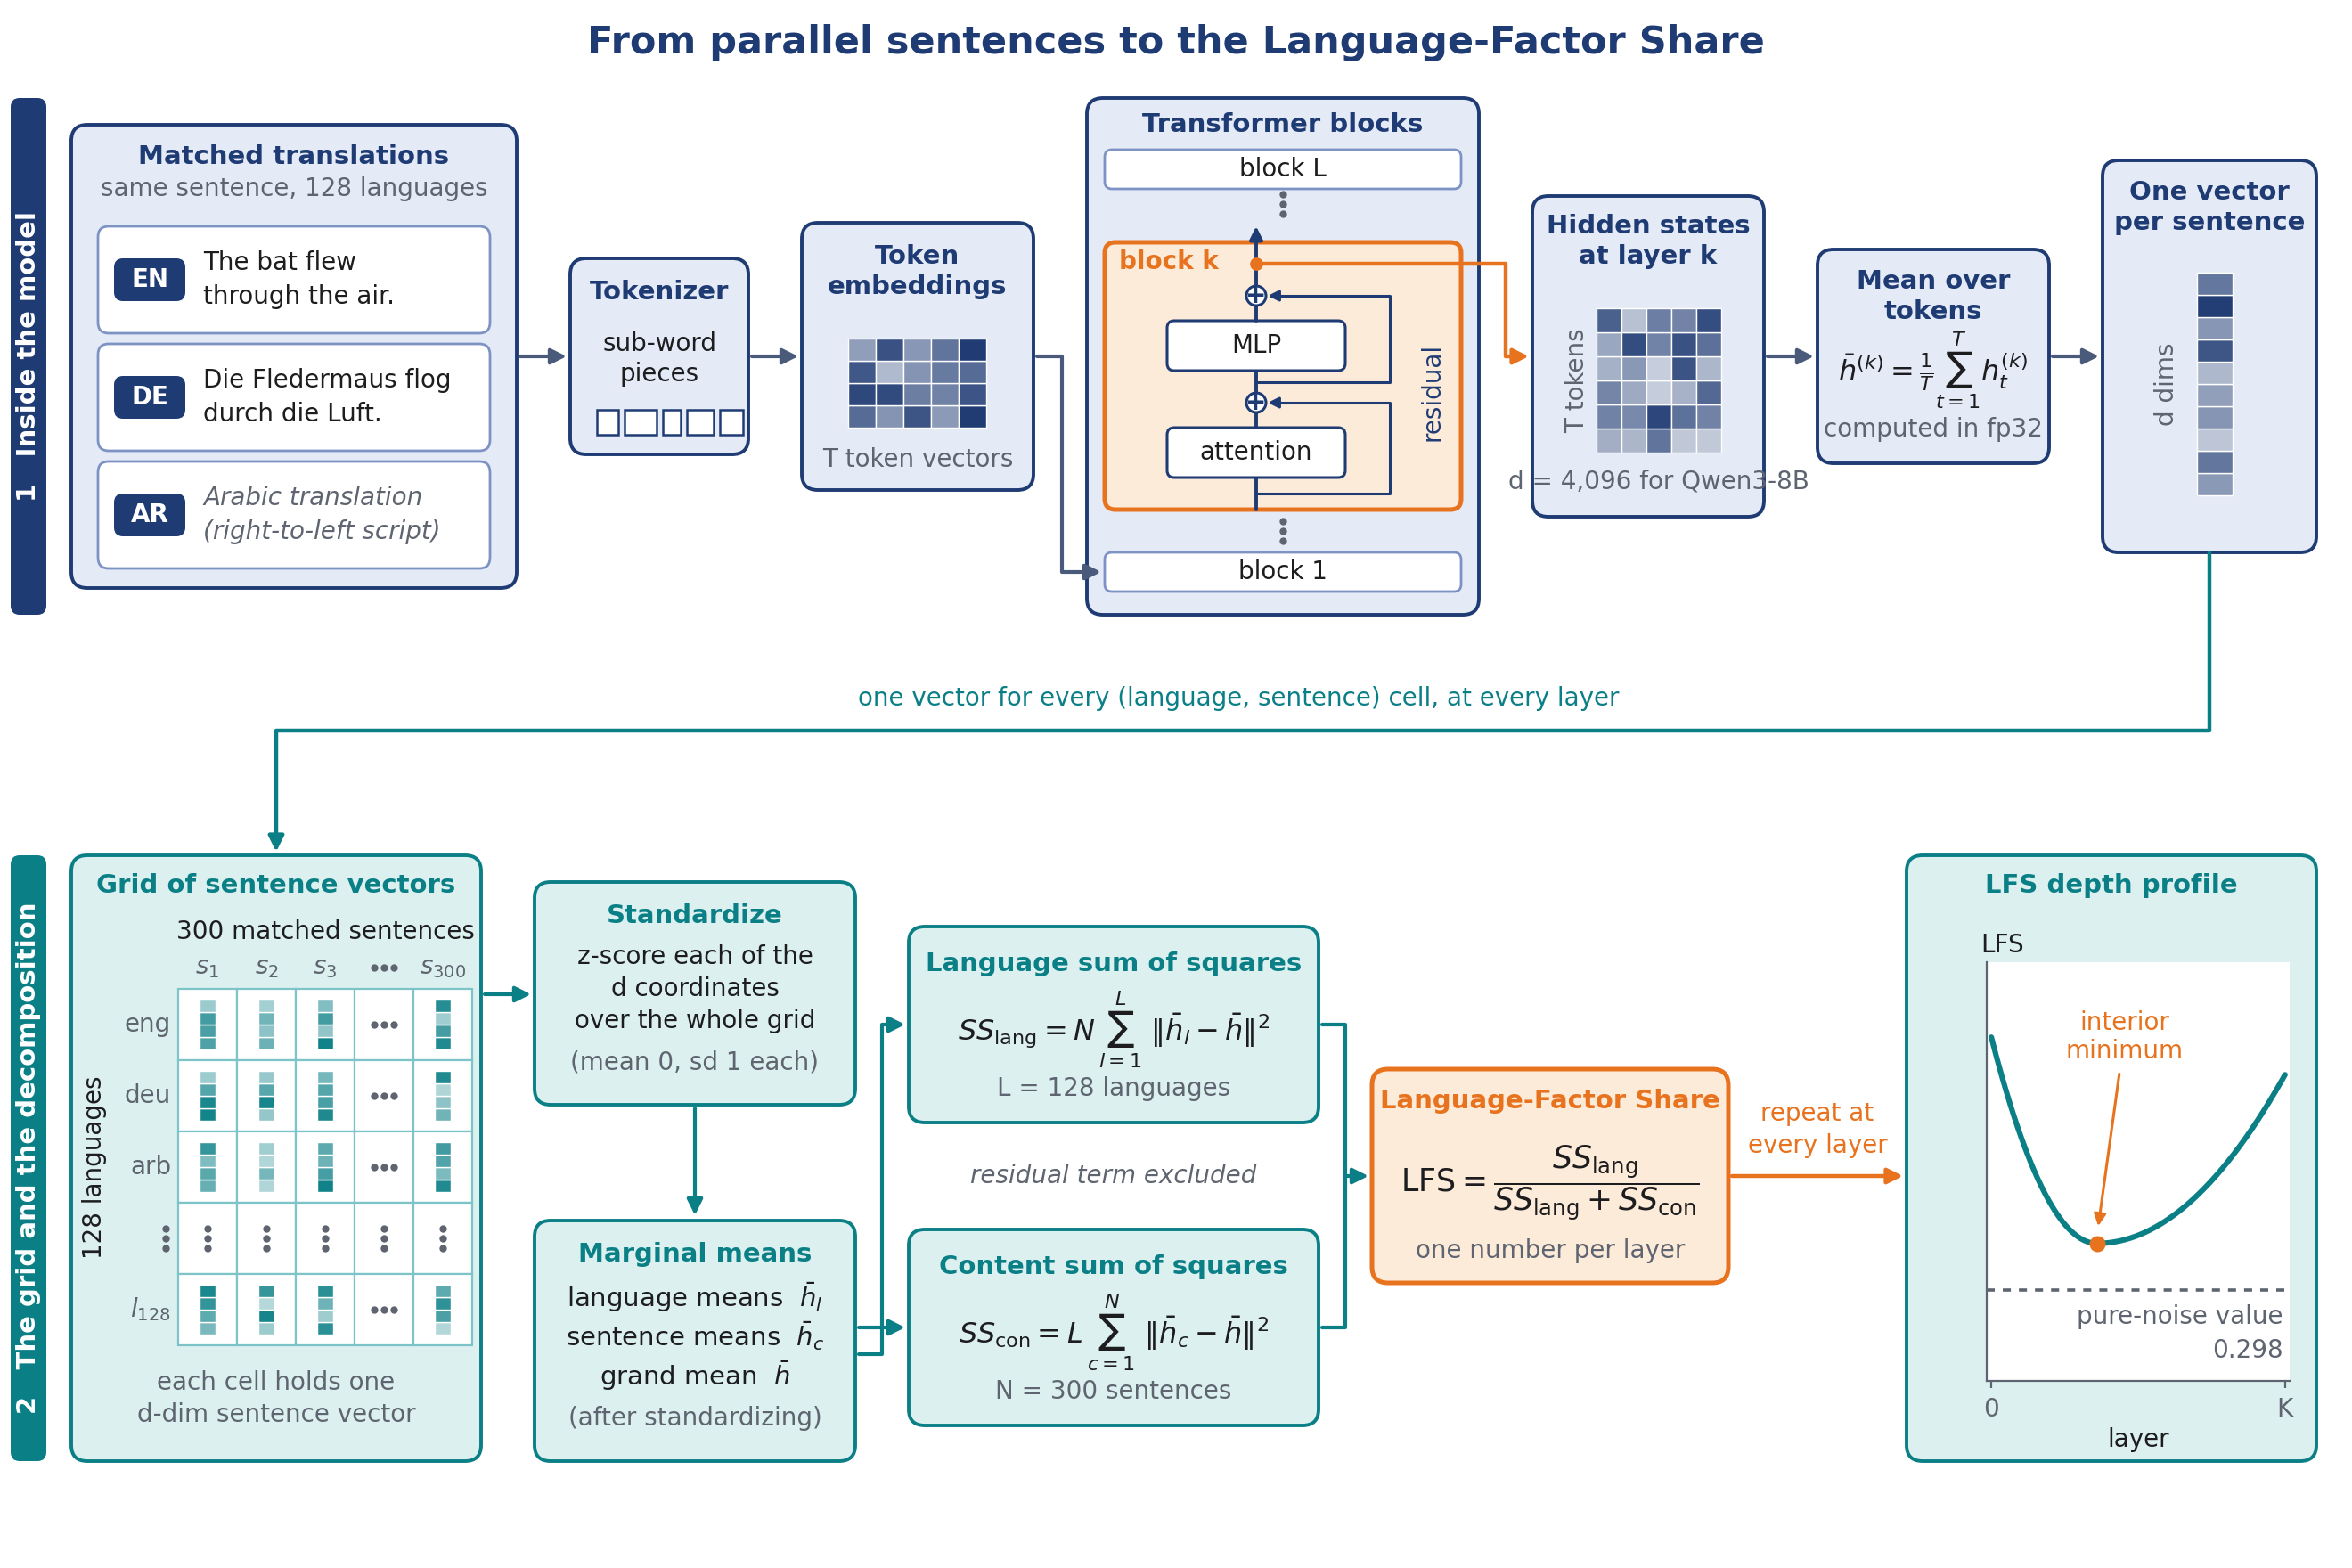
\includegraphics[width=\textwidth]{figs/fig22_pipeline_diagram.png}
  \caption{From parallel sentences to the Language-Factor Share. Top: inside
  the model, one sentence in each language is tokenized, embedded, and carried
  through the Transformer blocks; the hidden states at layer $k$ are averaged
  over tokens in fp32 into one vector per sentence. Bottom: the vectors of all
  128 languages and 300 matched sentences form a grid; each of the 4,096
  coordinates is standardized over the grid; language means, sentence means,
  and the grand mean give the two sums of squares, and their ratio is LFS at
  that layer. Repeating at every layer gives the depth profile.}
  \label{fig:pipeline}
\end{figure}

%==============================================================================
\section{Experimental Setup}
%==============================================================================
\subsection{Datasets}
\begin{itemize}
  \item \textbf{NTREX-128} \citep{federmann2022ntrex}: WMT newstest2019
  human-translated into 128 languages; $n$-way parallel through English.
  Primary text for all representation metrics (300 sentences; 500 for the
  hub-control run).
  \item \textbf{Belebele} \citep{bandarkar2024belebele}: 4-choice reading
  comprehension in 122 languages; our downstream target (300 questions per
  language, log-likelihood scoring via lm-evaluation-harness).
  \item \textbf{CulturaX} \citep{nguyen2023culturax}: per-language web-corpus
  token counts; the data-availability proxy (95 languages recovered;
  CC-100 sizes retained as a robustness alternative).
  \item \textbf{MEXA leaderboard + paper tables} (reference only): published MEXA scores for
  9 external models $\times$ 203 languages, parsed from the authors' LaTeX
  source; the external anchor grid.
  \item \textbf{Belebele metadata}: language family and script for all 122
  languages, grouped to Glottolog-style macro-families ($\geq 3$ members,
  else \emph{other}).
\end{itemize}

\subsection{Model grid}
Chosen to vary \emph{multilinguality by design} while providing within-family
scaling series (Table~\ref{tab:models}); all ungated base variants.

\begin{table}[H]
\centering
\small
\caption{The ten development-grid models. Unseen families (SmolLM2, Falcon3), the model kept out of the 1,500-sentence study (Salamandra 2B/7B), and the pre-registered additions (granite, Yi, Llama-3.1) are introduced in \S\ref{sec:walkforward} (the added families in its closing subsections), bringing the total evaluated to seventeen.}
\begin{tabular}{llllll}
\toprule
Model & Params & Layers & Developer & Training data & Runs on \\
\midrule
Qwen3 0.6B/1.7B/4B/8B & 0.6--8B & 28--36 & Alibaba & $\sim$36T tok, 119 langs & 2080Ti/A100 \\
OLMo-2 1B/7B & 1/7B & 16/32 & Allen AI & mostly EN, \emph{fully open} & 2080Ti/A100 \\
Mistral-7B-v0.3 & 7B & 32 & Mistral AI & EN/EU web & A100 \\
EuroLLM-1.7B & 1.7B & 24 & UTTER (EU) & $\sim$4T tok, 35 EU langs & 2080Ti \\
BLOOM 1.7B/7B & 1.7/7B & 24/30 & BigScience & ROOTS, 46 langs, \emph{open} & 2080Ti(fp32)/A100 \\
\bottomrule
\end{tabular}
\label{tab:models}
\end{table}

\textbf{Rationale.} Qwen3 = four-point scaling series under one recipe.
OLMo-2 = English-centric control with disclosed training data (exact token
counts for the confounder adjustment robustness subset). Mistral = independent 7B
EN-centric recipe. EuroLLM = \emph{targeted} multilinguality. BLOOM =
the multilingual-by-design archetype with open data; and the most
instructive model in the grid. EuroLLM-9B is gated and excluded;
$>$8B models enter only through the published MEXA anchor grid.

\subsection{Hardware and numerical precision}
Development and controls ran locally (Apple M5 Pro, 24\,GB, MPS); the grid on
the CLSP cluster: RTX 2080\,Ti nodes (fp16; fp32 for BLOOM-1.7B) and A100-80GB
nodes (bf16), scheduled as 1-GPU short-walltime jobs that backfill a saturated
partition efficiently ($\sim$55 minutes of total A100 time for the four large
representation runs). Three precision and protocol errors materially affected
results and are reported in \S\ref{sec:discipline}.

%==============================================================================
\section{Results I: The Representation Side}
%==============================================================================
\subsection{The LFS depth profile and what it reveals}
\begin{figure}[H]
  \centering
  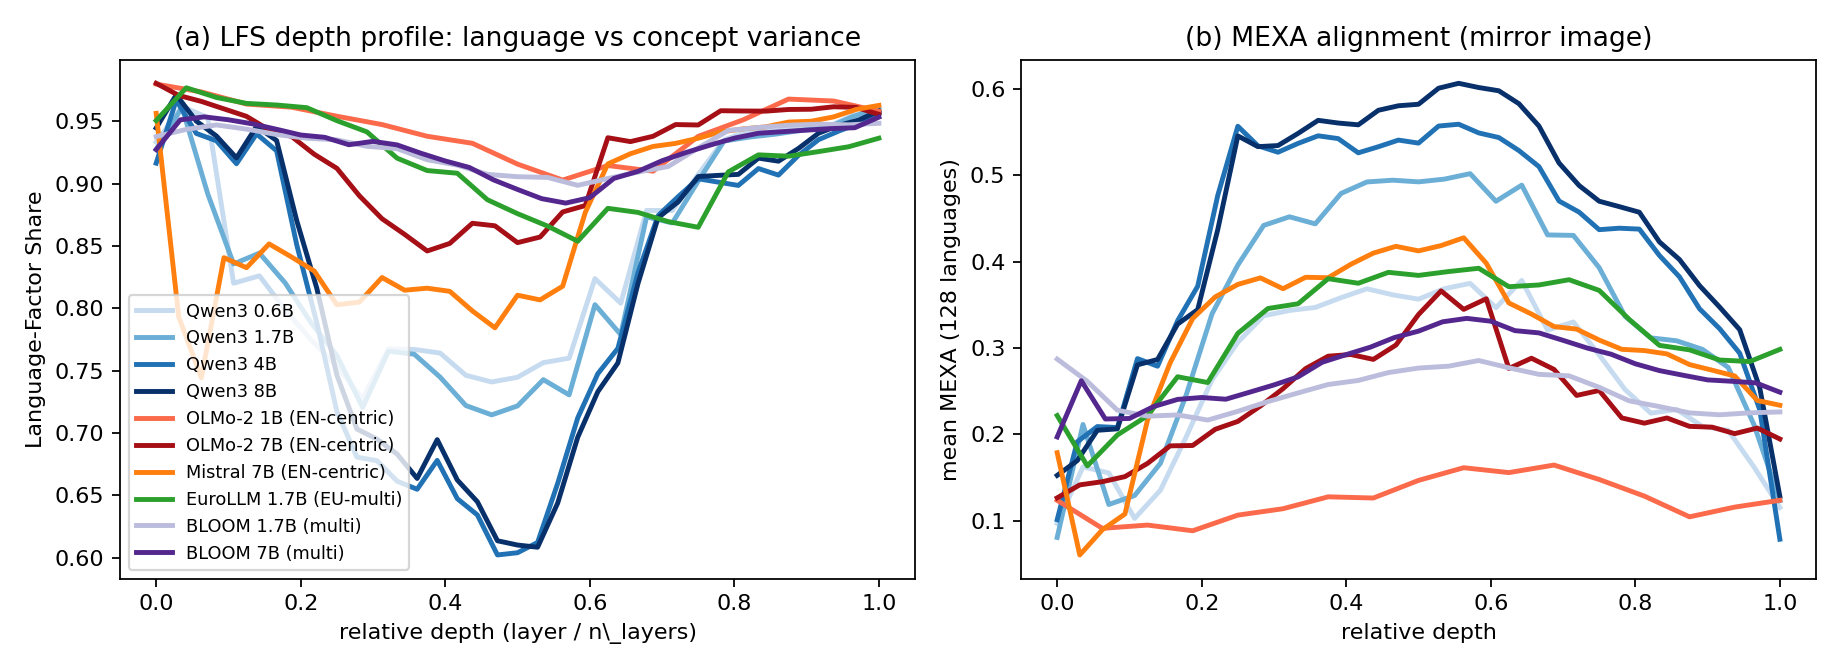
\includegraphics[width=\textwidth]{figs/fig1_lfs_depth_profile.png}
  \caption{(a) LFS by relative depth. Every model shows
  language-specific $\to$ shared $\to$ language-specific processing; the
  \emph{depth} of the concept dip varies from 0.04 (BLOOM) to 0.34 (Qwen3-8B).
  (b) Mean MEXA on the same grid, for reference: retrieval alignment peaks
  where the language share is lowest.}
  \label{fig:profile}
\end{figure}

\begin{figure}[H]
  \centering
  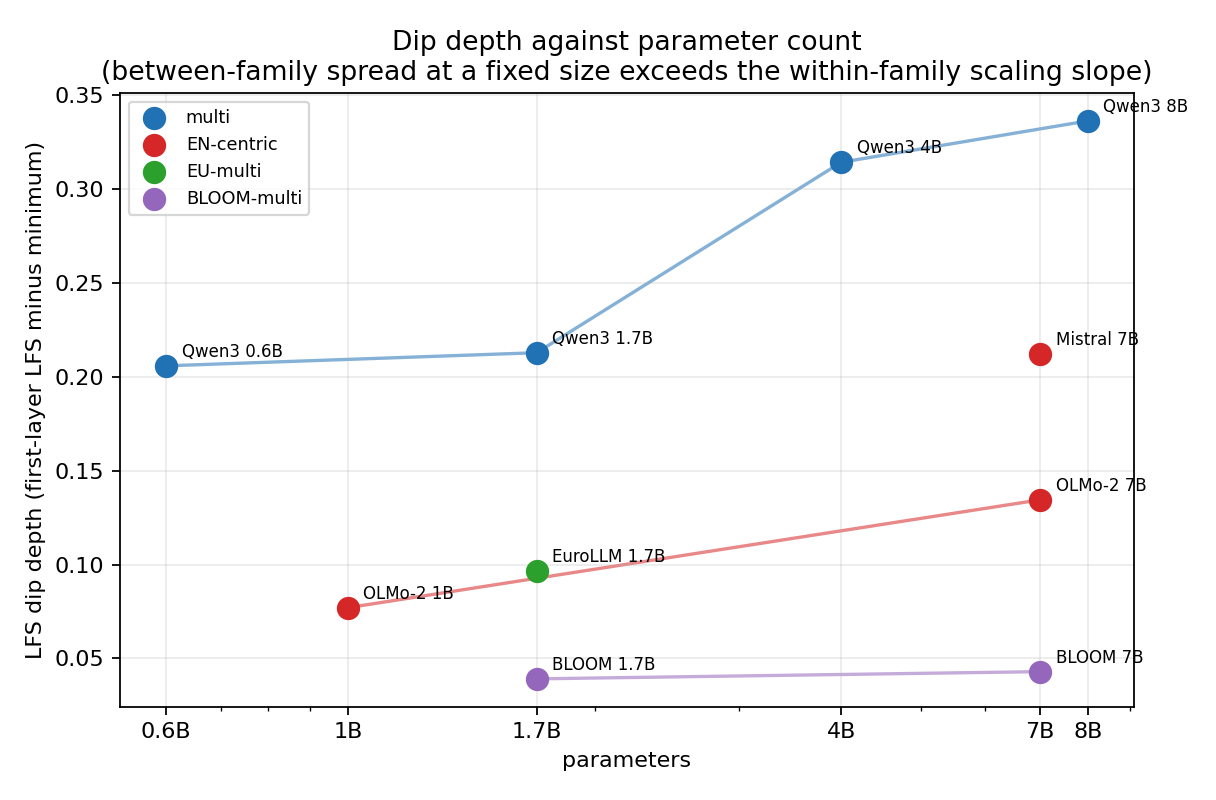
\includegraphics[width=0.72\textwidth]{figs/fig7_mix_vs_scale.png}
  \caption{Dip depth vs.\ parameters. Within-family lines slope upward
  (scale helps), but the vertical spread at fixed size dwarfs the slopes:
  \textbf{between-family differences dwarf within-family scaling}. Qwen3-1.7B
  (0.213) and Mistral-7B (0.212) are indistinguishable once sentence-bootstrap
  intervals are attached (\S\ref{sec:replication}).}
  \label{fig:mixscale}
\end{figure}

\begin{figure}[H]
  \centering
  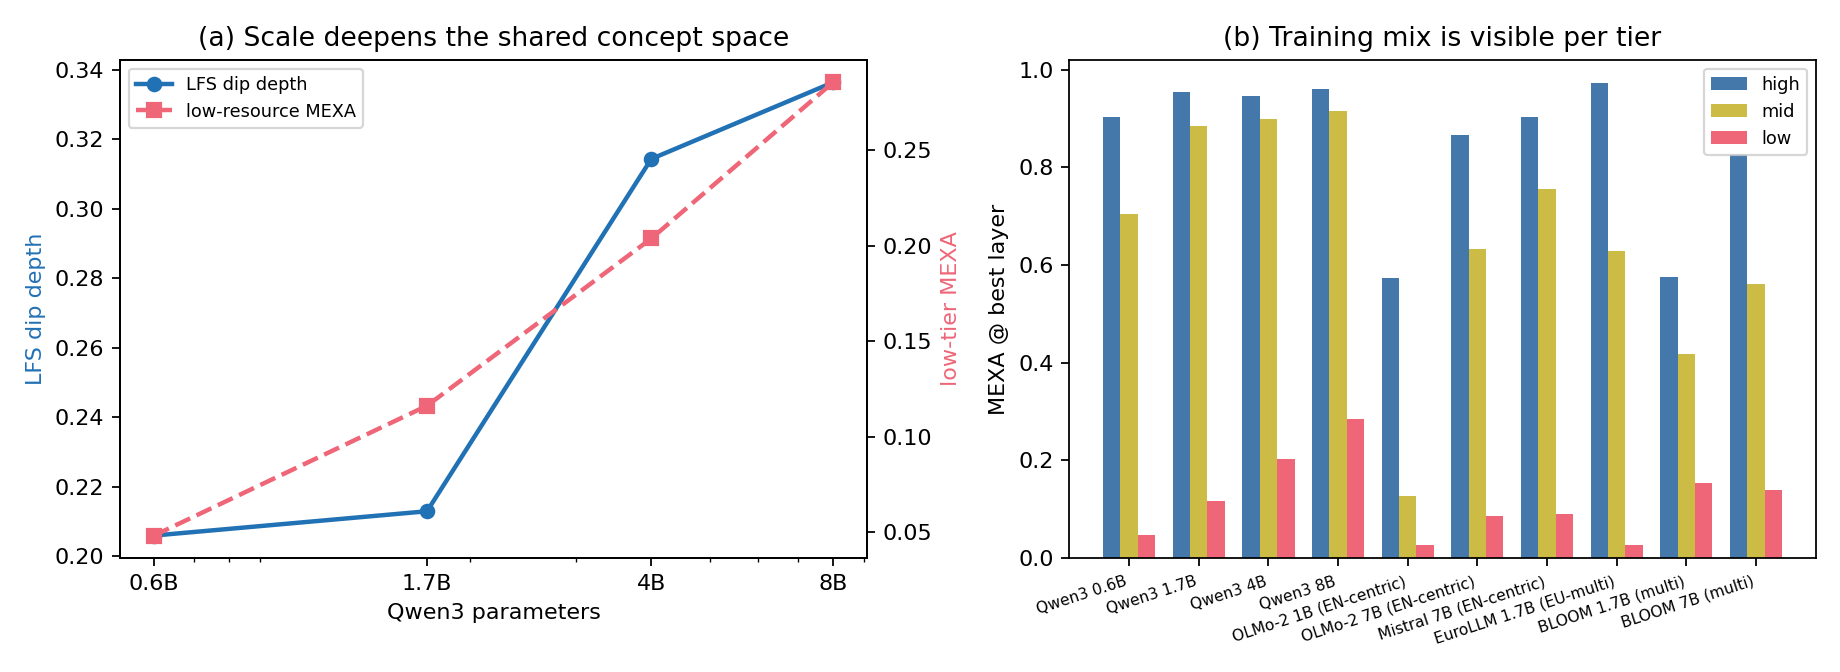
\includegraphics[width=\textwidth]{figs/fig2_scaling_tiers.png}
  \caption{(a) Qwen3 series: dip depth 0.206/0.213/0.314/0.336 and low-resource
  MEXA 0.048$\to$0.285 ($6\times$). (b) MEXA by resource tier at each model's
  best layer: OLMo-2 collapses outside high-resource; EuroLLM is near-ceiling
  on its EU targets (0.972) and near-floor elsewhere (0.028).}
  \label{fig:scaling}
\end{figure}

\begin{figure}[H]
  \centering
  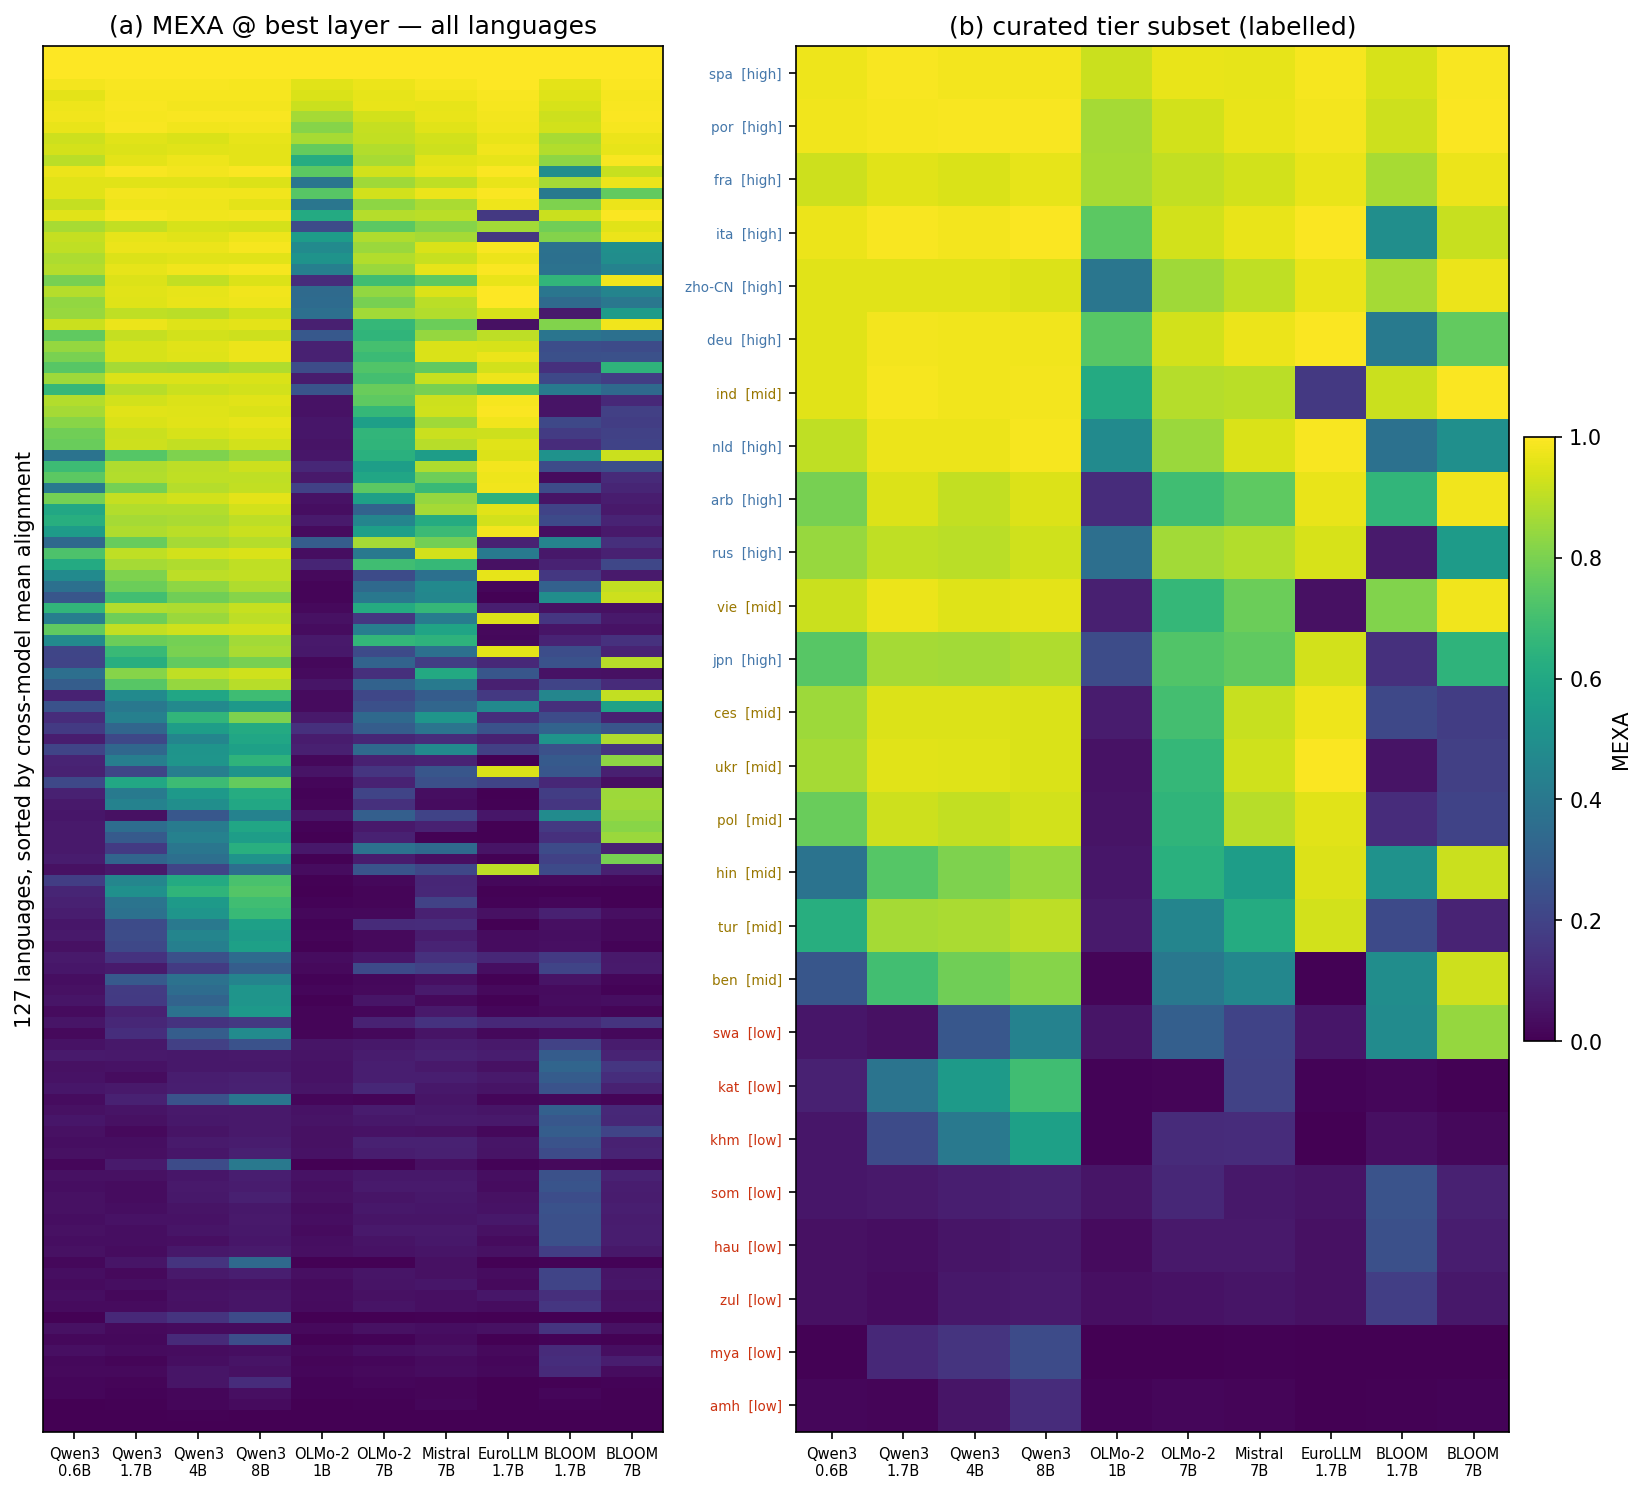
\includegraphics[width=\textwidth]{figs/fig6_heatmap.png}
  \caption{Reference measure: MEXA at best layer, languages $\times$ models. Column signatures:
  Qwen3 brightens and lengthens with scale; OLMo-2 dark outside the top band;
  EuroLLM bright exactly on its EU-35 block; BLOOM uniformly dim-but-nonzero.
  The bottom $\sim$30 rows are dark for \emph{every} model.}
  \label{fig:heatmap}
\end{figure}

\textbf{What ``recipe'' does and does not claim.} The claim that survives
scrutiny, stated precisely: between-family spread at fixed parameter count
dwarfs the within-family scaling slope. ``Recipe'' is deliberately a bundle; cross-lab comparisons confound data mix, total training tokens
(Qwen3's $\sim$36T vs.\ $\leq$5T elsewhere), tokenizer, and curriculum, and
these cannot be separated observationally (Mistral's 0.212 dip at ordinary
token budgets cuts against a pure token-count interpretation, but does not settle
it). The descriptive claim, not a causal decomposition, is what the Aim~2
argument requires: shared-space depth varies with training decisions far more
than with parameters, and the study shows it moves under direct optimization.

\textbf{Attribution of the U-shape.} The qualitative observation that
middle-layer representations are more cross-lingually similar predates this
work \citep{shani2025shared,wendler2024llamas}; our contribution is making the
dip depth a \emph{scalar} summary read against the estimator's null
value, which is shared by any two conditions measured at the same grid size
(\S\ref{sec:nsens}), and showing it varies by
almost an order of magnitude across models under mean pooling
(\S\ref{sec:pooling} measures how much of this depends on that choice)
(0.04--0.34 on the development
grid shown here; 0.37 including Llama-3.1, \S\ref{sec:walkforward}); large
enough to
serve as a model-selection and training signal.

\textbf{Coverage without convergence (BLOOM).} The only deliberately
balanced 46-language model has the \emph{flattest} LFS of all (dip 0.039 at
1.7B, 0.043 at 7B); flatter than English-centric OLMo-2, with alignment
concentrated at the embedding layer, direct evidence that what aligns is
surface form, not meaning. Its multilingual tokenizer aligns languages
\emph{lexically}; the transformer stack builds almost no shared concept
space, and a $4\times$ scale increase does not change that (a
script-disjoint LFS control to further isolate the tokenizer's contribution
is queued). One alternative interpretation is disclosed: both BLOOMs
($\sim$350B training tokens, 2022-era) are undertrained by modern standards,
so ``coverage without convergence'' could partly read as ``undertrained''; the 1.7B$\to$7B invariance does not rule this out, since both are
undertrained; separating the two requires a modern deliberately-balanced-mix
model, of which we are not aware in the open ecosystem. Coverage
is a data property; convergence is a training property; mean-level scores
see neither.

\subsection{Replication on a second corpus, sentence-level uncertainty, and instruction tuning (added 5 September 2026)}
\label{sec:replication}
Three checks were run under a protocol frozen before the jobs were submitted
(\texttt{prereg/addenda/AIM1\_EABC\_PROTOCOL\_2026-09-05.md}; CLSP jobs
1784646 to 1784649; scoring in \texttt{results/eabc\_scoring/}).
\textbf{FLORES-200.} Re-measuring all 17 primary-set models on FLORES-200
devtest (first 300 sentences; 116 of the 128 NTREX languages, English plus
115 of the 127 non-English languages, map to a FLORES code) reproduces the result: 17 of 17 profiles have an interior minimum
with both endpoints higher; dip depths agree with NTREX at Spearman 0.92 with a
median absolute difference of 0.011; the minimum layer agrees within two
layers for 14 of 17; and the per-layer profiles correlate at 0.94 to 1.00. The
three models whose minimum layer moved (Qwen3-0.6B, Mistral-7B, Salamandra-2B)
are the ones with a flat plateau or a very early minimum, where the argmin is
fragile although the curve is not. The largest depth change is granite
(0.190 on NTREX, 0.074 on FLORES). All five frozen predictions passed.
\textbf{Uncertainty.} Drawing 2,000 subsamples of 300 sentences from the
1,500-sentence 1,500-sentence dumps (identical index sets for every model) gives
95 percent intervals on dip depth with half-widths of 0.004 to 0.020 for 12 of
14 models and 0.045 and 0.059 for Mistral-7B and Salamandra-2B, the two
early-minimum models; the frozen half-width bar of 0.03 therefore fails for
those two and is reported as such. The cross-model ordering of dip depth is
consistent with the grid ordering at Spearman $\geq 0.90$ in 2,000 of 2,000 replicates (median $0.996$), and the first-300-sentence values used
throughout this report reproduce from the dumps to within $10^{-4}$. Random
subsets give slightly deeper dips than the first 300 sentences (by 0.004 to
0.06), so the main depths are conservative.
\textbf{Instruction tuning.} For six base and instruct pairs (Qwen3 0.6B,
1.7B, 4B, 8B; Qwen2.5-7B; Llama-3.1-8B) the profile is unchanged within 0.01
in dip depth, the minimum layer agrees within two layers for five of six, and
the final-layer share is higher for the instruct model in five of six pairs by
at most 0.003. The profile is a property of pretraining. All four frozen
predictions passed.

\subsection{The hub question: a multilingual latent factor, resource-graded, fading with scale}
With the
smoothness confound controlled ($N{=}500$ donor ranking), the latent factor
exceeds English for 113 to 124 of 127 languages depending on the model (124 for most), but modestly ($+0.08\,R^2$; our own
first estimate of $+1.04$ was $\sim$92\% confound; caught and corrected,
\S\ref{sec:discipline}). English is the best \emph{single} donor for 9/10
high-resource targets but 1/8 low-resource targets, where areal donors
(Indonesian, Hindi, Swahili) take over; across the Qwen3 series English's
best-donor share falls from 45/127 to 25/127. The common factor of better
models looks increasingly like a multilingual latent factor rather than
English; consistent with, though not yet proof of, an emerging
interlingua.

\subsection{Evaluation-size behaviour, and the estimator's null value}
\label{sec:nsens}
\begin{figure}[H]
  \centering
  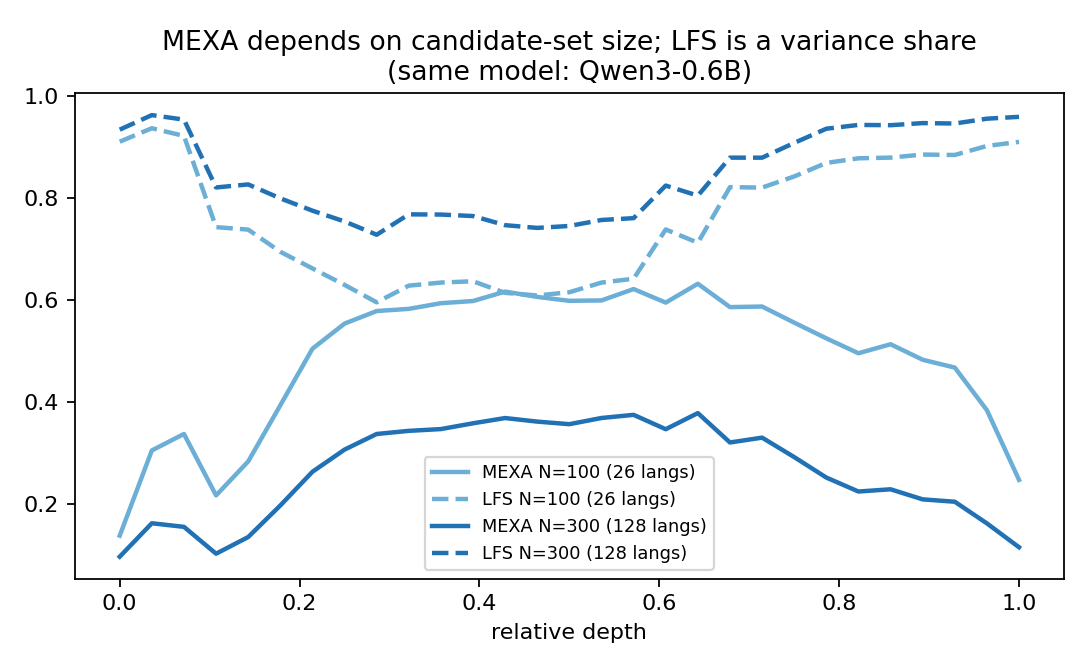
\includegraphics[width=0.62\textwidth]{figs/fig5_n_sensitivity.png}
  \caption{Same model, two evaluation sizes: MEXA drops 0.63$\to$0.38 from
  $N{=}100$ to $N{=}300$, because retrieval difficulty grows with the
  candidate set. Fairness note: MEXA's published protocol fixes $N{=}100$,
  so its own numbers are internally consistent; the sensitivity is a
  structural property of retrieval-based scores, not an execution flaw.
  The size behaviour of LFS is quantified directly below rather than
  asserted from its form.}
  \label{fig:nsens}
\end{figure}

\paragraph{The estimator's pure-noise value.} An earlier draft asserted
that variance shares are size-invariant by construction. That is very
nearly true but not exactly true, and the exact statement is more useful.
Writing the grid as $x_{c,\ell} = C_c + G_\ell + \varepsilon_{c,\ell}$ with
$\varepsilon$ independent of variance $\sigma^2$, the two sums of squares
expand as
\[
\mathrm{SS}_{\mathrm{lang}} = (L-1)D\sigma^2 + N\,\mathrm{SS}_G,
\qquad
\mathrm{SS}_{\mathrm{concept}} = (N-1)D\sigma^2 + L\,\mathrm{SS}_C ,
\]
so under a pure-noise null ($\mathrm{SS}_G = \mathrm{SS}_C = 0$) the
estimator returns the degrees-of-freedom ratio exactly:
\[
\mathrm{LFS}_{\mathrm{null}} \;=\; \frac{L-1}{(L-1) + (N-1)} .
\]
We verified this two ways. On synthetic noise it holds to within Monte
Carlo error across nine configurations spanning $L \in [2, 128]$,
$N \in [50, 3000]$, and $D \in [64, 1024]$, and it is independent of $D$
(\texttt{tests/test\_estimator\_floor.py}). On real saved representations,
a \emph{monolingual null}, in which one language's sentences are split into
disjoint groups relabelled as pseudo-languages so that neither true
language difference nor true concept correspondence exists, reproduces it
to three decimals: measured $0.0015$ against a predicted $0.00143$ at
$(L, N) = (2, 700)$, and $0.0849$ against $0.0846$ at $(12, 120)$, on all
four models tested.

Three consequences, in order of importance.

\emph{First, the measurement is not an artifact.} At matched $L$, $N$, and
$D$, real languages measure far above the monolingual null in every model:
at $(12, 120)$ the smallest real value exceeds the largest null value by
$0.15$ to $0.58$ depending on the model. The separation is positive in all
$20$ repeats of all four models.

\emph{Second, comparisons at a fixed grid share one null level.} The noise
term $(L-1)D\sigma^2$ enters the expectation of $\mathrm{SS}_L$ in the same
way for any two conditions measured at the same $L$ and $N$, so the
pure-noise value is a common reference for dip depth, for cross-model
comparison on a fixed language set, and for before-and-after injection
contrasts. It does not cancel: a difference of two ratios that both carry the
term is not free of it, and the expressions above are expectations under the
stated assumptions, not identities for an observed sample. Every comparative
claim in this report is therefore read against the shared null, not net of
it.

\emph{Third, absolute values are not comparable across grids, and a small
LFS is not by itself evidence of language-agnosticism.} The pure-noise
value is $0.298$ at the development grid $(128, 300)$ and $0.078$ at the
1,500-sentence grid $(128, 1500)$; absolute LFS values from the two should not be
placed side by side. And because the numerator carries a noise term that
does not vanish, a model approaching true language-agnosticism does not
drive LFS to zero. It approaches a value set by the residual scale. This
bears directly on Aim~2: an objective that minimizes LFS is pushing against
an asymptote, not toward zero, which is one more reason the target must be
constrained rather than minimized.

Note also that the pure-noise value is not a lower bound. A grid with
strong concept structure and weak language structure measures below it,
because $L\,\mathrm{SS}_C$ grows while the numerator's noise term does not;
this is verified in the same test file.

\paragraph{Measured size dependence on real data.} On the 1,500-sentence
representations with a fixed 12-language set and nested sentence samples
(twenty repeats per size), LFS moves by $-0.006$ to $-0.010$ from
$N{=}100$ to $N{=}1000$, while mean MEXA moves by $-0.065$ to $-0.125$ on
the same draws: a factor of ten to nineteen. The small negative LFS drift
is in the direction the expansion predicts, since the noise term's share of
the numerator shrinks as $N$ grows. The practical claim is therefore that
LFS is \emph{nearly} size-invariant with an analytically characterized
residual dependence, and that retrieval-based scores are not.

Honesty requires the symmetric statement: \textbf{the size-invariance
argument accrues to LFS alone}. AaR@10 is itself retrieval-based and inherits
the same candidate-set sensitivity, so its values are comparable only within
a fixed protocol ($N{=}300$ throughout). A related caveat: with 300 sentences per language, each language's
worst decile is 30 sentences, so \emph{per-language} AaR estimates are noisy; cross-language and cross-model aggregates are the reliable objects.

%==============================================================================
\section{Results II: Downstream Attribution and Confounder Adjustment}
%==============================================================================
\subsection{Protocol}
Belebele, 0-shot, log-likelihood scoring, 300 questions per language,
identical for all models. The uniform 0-shot choice is forced and disclosed:
5-shot prompts ($\approx$8.4k tokens) silently exceed short context windows; BLOOM (2,048) lost the passage entirely and scored \emph{below chance} on
English; OLMo-2/EuroLLM (4,096) silently degraded to $\sim$2-shot. Uniformity
of the benchmark is non-negotiable for attribution; the 5-shot runs are retained
as a robustness set for long-context models only.

\subsection{The validity check, the coefficients, the adjustment}
The advisor-specified validity check; the data-availability beta must be
positive and significant, else every residual downstream is meaningless; passes decisively:
\[
\beta(\log_{10}\text{tokens}) = +0.286 \;\; (\mathrm{SE}\ 0.059,\ z = 4.8),
\qquad R^2 = 0.824 \quad (17\text{-model grid}, n = 1{,}241).
\]
(The 10-model development grid gave $+0.267$, SE $0.051$, $R^2 = 0.86$; see the discrepancy ledger, D13.)
Fertility carries the predicted negative sign ($\beta = -0.103$, SE $0.022$):
the tokenizer tax is real. With the benchmark and the factors in place,
Figure~\ref{fig:deflation} shows the central result.

\begin{figure}[H]
  \centering
  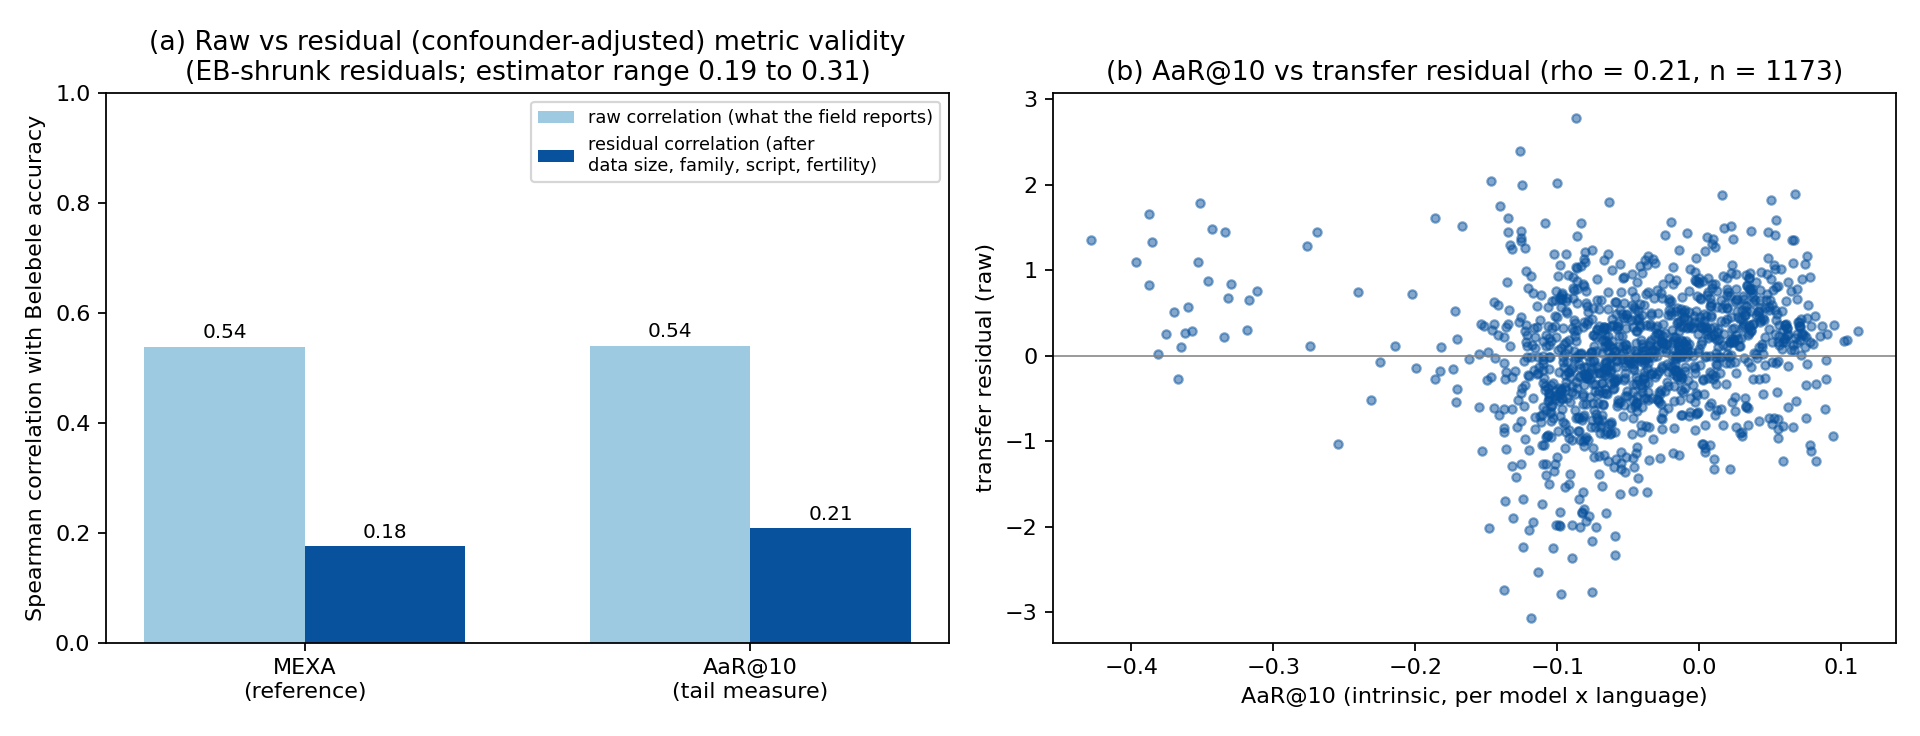
\includegraphics[width=\textwidth]{figs/fig8_deflation.png}
  \caption{(a) Raw vs.\ residual (residual) correlations for the tail measure
  AaR@10 and, for reference, MEXA (raw-residual estimator shown; the scheme
  range is 0.19--0.31, \S\ref{sec:hardening}a). The surviving residual signal
  is real; the two measures are not ranked on it (Appendix~\ref{app:compar}).
  (b) AaR vs.\ raw transfer residual across (model, language) pairs.}
  \label{fig:deflation}
\end{figure}

\begin{table}[H]
\centering
\small
\caption{Metric validity, raw vs.\ confounder-adjusted (development grid: 10 models $\times$ 122
languages, 0-shot Belebele). Spearman correlations; all individually survive
Benjamini--Hochberg correction. The residual level depends on the estimator
(the estimator range, \S\ref{sec:hardening}a). MEXA is shown for reference
and the two rows are not ranked (Appendix~\ref{app:compar}).}
\begin{tabular}{lccc}
\toprule
 & vs.\ raw acc. & vs.\ residual (raw) & vs.\ residual (within-family) \\
\midrule
AaR@10 (tail measure) & 0.50 & 0.23 & 0.25 \\
MEXA (reference) & 0.53 & 0.19 & 0.27 \\
\bottomrule
\multicolumn{4}{l}{\footnotesize Median-$s^2$ disattenuation gives
0.27 (MEXA) / 0.31 (AaR); the EB point estimates of an earlier draft are
withdrawn (\S\ref{sec:hardening}a).}\\
\end{tabular}
\label{tab:deflation}
\end{table}

\begin{figure}[H]
  \centering
  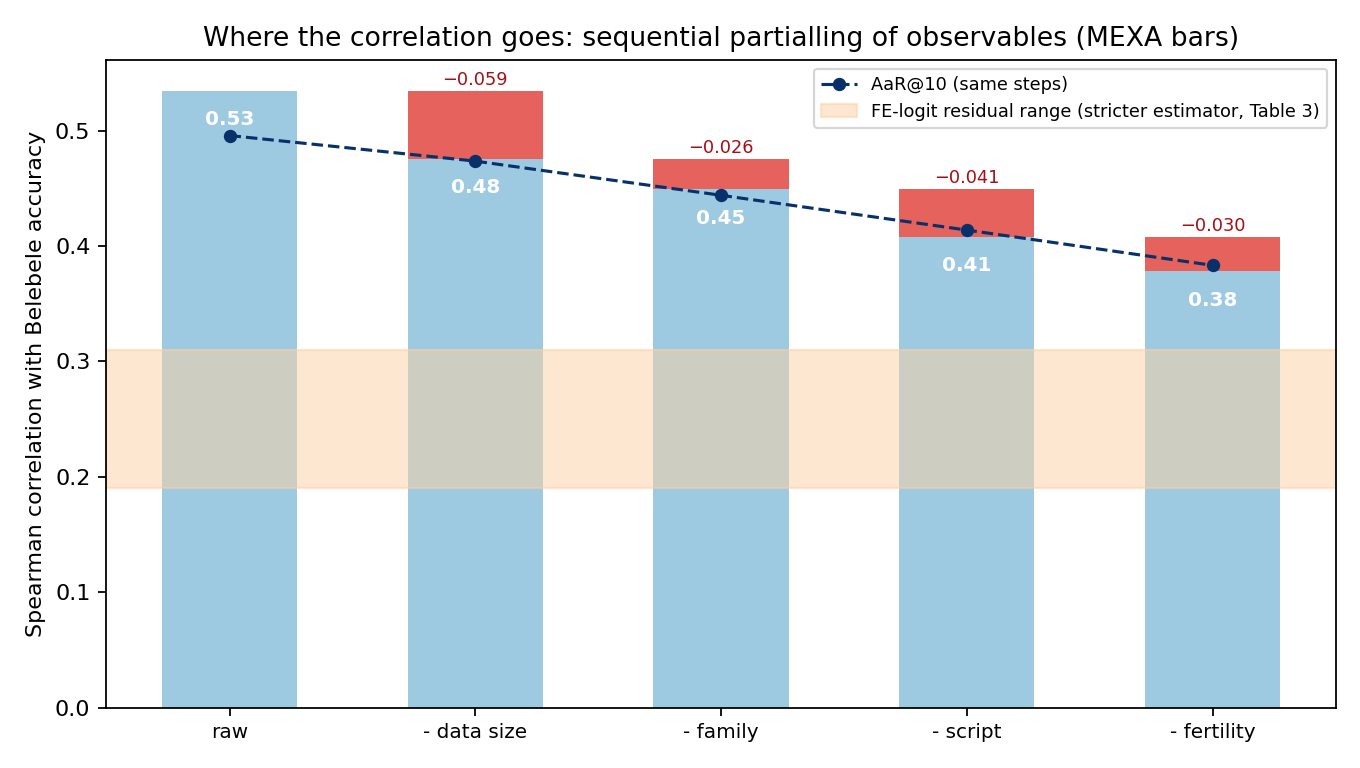
\includegraphics[width=0.78\textwidth]{figs/fig11_waterfall.png}
  \caption{``Most of the raw correlation is exposure,'' as one picture: sequential
  rank-partialling of observables out of the metric--accuracy correlation
  (order as shown; order-dependence disclosed). The chart's endpoint is
  the partial-Spearman estimator; the shaded band is the stricter FE-logit
  residual range of Table~\ref{tab:deflation}; together they bound the
  confounder adjustment.}
  \label{fig:waterfall}
\end{figure}

\paragraph{The refresh at 17 models, and a withdrawn subset figure.} After the pre-registered family additions
(\S\ref{sec:newfam}), the attribution refresh runs on 17 models (1{,}173
fitted rows). The all-model range \emph{holds} (raw $\rho \approx 0.54$;
residual $\rho \approx 0.18$--$0.21$); and the structure behind it is now
measured rather than conjectured: the models diluting the pooled number are
the chance-floor ones, which have no downstream variance for \emph{any}
metric to predict. On the \textbf{benchmark-capable subset under the frozen criterion (aggregate
accuracy $\ge 0.30$: ten models, six independent families)}, the July
analysis reported a confounder-adjusted correlation of about $0.59$ ($n = 690$) that
survived deleting the Qwen3 family ($0.53$). \textbf{That figure is not
reproducible from any stored artifact.} A re-derivation on the current
stack with the same rule gives $0.487$ $[0.365, 0.554]$ for retrieval
alignment at the LFS-selected layer (discrepancy ledger, 2026-08-05), and
the cause of the gap (estimator scheme, residual shrinkage, or language set)
is undetermined. The conservative all-model range is therefore the only
benchmark-target number this report stands on; the benchmark-capable figure is
withdrawn until it can be regenerated from a manifest. The frozen criterion
was applied against convenience both ways: SmolLM2 ($0.283$) and
Salamandra-7B ($0.2945$) sit just under the bar and stay excluded.

\subsection{Statistical hardening}
\label{sec:hardening}
Four adversarially-motivated checks, all on existing data:

\textbf{(a) Shrinkage, in three steps; and the estimator range.}
\emph{Step 1:} our first shrinkage implementation reduced to weights of
$(n{-}1)/n$ (shrinkage in name only); correlations against those
effectively-raw alphas (MEXA 0.19, AaR 0.23) are attenuated by sampling noise.
\emph{Step 2:} correct-looking empirical-Bayes weights
($\tau^2/(\tau^2+s_i^2)$) roughly doubled both correlations (0.41/0.43); but diagnostics revealed a new artifact: the logit derivative explodes for
chance-floor rows ($s_i^2$ up to $\sim$6 logits$^2$ at the clip boundary),
dragging every family's $\hat\tau^2$ \emph{negative} and collapsing the median
weight to $3\times10^{-4}$. The ``shrunk alphas'' were $\sim$99.9\%
macro-family means, so the doubled correlations largely measured
metric-vs-family structure, with effective sample size closer to
(families $\times$ models) than to $n{=}690$. Those numbers are withdrawn.
\emph{Step 3:} scheme-robust estimates. Family-demeaning both metric and raw
residual (which shrinkage cannot flatter) gives AaR 0.25 / MEXA 0.27;
median-$s^2$ disattenuation (reliability 0.52, no routing through family
means) gives AaR 0.31 / MEXA 0.27. \textbf{The defensible statement:
intrinsic metrics correlate with transfer residual at $\rho \approx 0.19$--$0.31$
depending on estimator (vs.\ 0.50--0.53 raw), i.e., an confounder adjustment of
roughly 40--60\%, with every estimator's failure mode documented.} The
confounder adjustment methodology is what makes the range, rather than a
confidently wrong point estimate, possible.

\textbf{(b) Two measures on one target.} Whether the tail measure and
MEXA differ in confounder-adjusted validity was tested by cluster bootstrap on
$\Delta\rho$ under each estimator scheme; the difference is not scheme-stable
and the analysis is recorded, unchanged, in Appendix~\ref{app:compar}. The
claim this report stands behind is narrower: \textbf{the tail measure
exposes failures that mean-level measures cannot represent}
(\S\ref{sec:boundary}); its confounder-adjusted validity is reported above without
ranking. Model-level dependence cannot be cleanly resampled with 10 model
clusters; language-cluster bootstrap is the primary specification;
acknowledged, not solved.

\textbf{(c) Floor robustness $=$ clipping robustness.} The logit clip at 0.26
piles exactly the chance-floor rows at the boundary, so the drop-floor refit
doubles as the clipping-sensitivity check: on the six benchmark-capable models the
gate strengthens ($\beta_{\mathrm{tokens}} = +0.359$, $p = 1.3\times10^{-6}$;
fertility $-0.34$, $p<0.001$), and the residual correlations persist
(AaR 0.30, MEXA 0.26).

\textbf{(d) Layer-selection sensitivity.} The ``best layer'' rule (argmax
mean MEXA) was chosen on this grid, so we recomputed validity at a fixed
relative depth of 0.5: MEXA is essentially unchanged (raw $0.535 \to 0.503$;
residual $0.194 \to 0.181$) and AaR attenuates but persists (raw
$0.496 \to 0.363$; residual $0.226 \to 0.168$). The results do not ride on the
layer-selection rule; AaR's larger sensitivity (tail margins move more across
layers) is noted.

\textbf{(e) Family-dropout and matched-pairs checks.} Leave-one-family-out:
six of seven exclusions leave the residual correlations stable (0.18--0.33);
excluding \textbf{Qwen3} collapses them to 0.06/0.09. Our interpretation, labeled as interpretation, is floor contamination: without the one fully
benchmark-capable scaling family, most remaining rows sit at the chance boundary
where the residual has little variance (Falcon3's held-out 0.66 cuts against pure
Qwen3-specificity), but the dependence is disclosed as a fact; additional
capable multilingual families are the remedy. The factor-neutral
counterweight: within $\sim$800 language pairs matched on macro-family,
script, and data size ($|\Delta \log \mathrm{tokens}| < 0.75$), the
higher-metric language has higher residual 59--60\% of the time
(binomial $p < 10^{-5}$ for both metrics); the metric separates even
matched languages.

\textbf{(f) The chance-floor models fail the benchmark, not the languages.}
EuroLLM-1.7B scores 0.250 on ten high-resource European languages, its own
target languages, where its alignment is 0.97, while the size-matched
control Qwen3-1.7B scores 0.685 on the same set. BLOOM-1.7B/7B likewise
(0.248/0.234). This is capability/format failure at 0-shot multiple choice,
not alignment failure; ``alignment is necessary but not sufficient'' is
accordingly stated at the capability level, and the confounder adjustment results are
reported with and without these models.

\subsection{Mean-versus-tail downstream scoreboard}
\begin{figure}[H]
  \centering
  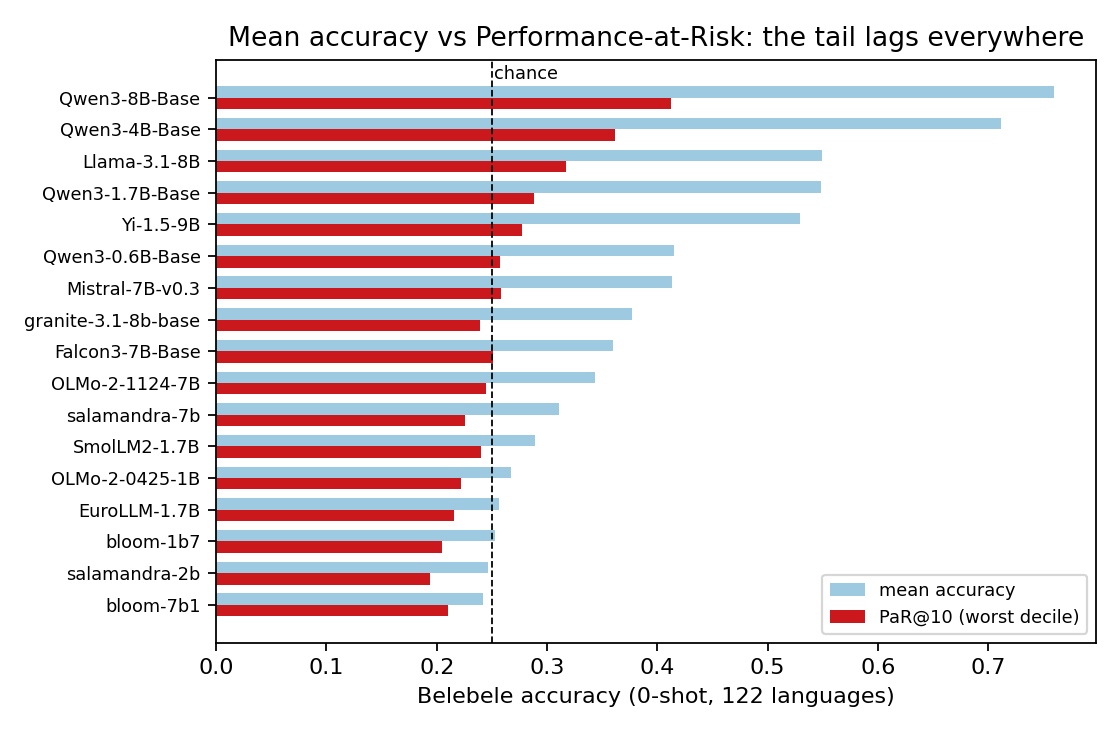
\includegraphics[width=0.7\textwidth]{figs/fig9_par.png}
  \caption{Mean accuracy vs.\ Performance-at-Risk (worst decile of languages).
  The tail lags everywhere; several models' tails sit at the chance line
  their means comfortably clear.}
  \label{fig:par}
\end{figure}

\begin{figure}[H]
  \centering
  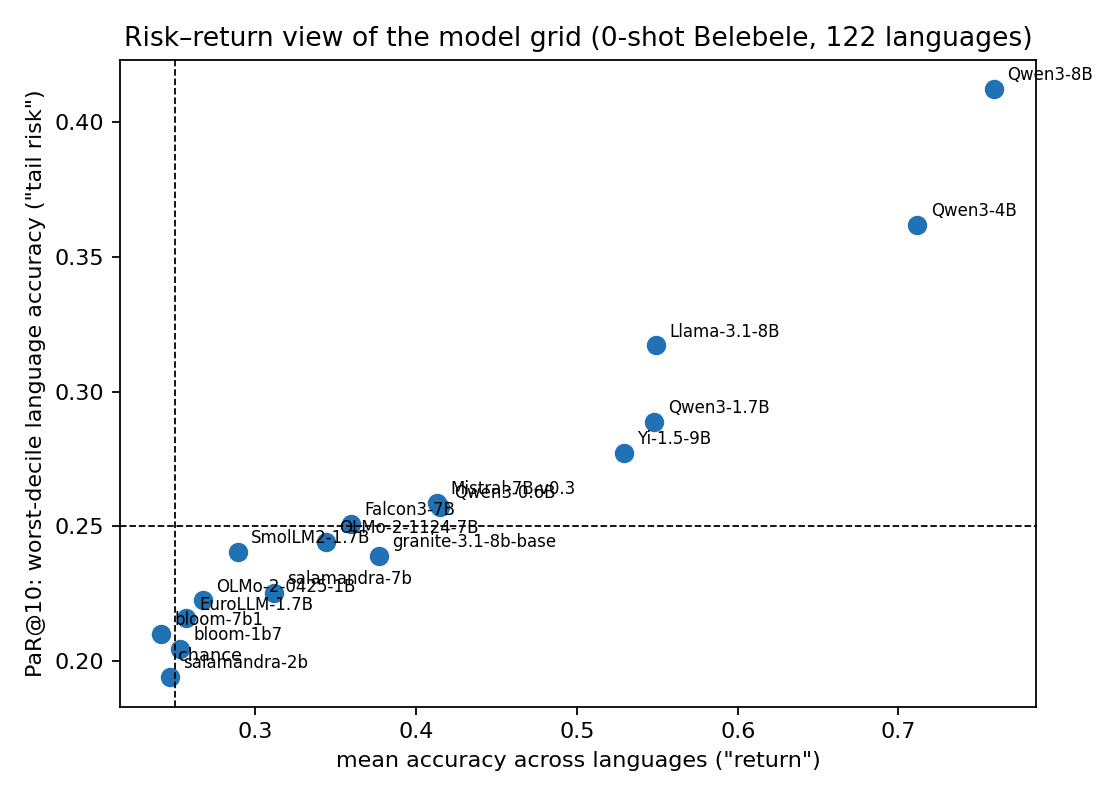
\includegraphics[width=0.62\textwidth]{figs/fig13_riskreturn.png}
  \caption{Mean-versus-tail view of the grid: mean accuracy (``return'') vs.\
  worst-decile language accuracy (``the tail''). Dominance is immediate:
  Qwen3-8B dominates on both axes; the chance-floor cluster sits in the
  bottom-left corner.}
  \label{fig:riskreturn}
\end{figure}

Two details the mean-versus-tail view shows. First, \textbf{EuroLLM-1.7B}: near-ceiling
\emph{alignment} on EU languages but chance-level Belebele accuracy; and the
own-turf probe (\S\ref{sec:hardening}f) shows this is 0-shot benchmark incapacity
rather than language incapacity: alignment is necessary but not sufficient for
\emph{measured} task capability. Second,
the naive per-model ``total residual'' is zero by construction under model fixed
effects, and the FE-residual tail residual measures \emph{headroom collapse}
(strong models fall furthest below their own level at the data-poorest
decile) rather than tail service; \textbf{PaR@10} is the correct
``who serves the tail'' statistic, and Qwen3-8B leads it (0.412).

\subsection{What is actually in the tail?}
We read the worst-decile sentences (Qwen3-0.6B, best layer) for Hindi,
Turkish, Bengali, and Vietnamese. The prior worry; that NTREX news text
would make the tail a named-entity/transliteration artifact; is refuted by
the data, in an instructive direction: \emph{entity- and numeral-dense
sentences populate the best-aligned end} (``CBS had 3.1 million, NBC had 2.94
million\ldots'' attains the top margin in multiple languages; names and digits
act as cross-script anchors). The tail instead consists of
(i)~\textbf{discourse-dependent, semantically light sentences}; ``Interest remained high after the hearing.'' (margin $-0.135$, Hindi): seven
ordinary words whose interpretation hangs on an unresolved anaphor;
(ii)~\textbf{culturally specific institutional vocabulary} (parish
vestry/diocese disputes, Welsh-Assembly terminology); and
(iii)~\textbf{news boilerplate crowded by near-duplicate decoys} (``Police
have urged people\ldots to come forward''), where low margins partly reflect
a property of the decoy set rather than of the language. Several sentences
recur in the worst decile of multiple languages; tail difficulty is partly
sentence-intrinsic. Net: AaR is measuring the loss of \emph{fine-grained
semantic} alignment, exactly the failure mode that matters for downstream
use, with a corpus-crowding component we disclose rather than hide.

%==============================================================================
\section{Confirmation Experiments: \S3.1.2 and \S3.1.3, Pre-Registered}
%==============================================================================
\label{sec:confirm}
The proposal's two remaining Aim-1 subsections were executed as
\emph{pre-registered confirmation tests} of the metric findings: all
predictions were derived from the already-computed grid results and frozen in
\texttt{PREREG\_312\_313.md} before any run (round 1: A1--A4, B1--B4; round 2,
after documented round-1 lessons: A2$'$, B2$'$, B4$'$, B5). Combined tally:
\textbf{9 of 13 predictions passed; every failure is reported and produced
either a new finding, a corrected mechanism, or a methodology lesson.}

\paragraph{Experiment A; corrected lens probe (\S3.1.2).}
Per-layer states of non-Latin-script inputs are projected through the output
vocabulary; token script is classified by Unicode block.
\emph{Passed:} every Qwen3 model shows an interior valley in input-script
mass (A1); mid-layer Latin dominance shrinks with scale, $0.34 \to 0.23$ from
0.6B to 4B (A3; non-monotone at 1.7B, disclosed); and the proposal's concern
about Logit Lens is quantified (A4): hidden states reach a maximum cosine of
only $\sim$0.10 to \emph{any} output embedding in the very layers the lens
literature interprets ($\sim$0.20 at the final layer); raw lens conclusions
about middle layers are weakly supported by the geometry, as \S3.1.2 of the
proposal suspected.
\emph{Failed; and recorded as a finding:} the lens valley does
\textbf{not} coincide with the LFS dip (A2; only the 0.6B coincided).
The round-2 matched-pooling rerun (A2$'$) confirms the gap persists in all
four models (0.18--0.56 relative depth): \textbf{the multilingual depth profile has
two distinct events}; surface-script abandonment early ($\sim$0.05--0.19
depth), concept-variance convergence mid ($\sim$0.3--0.5). Neither instrument
alone would have revealed this.

\paragraph{Experiment B; cross-lingual context transfer (\S3.1.3).}
Adjacent same-document NTREX pairs; the target sentence is always English,
the context sentence varies over languages; benefit is the target's NLL
reduction. Round 1 (13 languages) passed the direction tests (context is
used, B1; benefit grows with scale $0.16 \to 0.35 \to 0.43$, B3) but failed
the underpowered correlation bar (B2: $\rho = +0.31$ vs.\ a pre-registered
0.5 at $n{=}12$, a threshold set without power analysis, our error).
Round 2 added the decisive control, \emph{mismatched context} (same
language, wrong document); and 40 context languages:

\begin{table}[H]
\centering
\small
\caption{Round 2 (B2$'$): Spearman correlation between per-language intrinsic
alignment (MEXA at best layer) and content-specific context benefit
$R_{\mathrm{content}}$ (matched $-$ mismatched, normalized to English),
$n{=}40$ languages.}
\begin{tabular}{lcc}
\toprule
Model & $\rho$(alignment, $R_{\mathrm{content}}$) & $p$ \\
\midrule
Qwen3-0.6B & 0.958 & $<10^{-13}$ \\
Qwen3-1.7B & 0.938 & $<10^{-13}$ \\
Qwen3-4B & 0.883 & $<10^{-13}$ \\
OLMo-2-1B & 0.882 & $<10^{-13}$ \\
\bottomrule
\end{tabular}
\label{tab:b2prime}
\end{table}

The raw correlations in Table~\ref{tab:b2prime} clear the pre-registered bar
($\rho \geq 0.35$, $p<0.05$) by a wide margin; but our own \S6 forbids
taking a raw intrinsic$\leftrightarrow$outcome correlation at face value:
alignment and context benefit are both monotone in per-language competence,
which is itself resource-driven. So we applied the paper's confounder adjustment
machinery to this validation target too, partialling log tokens,
macro-family, script, and fertility out of \emph{both} variables.
\textbf{The confounder-adjusted result: alignment predicts content-specific context
benefit beyond what observables predict; pooled residual Spearman
$+0.67$; per model $+0.77$/$+0.28$/$+0.60$/$+0.71$} (the weak 1.7B cell,
$p{=}0.09$, disclosed; Figure~\ref{fig:b2scatter}). Because the 152 pooled
rows repeat 38 languages across four models, the na\"ive $p$ overstates the
evidence; with language-cluster bootstrap the CI95 is $[0.55, 0.77]$, and the
most conservative treatment, averaging residuals per language so each of
the 38 languages is one independent unit, still gives $\rho = 0.46$,
$p = 0.004$. The claim survives at every level of strictness. Content transfer is positive for 100\% of the
40 languages in Qwen3-4B (B5(ii)); OLMo-2's non-European-script content
transfer is under half of Qwen3-4B's (B4$'$); the between-family
separation extends to behavior.

\paragraph{The 19-model expansion (added September 2026).} Four models
cannot support a model-level claim: the association of the sentence-component share ($1-$LFS-VC)
with $R_{\mathrm{content}}$ was $0.84$ with a language-cluster interval of
$[0.79, 0.90]$ but a model-cluster interval crossing zero. A protocol was
therefore frozen on 19 new models from 13 families (one pair per document
from 100 documents, a deterministic minimum-cost derangement for mismatched
contexts, pinned revisions, no replacement after outcomes) and run: 157,700
scored sequences, every model with a positive English content effect and
valid ratios in all 40 non-English languages. Result: the sentence-component share ($1-$LFS-VC) predicts $R_{\mathrm{content}}$ at confounder-adjusted Spearman $0.508$ with
model-bootstrap 95 percent interval $[0.19, 0.71]$ ($p = 0.003$), crossed
interval $[0.18, 0.72]$, family-bootstrap interval $[0.24, 0.76]$,
leave-one-family-out estimates between $0.44$ and $0.60$, and a model-level
Spearman of $0.770$ $[0.44, 0.94]$ against each model's median
$R_{\mathrm{content}}$. For reference, the same test set gives $0.591$ $[0.33, 0.82]$ for MEXA
and $0.443$ $[0.09, 0.71]$ for the tail measure AaR@10; the three answer
different questions and are not ranked. The association generalizes across
models; it is smaller than the four-model estimate, as expected for an
estimate selected on a small support; and a structural measure that never
looks at nearest neighbors carries reproducible information about a
generation-time behavior. Artifacts:
\texttt{results/round3/r1\_content\_transfer\_analysis\_2026-08-24/}; protocol
\texttt{prereg/addenda/AIM1\_R1\_CONTENT\_TRANSFER\_PROTOCOL\_2026-08-24.md}.

\textbf{The mismatched-context control is itself one of the paper's more
interesting behavioral facts: wrong-document context in a foreign language
actively \emph{hurts} for 85--97\% of languages.} One round-2 prediction
thereby failed informatively (B5(i)): we had expected an entity/any-text
\emph{boost}; the corrected mechanism is that irrelevant foreign-language
text acts as a \emph{distractor}, displacing the target's own contextual
priors; so round-1's raw benefits \emph{understated} genuine content
transfer. Caveats stated plainly: both measurements share the NTREX domain; Figure~\ref{fig:b2scatter} establishes \emph{predictive} validity, not a
causal mechanism. Note also the division of labor within the suite: B2$'$
uses the per-language instruments (MEXA/AaR at the LFS-selected layer);
LFS itself is a model-level variance share and enters through layer
selection and the depth profile; one suite, complementary roles.

\subsection{The mechanism: where the context is attended to}
\label{sec:attn}
The result above is behavioral. It establishes that a translated context
makes the target more predictable and that the effect tracks alignment, but
not that the model attends to the context. A follow-up measured that
directly, under five predictions frozen before any attention weight was
extracted (\texttt{prereg/PREREG\_ATTENTION\_313.md}), on the same sentence
pairs, the same 41 languages, and the same matched and mismatched
conditions. The reported quantity is the attention mass target tokens send
to context positions, divided by the mass that evenly spread attention would
send there, since context length varies with tokenizer fertility and the raw
share would otherwise be confounded with it.

\textbf{Four of five predictions passed.} The model attends more to matched
than to mismatched context in \textbf{41 of 41 languages}
($p = 9\times10^{-13}$); the effect concentrates mid-network, peaking at
layer 16 of 28, just below the depth where the shared space is deepest; and
content-specific attention correlates with per-language alignment after
confounder adjustment at $\rho = 0.53$ (CI $[0.27, 0.73]$), stable across control
specifications.

\textbf{Confounder adjustment was decisive here and nearly changed the conclusion.} Raw,
the correlations are 0.93 against alignment and 0.92 against the behavioral
benefit. Content attention correlates $+0.92$ with log training tokens, so
those raw figures are largely a data-availability echo; confounder adjustment removes 43
and 68 percent of them respectively. The attention-to-behavior link
(P-ATT.5) is \textbf{estimator-dependent and scored as a failure}: $+0.29$
with an interval spanning zero under the pre-registered controls, $+0.44$
under a parsimonious set. Both are reported.

Consequently the defensible statement is narrow: alignment predicts
attention, and alignment predicts behavior, but attention does not
independently predict behavior once observables are removed. Attention is a
\emph{correlate} of alignment that is visible inside the computation, not a
demonstrated \emph{channel}. Establishing the channel requires ablating the
attention edges to the context and measuring the likelihood change, named in
the pre-registration as follow-up rather than claimed. A fifth prediction,
that English context would show the largest effect as the same-language
ceiling, also failed: Spanish edged it by two percent, which is coherent
with the hub result that English is not the universal best donor.

\begin{figure}[H]
  \centering
  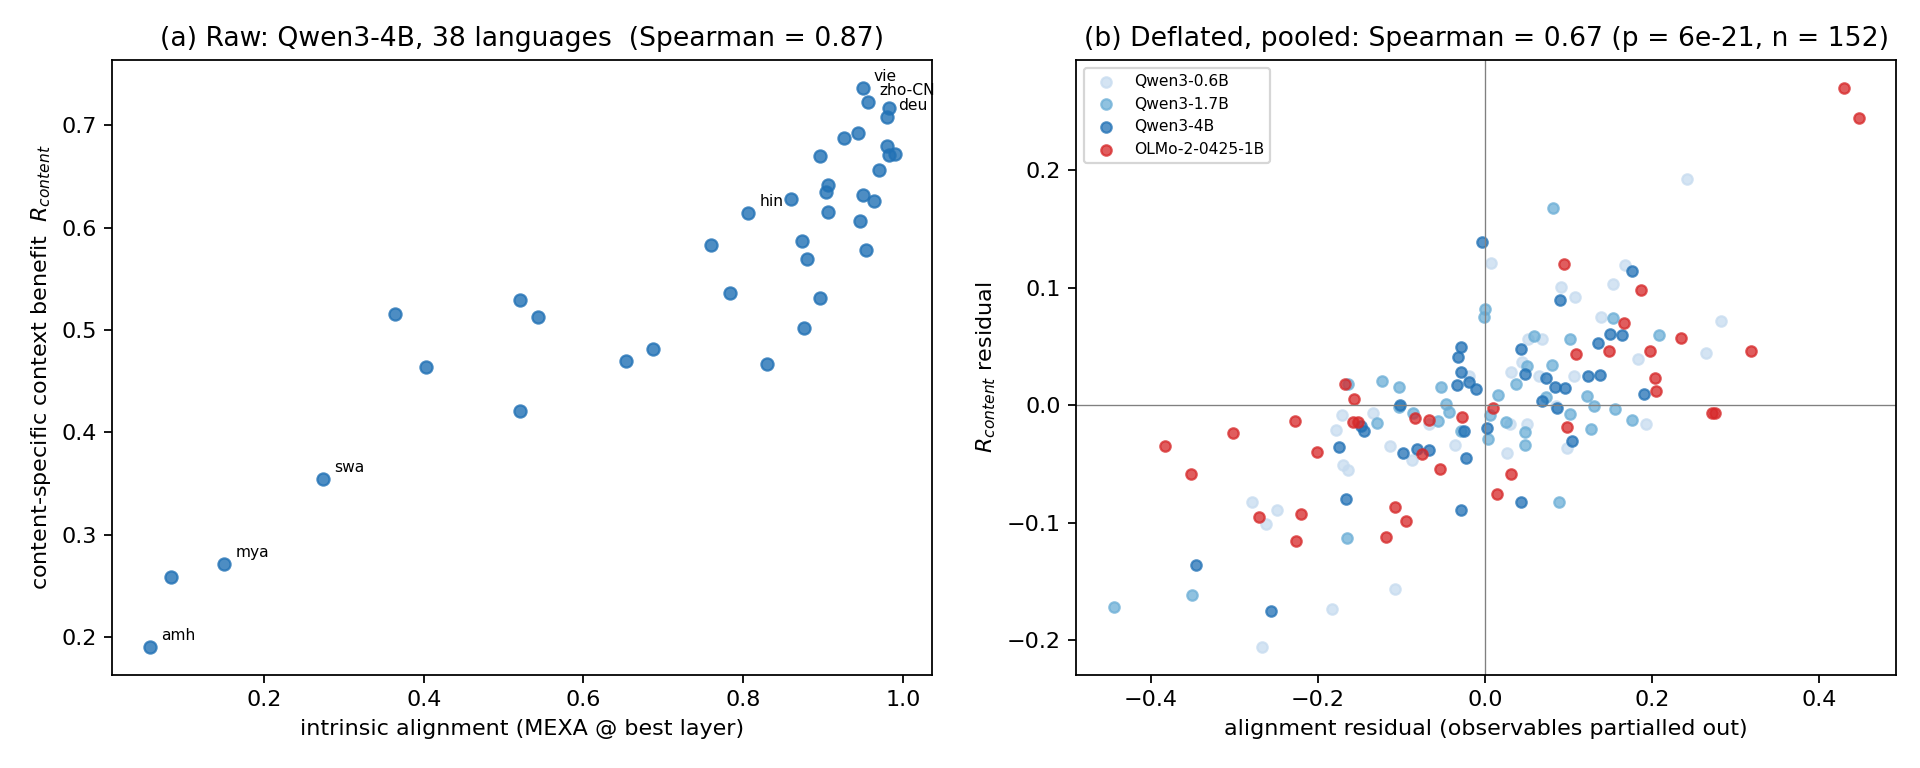
\includegraphics[width=\textwidth]{figs/fig10_b2scatter.png}
  \caption{The predicted-vs-realized plot. (a) Raw: per-language alignment
  vs.\ content-specific context benefit, Qwen3-4B. (b) The same relationship
  after partialling observables out of both axes, pooled over four models:
  what survives ($\rho = 0.67$) is the metric's incremental predictive power.}
  \label{fig:b2scatter}
\end{figure}

\begin{figure}[H]
  \centering
  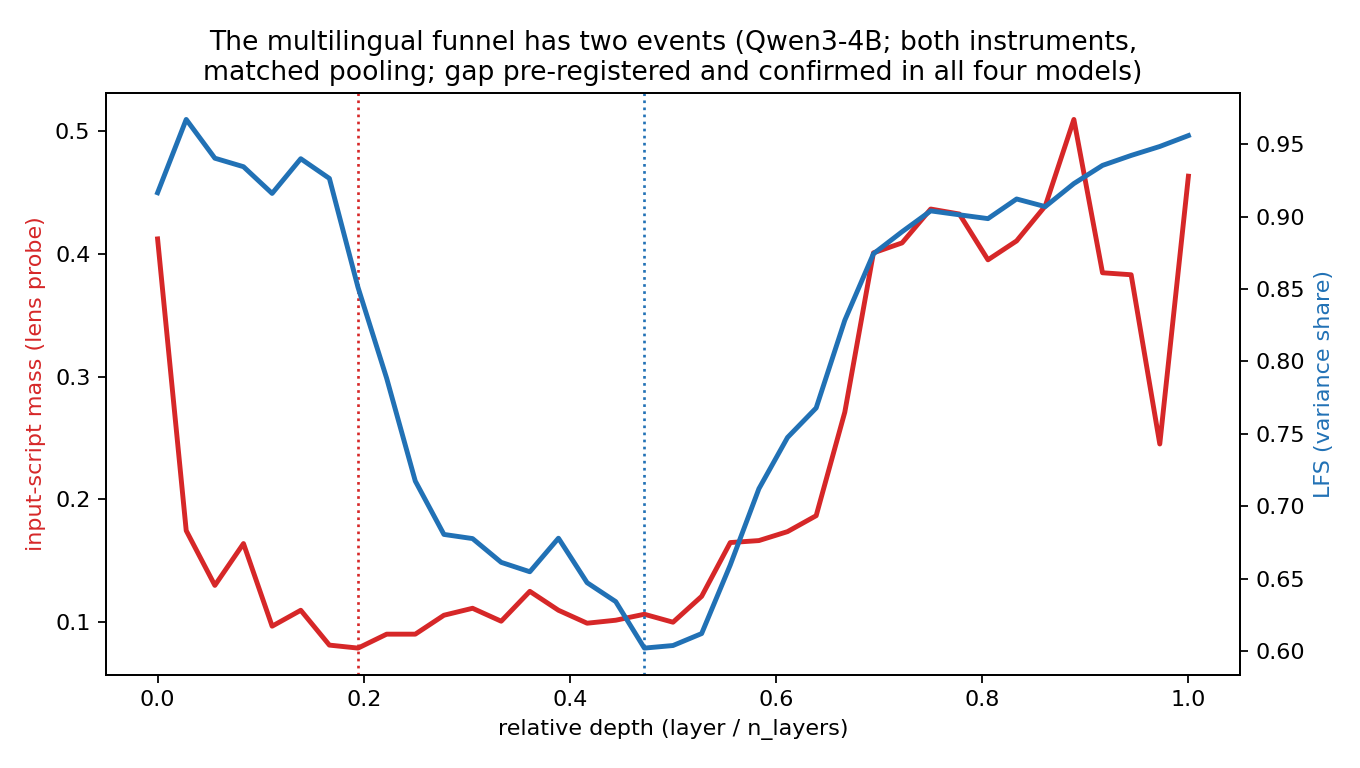
\includegraphics[width=0.8\textwidth]{figs/fig12_twoevents.png}
  \caption{The two-event depth profile, both instruments on one depth axis
  (Qwen3-4B, matched pooling): the lens sees surface script abandoned early;
  LFS sees concept variance converge mid-network.}
  \label{fig:twoevents}
\end{figure}

%==============================================================================
\section{Held-Out Prospective Test: Four of Four, Blind}
%==============================================================================
\label{sec:walkforward}
The metric suite was designed on the 10-model development grid, so the
frozen, pre-registered prospective test (\texttt{WALKFORWARD\_PROTOCOL.md}:
every degree of freedom fixed in advance, including the layer-selection rule
and the benchmark-capable criterion) is the test that separates ``works on our
grid'' from ``works.'' Two never-before-touched families were run:
SmolLM2-1.7B and Falcon3-7B-Base.

\begin{table}[H]
\centering
\small
\caption{Prospective-test scorecard (all predictions frozen before any run).}
\begin{tabular}{p{6.1cm}p{6.6cm}l}
\toprule
Prediction & Outcome & Result \\
\midrule
P1: depth profiles match recipe class & SmolLM2 (EN-centric) dip $0.068$
(predicted shallow, $\leq 0.15$); Falcon3 dip $0.140$ (predicted
intermediate); both dip and recover & PASS \\
P2: attribution criterion holds with 12 models & $\beta_{\mathrm{tokens}} =
+0.272$, $p = 4\times10^{-7}$ & PASS \\
P3: no validity collapse on unseen families & held-out AaR
residual correlation $0.339$, \emph{above} the development-grid CI
$[0.13, 0.30]$ & PASS \\
P4: benchmark-capable subgroup $\Delta$ reproduces (retraction pre-committed
if $\leq 0$) & criterion applied blind: SmolLM2 self-excluded
($0.283 < 0.30$); on Falcon3, $\Delta(\mathrm{AaR}-\mathrm{MEXA}) = +0.136$,
CI $[+0.030, +0.259]$ & PASS \\
\bottomrule
\end{tabular}
\label{tab:walkforward}
\end{table}

Two consequences. First, the design-circularity objection is substantially
narrowed: the
suite classified two unseen families correctly from their training recipes,
under blind scoring. Second, prediction P4 concerned a difference between the tail measure and MEXA on the benchmark-capable subgroup; it passed on the single held-out model that qualified. It is recorded because it was preregistered, and it is not used anywhere in this report as a claim about one measure over another (Appendix~\ref{app:compar}).

\subsection*{A second-generation holdout: Salamandra, pre-registered}
After the prospective test, a modern deliberately-balanced multilingual family
(Salamandra 2B/7B, BSC; $\sim$35 European languages) was run under four
predictions frozen before its first forward pass. Scored: \textbf{P-S1
pass} (interior minimum with endpoint recovery, dip depth $0.288$ at 2B; \emph{deeper than
Qwen3-1.7B}); \textbf{P-S3 pass} (EuroLLM-like European-tier pattern:
EU-8 MEXA $0.94$ vs low-tier $0.03$); \textbf{P-S4 split} (intra-European
donors beat English at 2B, 56\%/44\%, led by Spanish; a training-mix
pattern; but English retakes 56\% of European targets at 7B);
\textbf{P-S2 fail} (the dip \emph{shallows} with scale, $0.288 \to 0.216$,
while alignment improves everywhere: low-tier MEXA $4\times$, EU-8
$0.985$). Two consequences. First, Salamandra resolves the ambiguity BLOOM
left open: deliberate multilingual coverage can coexist with deep concept
convergence, so BLOOM's flat profile reflects its particular recipe and
era rather than coverage-first training as such. Second,
P-S2 is the second observed divergence between the variance-share dip and
retrieval alignment across scale (after the Qwen3-1.7B anomaly): dip depth
is \textbf{not a monotone scaling proxy}, and the two instruments
measure different quantities; the division-of-labor claim, now with
cross-family evidence.

\subsection*{Three added families, pre-registered: granite, Yi, Llama}
\label{sec:newfam}
To widen the benchmark-capable base beyond four families, three new families were
added under frozen predictions (prereg addendum A3, dated before each run):
IBM granite-3.1-8b (the fallback family pre-named in the prospective test
protocol), Yi-1.5-9B, and Llama-3.1-8B. Benchmark capability: \textbf{all three
pass} (0-shot Belebele aggregates $0.337 / 0.453 / 0.471$; predictions
P-A3.1/A3.5 confirmed). Depth profiles: granite dips to depth $0.291$
(in-band); \textbf{Yi falsified its class prediction} (depth $0.140$,
Falcon-like, despite a zh/en-heavy recipe predicted to pattern with Qwen);
and \textbf{Llama-3.1-8B posts one of the two deepest shared spaces in the 17-model grid} (audited depth $0.335$, first-layer value minus minimum, against Qwen3-8B's $0.336$; an earlier draft quoted $0.374$ under a different depth definition); a nominally English-centric
generalist out-converging every deliberately-multilingual model, the
sharpest instance yet of recipe-and-token-scale over design intent. Llama
also provides an unplanned blind replication of the hub finding: the latent
factor beats English for \textbf{124/127 languages}, the same count as most development-grid models (the count ranges from 113 to 124 across the 17 models, with BLOOM lowest), with English best donor for only 25\% of targets. Meta-lesson, disclosed: across Salamandra, Yi, and Llama, our
\emph{a-priori recipe-class guesses} for unseen families ran roughly 50/50
while the instrument itself read every model cleanly on first contact; the strongest argument for measuring over guessing.

\subsection*{Aim-2 feasibility run: the measure moves; the na\"ive objective
is falsified}
Pre-registered with a $\lambda{=}0$ domain-adaptation control: Qwen3-0.6B
fine-tuned for 400 steps with $\mathcal{L} = \mathcal{L}_{\mathrm{LM}} +
\lambda \cdot \mathrm{LFS}_{\mathrm{batch}}$ on training sentences disjoint
from all evaluation data. Results: the LFS dip \textbf{nearly doubles}
($0.206 \to 0.389$; P-A2.1 pass; \emph{the quantity is directly
optimizable}), and
low-tier Belebele improves versus base ($0.257 \to 0.294$; P-A2.4 weak
pass); but alignment transfer \emph{trails} the control (P-A2.2 fail) and
aggregate Belebele drops 2.9 points versus the control's 1.7 (P-A2.3 fail).
Per the pre-committed decision rule: \textbf{LFS-as-objective is falsified
in this na\"ive form}; ratio minimization finds a shortcut (consistent
with partial representation collapse) that deepens the dip without producing
useful convergence. The constructive consequence for Aim~2: the training
objective must be \emph{collapse-resistant}; preserve concept variance
explicitly, or use a contrastive formulation anchored by the LM loss; and the metric suite is the instrument that catches the shortcut.
To be explicit about what this result does and does not say: \textbf{it
falsifies a loss function, not the metric}; measure and target are
different jobs (Goodhart's law, \citealp{goodhart1975,strathern1997}; cf.\ BLEU, which is a serviceable metric and
a degenerate training objective), and it was precisely the suite's
cross-checks that exposed the gamed number. That measure is retained, and
\S\ref{sec:aim2} tests it properly: a six-condition study at three seeds, with
downstream evaluation on held-out sentences and held-out languages, which
supersedes this feasibility result and reaches a sharper conclusion. Combined pre-registration tally
across all validation rounds and holdout additions: \textbf{31 predictions,
21 passed}, every failure reported and informative; the geometry round's
frozen prediction matrix is scored cell-by-cell in \S\ref{sec:boundary}.

%==============================================================================
\section{The Construct Boundary, Measured: Misalignment Decomposition and
Synthetic Test Suite}
%==============================================================================
\label{sec:boundary}
LFS measures the \emph{additive} language share (\S\ref{sec:quant}); rotations,
warps, and concept$\times$language interactions fall into its residual. Round
2 measured that boundary directly, under a pre-registered protocol
(\texttt{prereg/PREREG\_BATTERY.md}, frozen before execution; one dated
addendum, A1, frozen before its patch run).

\subsection{Instruments}
Saved-embedding dumps (parity vs.\ the original grid: worst
$\Delta\mathrm{LFS} = 6\times10^{-7}$, on grid hardware) feed two new
instruments. (1)~A \textbf{misalignment decomposition}: each language is mapped into
a generalized-Procrustes consensus by a nested sequence of maps, offset (M1),
isotropic scale (M2), rotation (M3), general linear (M4), nonlinear kernel
(M5), and each map's share is its \emph{held-out} error reduction,
cross-fitted over 20 stratified splits, with per-language permutation nulls;
negative held-out shares are reported as overfit flags, not clipped. (2)~A
\textbf{synthetic falsification test suite}: ten injection families (offset,
scale, global rotation, per-language rotation, shear, low-rank interaction,
monotone warp, collapse, pairing permutation, identity) applied to the
pre-normalization embeddings at calibrated magnitudes, scored against a
prediction matrix frozen in advance.

\subsection{Calibration}
The instruments read known answers back exactly: injected rotations of
$\theta \in \{0.1, 0.2, 0.4, 0.8\}$ rad are recovered at $0.100/0.200/0.400/
0.800$ in all three prototype models; injected scales are recovered with mean
absolute error $\le 10^{-4}$; identity injections define tight noise floors
($\Delta\mathrm{LFS} \le 0.007$).

\subsection{The decomposition: real misalignment is overwhelmingly additive}
\begin{table}[H]
\centering
\small
\caption{Misalignment decomposition at each model's LFS-dip layer (mean held-out
share across 128 languages; selected rank in parentheses). M5 negative =
kernel-map overfit at $n{=}300$, reported per protocol.}
\begin{tabular}{lrrrrr}
\toprule
 & Offset & Scale & Rotation & Linear & Nonlinear \\
\midrule
Qwen3-1.7B (r=16) & 42.1\% & 23.4\% & 0.06\% & 1.0\% & $-33\%$ \\
OLMo-2-1B (r=16) & 87.6\% & 9.8\% & $-0.1\%$ & 0.4\% & 0.2\% \\
BLOOM-1.7B (r=64) & 59.7\% & 16.5\% & 0.2\% & 3.9\% & $-12\%$ \\
\bottomrule
\end{tabular}
\label{tab:budget}
\end{table}
Offset$+$scale, the structure LFS's decomposition captures, accounts for 65--98\% of held-out cross-language misalignment in these three models and for 63--97\% across all 14 models of the 1,500-sentence study at the common rank 64 (Figure~\ref{fig:budgetcomp}); \textbf{rotation is 0.06--0.2\%} here and never exceeds 0.7\% in the 14-model study.

\begin{figure}[H]
  \centering
  
\includegraphics[width=0.92\textwidth]{figs/fig15_budget_composition.png}
  \caption{Misalignment decomposition composition per model at the dip layer
  (1,500-sentence data, $n = 1500$, common rank $r = 64$ for comparability).
  Additive offset and isotropic scale dominate every model; the rotation
  share, annotated at right, never exceeds $0.7\%$. The gap to 1 is
  idiosyncratic sentence-level variation that no map in the sequence explains;
  negative nonlinear shares are held-out overfitting of the kernel map and are
  annotated rather than drawn.}
  \label{fig:budgetcomp}
\end{figure}

At the 1,500-sentence scale the picture is unchanged and the earlier rank instability
resolves. Across the thirteen selected-rank primaries completed at
$n = 1500$, the one-standard-error rule chooses rank 64 or 128 for every
model; the rank-16 selections seen at $n = 300$ do not recur. Mean rotation
shares span $-0.2\%$ to $+0.7\%$, and the per-language permutation nulls
confirm the same pattern of statistically detectable but practically
negligible structure: the rotation share exceeds its null for 30 to 128 of
128 languages depending on the model while remaining below one percent of
the budget in every case, and the general linear share exceeds its null
almost universally (116 to 128 of 128 languages) while staying between
$0.4\%$ and $8\%$. One model, OLMo-2-1B, is reported without a
selected-rank primary: its permutation-null computation exceeded a 60-hour
allocation twice and was not rerun. Its fixed-rank and centered-subspace
budgets are complete and appear in Figure~\ref{fig:budgetcomp}, and both
place its rotation share below zero, consistent with the rest of the grid.

At prototype scale ($n = 300$), rotation shares are statistically
detectable (76--123 of 128
languages exceed their permutation nulls) but practically negligible.
BLOOM carries the largest general-linear share (3.9\%, 124/128 above null),
consistent with its embedding-layer alignment pattern
(Figure~\ref{fig:profile} discussion). The pre-registered validity test
asked whether rotation or linear shares predict transfer
residual beyond observables \emph{and} alignment: partial Spearman
$\rho = -0.03$ (CI $[-0.16, +0.11]$, $p = 0.73$) and $-0.02$ ($p = 0.76$),
$n = 207$; the pre-registered null branch: \textbf{the additive construct
boundary is empirically harmless on this grid}. Because the procedure
demonstrably detects rotation when present (rotation map $0.15$ at
$\theta = 0.4$ on Qwen3; $0.11$ on BLOOM), the small rotation share means that
additional orthogonal alignment provides little held-out improvement under this protocol. One asymmetry is disclosed: on OLMo-class
(offset-dominated) geometry the rotation map is structurally insensitive
even to centroid-preserving injected rotations (share $\le 0.003$ at
$\theta = 0.8$ with exact angle recovery; addendum A1's pre-committed
fallback); concept variance lies largely outside the top pooled-variance
subspace there, so absence claims are strongest for Qwen3/BLOOM-class
models. A language-centered subspace variant is queued for the 1,500-sentence study.

\subsection{What the test suite caught}
Three pre-registered unexpected results, all reported next to the confirmations.
\textbf{(a) Basis dependence.} A shared \emph{global} rotation; which
preserves all cross-language geometry; moved Qwen3's MEXA, recomputed after re-standardization in the rotated basis, from $0.670$ to $0.094$ (cosine retrieval itself is rotation-invariant; the change comes from the standardization step) and BLOOM's LFS by $-0.32$ (OLMo: mild). Mechanism: per-dimension
z-scoring suppresses massive-activation dimensions in the native basis;
rotation redistributes that variance and the suppression stops working. The
pipeline is therefore \emph{deliberately} basis-dependent: it measures in
the model's computational (neuron) basis. The whitened variant has since
been executed at the 1,500-sentence scale with a pre-registered prediction; and the
prediction failed informatively (see below). \textbf{(b) LFS responds without
attributing.} Rotation, interaction, permutation, and per-language collapse
all \emph{raise} LFS through its concept denominator; broader sensitivity
than we had claimed, with attribution delegated to the decomposition. Two of our
own frozen directional predictions were wrong on this point and are recorded
as such. \textbf{(c) The collapse-gaming result.} Reproducing the Aim-2
study's gaming mode (shrinkage toward the \emph{global} centroid, cell I8b)
showed \textbf{LFS moving by only -0.04 to +0.05 while MEXA stayed within 0.01 and AaR within 0.02 even at 90\% collapse}; retrieval metrics are order-based and structurally blind to
uniform shrinkage. The only instrument that fires is concept-variance
preservation (CVP), and it fires exactly (measured $(1-m)^2$ to three
decimals in all nine cells). We have not found this collapse-blindness of retrieval-based alignment
metrics reported elsewhere (literature sweep of 5 September 2026,
\texttt{docs/LITERATURE\_NOVELTY\_TABLE\_2026-09-05.md}); its consequence is
adopted as policy: \textbf{CVP is a mandatory check for any Aim-2
training objective} (criterion G4).

\subsection{The whitened-basis check: a failed prediction that localizes
the language component}
The pre-registered 1,500-sentence-scale robustness check recomputed dip-layer LFS
after per-layer ZCA whitening on all 14 models of the 1,500-sentence study, with the frozen
prediction that the cross-model ranking would be preserved (Spearman
$> 0.8$). \textbf{The prediction failed}: Spearman $= 0.45$. The mechanism
is itself a finding: whitening collapses the measured language share for 13
of 14 models (e.g.\ SmolLM2 $0.90 \to 0.38$; Salamandra-7B $0.77 \to 0.19$); \textbf{language identity is concentrated in the high-variance
(massive-activation) directions}, so equalizing the spectrum deflates it,
and models differ in \emph{how} concentrated, which reshuffles the middle
of the ranking (the extremes are stable: Qwen3-8B remains deepest,
OLMo-2-1B/SmolLM2 shallowest). Mistral-7B is a clear outlier; essentially unchanged ($0.707 \to 0.699$), its language structure spread
isotropically rather than concentrated: a genuinely different
representational strategy invisible before this check. Retrieval behaves
oppositely: mean MEXA \emph{improves} under whitening for all 14 models,
consistent with the embedding-alignment literature. Consequence: the
measurement basis is a substantive methodological fork, not a footnote;
native-basis comparisons remain internally valid, fine-grained cross-model
orderings of dip depth are reported with this caveat, and both columns
appear wherever ordering matters.

\subsection{Tail curves at the 1,500-sentence scale: the mean-hides-tail finding
becomes a population statistic}
With per-sentence margins retained at $n = 1500$, the AaR tail curve
AaR@\{1, 5, 10, 20\} is estimable per language (AaR@1 is now 15 sentences,
not 3). Three results. First, \textbf{40--50\% of languages in the
strongest models are mean-positive but tail-negative} (Qwen3-4B: 59/128;
Qwen3-1.7B: 57; Qwen3-8B: 48); what was one Hindi anecdote is now the
most common condition; on Qwen3-8B, \emph{Turkish and Greek} carry healthy means
($+0.13$) over failing worst-percentiles ($-0.26$, $-0.24$). Second, tail
\emph{shape} separates model classes: Qwen3 and OLMo-7B show steep
catastrophic-tail profiles (AaR@20$\to$AaR@1 gradient $\approx 0.10$--$0.12$)
while SmolLM2/OLMo-1B/BLOOM are flatter but uniformly weaker; two risk
profiles a mean cannot distinguish. Third, the tail carries information the
mean does not: within-model Spearman between mean margin and AaR@1 falls to
$0.34$ (OLMo-7B). Figure~\ref{fig:tailcurves} shows the curves.

\begin{figure}[H]
  \centering
  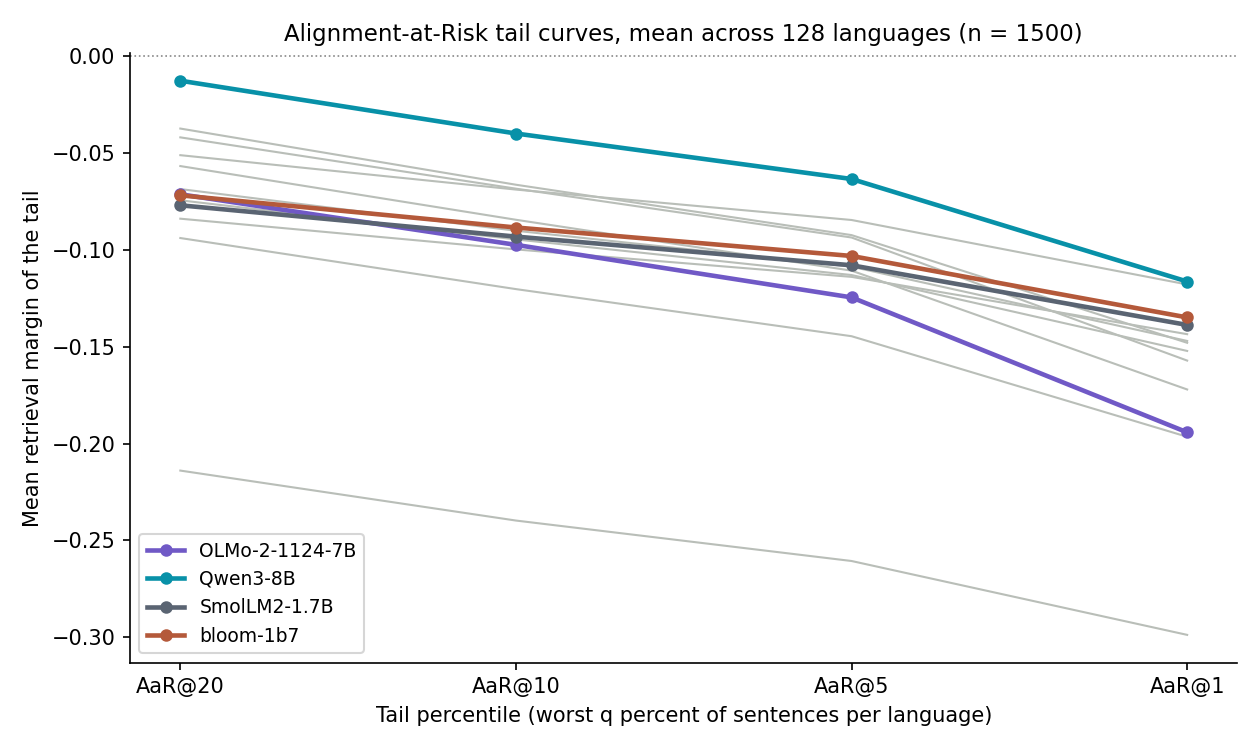
\includegraphics[width=0.82\textwidth]{figs/fig16_tail_curves.png}
  \caption{AaR tail curves (mean across languages) for 13 models of the 1,500-sentence study;
  four representative models highlighted. Steeper descent toward AaR@1
  indicates a catastrophic-tail profile (rare but severe failures);
  a flat low curve indicates broad fragility. Salamandra-2B is omitted for
  axis legibility (its curve sits far below; values in
  \texttt{results/tailcurves/}).}
  \label{fig:tailcurves}
\end{figure}

\subsection{Scope}
Round-2 prototype scope: three models, $n = 300$ sentences/language, dip
layer, translated-news domain. Rank selection was not stable across models
(16/16/64), so the study reports decompositions at both the selected and a
common rank. The $n{=}1500$, 14-model study (including a fresh
balanced-multilingual held-out model, Salamandra) re-runs the decomposition
with per-sentence margins retained; its per-language AaR@\{1, 5, 10, 20\}
tail curves are computed, and the whitened check above is 1,500-sentence-scale.

%==============================================================================
\section{Word-Level Measurement}
\label{sec:wordlevel}
Every measurement above is at the sentence level. Whether the same
decomposition holds when the unit is a single word is a distinct question,
and answering it requires establishing word correspondences that the corpus
does not supply. This section reports what that took and what it found.

\subsection{Alignment reliability, and a gate that failed}
Word correspondences were established between English and each of twenty
languages spanning eleven scripts, using two methodologically independent
aligners: SimAlign over XLM-RoBERTa embeddings and eflomal, a statistical
aligner fitted unsupervised on the parallel text. Their agreement is a
reliability estimate rather than two views of one model.

\textbf{The pre-registered criterion failed.} Agreement above 0.70 F1 was
required on high-resource pairs; two of seven cleared it, mean 0.636.
Agreement tracks typology rather than resource level: Swahili (0.672)
exceeds Russian (0.583) and Arabic (0.553), while the three lowest
non-tokenization cases are agglutinative (Turkish 0.497, Amharic 0.403,
Zulu 0.326), two of them Latin-script. In an agglutinative language a single
word carries what English distributes across several, so a one-to-one
correspondence frequently does not exist to be found. \textbf{The word is a
reliable cross-lingual unit only within a narrow typological band}, and no
aligner can repair that.

A separate and repairable failure affected the four languages written
without whitespace word boundaries. Whitespace tokenization returned whole
clauses as single tokens; Japanese averaged 1.2 tokens per sentence against
English's 20. With standard segmenters (jieba, fugashi, khmer-nltk),
agreement rose from 0.118 to 0.604 for Chinese, 0.096 to 0.502 for Japanese,
and 0.199 to 0.696 for Khmer, with Burmese unchanged as the no-tool control.
For those languages the word is a segmenter's decision rather than an
orthographic fact, and the tool used is recorded per language.

\textbf{Response to the failed criterion.} Rather than discarding languages, the
main link set retains only correspondences that both aligners produce
and that are one-to-one on each side. Reliability is bought with coverage:
mean content-word coverage falls from 0.65 to 0.45, with per-language
retention from 84 percent to 16 percent, and coverage is reported beside
every number.

\subsection{A structural property of word-level multilingual analysis}
The decomposition requires every concept to be present in every language. At
sentence level this is free, because the corpus supplies parallelism. At
word level the concept set is the \emph{intersection} of English positions
aligned in all selected languages, and intersections shrink
multiplicatively. On the full corpus, four languages share 5117 content
concepts, eleven share 1081, and the estimator's pure-noise value rises as
that count falls. Adding languages therefore raises the numerator of
$(L-1)/((L-1)+(N-1))$ while shrinking $N$, and the two effects compound. On
a 300-sentence subset the floor at eleven languages (0.067) overtook the
measured value (0.063) entirely. \textbf{Word-level multilingual analysis
scales badly in the number of languages for reasons of alignment coverage
geometry, not compute}, and this does not arise at sentence level.

\subsection{Results}
With word correspondences established, LFS was computed with concepts as
English word occurrences at two declared operating points. All three gates
pass. Reconstruction, averaging aligned word vectors back to sentences and
comparing against a matched sentence-level computation over the same words,
gives Pearson 1.000 and 0.998. The monolingual null lands within 0.0014 and
0.0001 of the predicted degrees-of-freedom value at grids whose predicted
values differ 28-fold, so the estimator characterization of
\S\ref{sec:nsens} transfers to word level exactly.

\begin{table}[H]
\centering
\small
\caption{Word-level LFS at the dip layer, full corpus, Qwen3-1.7B.}
\begin{tabular}{lrrrr}
\toprule
Operating point & Content concepts & Pure-noise value & Word LFS & Headroom \\
\midrule
11 languages & 1081 & 0.0101 & 0.0686 & 7$\times$ \\
4 languages & 5117 & 0.0008 & 0.0564 & 72$\times$ \\
\bottomrule
\end{tabular}
\end{table}

\textbf{The substantive result is a cross-granularity replication.}
Word-level LFS is minimized at layer 13, which is the layer the
sentence-level analysis independently identifies as this model's dip. This
holds at both operating points and under all three subword-pooling schemes,
six configurations in total. The most language-neutral depth of the network
is the same whether the unit of measurement is a whole sentence or a single
aligned word, which strengthens the sentence-level finding by showing it is
not an artifact of sentence pooling.

\textbf{The directional prediction failed, and its natural interpretation
does not survive a control.} Word-level LFS is lower than the matched
sentence-level value, 0.84$\times$ at eleven languages and 0.51$\times$ at
four, the opposite of what was predicted. The tempting interpretation is that
language identity lives in composition rather than in individual content
words. That interpretation is not supported: on synthetic data with a fixed
per-language offset, independent concept noise, and no linguistic structure
of any kind, averaging items inflates the measured language share on its own
by 3.0$\times$ at four items and 4.6$\times$ at eight. The observed
real-data ratios are smaller than this structureless baseline produces at
comparable counts, so the direction is explained without appeal to language
and no claim is made either way.

The durable consequence is methodological and belongs beside the
evaluation-size result: \textbf{LFS values are not comparable across pooling
granularities}. This is a second dimension along which absolute values must
not be placed side by side, and it sharpens the queued fertility work, since
languages differ systematically in how many subword tokens their sentences
carry.

\subsection{Scope and what remains}
One model. Two corrections stand behind these numbers and are recorded in
the error ledger: an implementation that admitted 35 to 39 percent function
words into a concept set its own protocol restricted to content words, and a
corpus-size choice inherited from the sentence-level convention that left
too few shared concepts to support the broader operating point. A three-way
extension, decomposing by word type, language, and context to expose how
much of a word's representation is context-dependent rather than
identity-fixed, is feasible only at the four-language point (89 types with
at least ten occurrences) and is complicated by the news domain's most
frequent content types being proper nouns, which are transliterated rather
than translated and are therefore cross-lingually invariant for reasons that
have nothing to do with the model.

\section{Pooling and Fertility: What the Depth Profile Depends On}
\label{sec:pooling}
Every representation in this report is a mean over token hidden states.
Mean pooling averages a different number of tokens in each language, because
tokenizer fertility varies, and the word-level analysis established directly
that averaging inflates the measured language share: on synthetic data with a
per-language offset, independent concept noise, and no linguistic structure,
averaging four items raises LFS by $3.0\times$ and eight items by
$4.6\times$. Pooling is therefore not neutral preprocessing, and the
depth profile was re-measured under four schemes on identical sentences and
languages, against a decision rule frozen beforehand
(\texttt{docs/FERTILITY\_ROBUSTNESS\_PLAN.md}).

\textbf{The frozen rule failed for every variant.} It required a cross-model
rank correlation of dip depth above 0.90 and a maximum absolute dip-depth
change below 0.03. Final-token pooling and unit-norm pooling both landed at
exactly 0.900 against a strict inequality, and all variants moved absolute
depth by 0.13 to 0.20, which is comparable to the entire range across
models.

\begin{table}[H]
\centering
\small
\caption{Dip depth under four pooling schemes. Length-matched truncates each
sentence to the per-sentence minimum token count across languages and was
declared a bound rather than a primary comparison in advance, since it
changes which part of the meaning is encoded.}
\begin{tabular}{lrrrr}
\toprule
Model & mean & final-token & unit-norm & length-matched \\
\midrule
Qwen3-0.6B & 0.206 & 0.175 & 0.158 & 0.372 \\
Qwen3-8B & 0.336 & 0.276 & 0.320 & 0.319 \\
OLMo-2-1B & 0.077 & 0.160 & 0.073 & 0.121 \\
BLOOM-1.7B & 0.039 & 0.053 & 0.046 & 0.238 \\
Salamandra-2B & 0.254 & 0.397 & 0.122 & 0.261 \\
\bottomrule
\end{tabular}
\end{table}

\textbf{Magnitude and ordering come apart, and the ordering is the more
robust.} The strongest evidence is structural rather than numerical.
Final-token pooling takes a single position and has \emph{no length
denominator at all}, so it is immune to the mechanism the fertility concern
proposes; if the cross-model ordering were an artifact of that mechanism,
the scheme lacking the mechanism should not reproduce it. It reproduces it
to within a single adjacent transposition among five models.

\textbf{The within-family control is measured, not argued.} Qwen3-0.6B and
Qwen3-8B share a tokenizer, so their fertility is identical by construction.
The scaling result, that the larger model has the deeper shared space, holds
under three of the four schemes and reverses only under the length-matched
bound. Fertility cannot produce a difference between two models whose
fertility is the same number.

\textbf{Fertility is nonetheless present in the representations.}
Correlating tokenizer fertility with each language's contribution to the
language variance at the dip layer, across 127 languages: OLMo-2-1B
$+0.644$, BLOOM $+0.453$, Qwen3-0.6B $+0.432$, Salamandra $+0.417$, all
$p < 10^{-6}$. Languages whose tokenizer fragments them more contribute more
to the measured language variance in every model. Fertility was already a
covariate in the downstream validity regression; this places it on the
representation side, where the concern actually lives, and it means the
depth profile itself carries a fertility component even though the cross-model
ordering does not reduce to it.

\textbf{An exploratory observation, not pre-registered.} Pooling sensitivity
falls sharply with scale. Qwen3-8B varies by 0.060 in depth across the four
schemes and places its minimum within one layer of the same place each time;
Qwen3-0.6B, which shares its tokenizer exactly, varies by 0.214 and scatters
its minimum across layers 3, 8, 12, and 14. If this holds more broadly,
measurement stability is itself a property that improves with scale, and
pooling caveats bind hardest exactly where the shared space is shallowest.

\textbf{Consequences adopted here.} Absolute dip depth is reported as a
mean-pooled quantity throughout. The identity of the dip layer is
pooling-dependent (hypothesis H3 fails), which qualifies every use of the
LFS-selected layer as the place where other instruments are measured;
\S\ref{sec:hardening}d already reported that the main correlations
survive a fixed-depth alternative to that rule, and that check now carries
more weight. Cross-model comparison is considerably more robust than
absolute value. The within-family scaling result is untouched.

%==============================================================================
\section{Aim 2: The Full Study Against the Proposal's Own Specifications}
\label{sec:aim2}
This section reports every Aim~2 experiment run, mapped onto the proposal's
four sub-aims. Twenty-eight training conditions across three seeds, four distinct
objective families, one premise test, and one weight sweep. The main finding is
a negative result about the metric's own construction, and it is the most
consequential finding in this report.

\subsection{What the proposal asks for, and what was run}
\S3.2 states the premise: \emph{``the key to enhanced multilinguality is to
more closely align the representation spaces of the different languages.''}
Its four sub-aims and our coverage:

\begin{table}[H]
\centering
\small
\caption{Aim 2 sub-aims against work completed.}
\begin{tabular}{p{2.4cm}p{5.4cm}p{6.4cm}}
\toprule
Sub-aim & What it specifies & Status \\
\midrule
3.2.1 Data Methods & Code-switched text at word, phrase or sentence
granularity, created from parallel text &
\textbf{Run.} 6 conditions $\times$ 3 seeds at 400 and 2000 steps, word and phrase
granularity, three switch rates, 25\% replay. Sentence granularity and a
parallel-text baseline not built \\[2pt]
3.2.2 Training Objectives & A loss on the difference between
\emph{word} representations for dictionary-linked words; variant with a
language-identity vector subtracted; segment-level pooling ``in addition'' &
\textbf{Run in both forms.} 7 word-level conditions $\times$ 3 seeds, plus the
earlier 6 segment-level conditions. The language-vector variant tested \\[2pt]
3.2.3 Adversarial & A discriminator predicting language identity from
intermediate representations, its accuracy used as a loss &
\textbf{Premise tested, condition not built.} Per-layer language probes, linear
and MLP, against the LFS curve \\[2pt]
3.2.4 Preference & Reward modelling over responses sampled in different
languages & \textbf{Deferred.} Requires generation, sampling and an
instruction-tuned model; out of scope for a base-model study \\
\bottomrule
\end{tabular}
\end{table}

All training used Qwen3-0.6B-Base, 400 steps unless stated, three seeds, on
sentences 500 to 1900 of NTREX, disjoint from every evaluation number in this
report. Evaluation uses the first 300 sentences and reports separately on
trained and held-out languages.

\subsection{The central result: the ratio divides out the failure}
\label{sec:ratiofail}
\S3.2.2 specifies a loss measuring ``the difference between word
representations for the matched words.'' Implemented literally as a squared
difference, that objective is globally minimized at $h = 0$: shrinking every
representation toward zero drives the term to nothing while collapsing the
representation's scale. At initialization the term ran 615 to 2488 against a
language-modelling loss near 10, so it was down-weighted to balance the two
and the drift was logged rather than engineered away, per
\texttt{prereg/PREREG\_WORDALIGN.md}.

It degenerated exactly as pre-registered. Mean representation norm fell from
451 to \textbf{42}, an 89 percent reduction, and the word term fell from 3517
to 1.7. Shrinkage alone accounts for most of that: squared distances scale
with the square of magnitude, so a $10.6\times$ norm reduction predicts a
$113\times$ loss reduction, and the observed $2000\times$ is that plus a
little genuine alignment.

\textbf{Neither LFS nor MEXA detected it.}

\begin{table}[H]
\centering
\small
\caption{The word-level conditions. The collapsed condition posts among the highest retrieval and
the best tail alignment in the study. Only the raw component separates it.}
\begin{tabular}{llrrrrr}
\toprule
Condition & Objective & LFS & MEXA & AaR@10 & CVP & raw $V_{\mathrm{concept}}$ \\
\midrule
WA-A & frozen                 & 0.4446 & 0.4444 & $-0.0902$ & 1.000 & 13791 \\
WA-B & LM only (control)      & 0.4842 & 0.3948 & $-0.0954$ & 1.007 & 13884 \\
WA-C & \textbf{word MSE (the spec)} & 0.4932 & \textbf{0.4878} & \textbf{$-0.0849$} & \textbf{0.051} & \textbf{699} \\
WA-D & + language vector      & 0.4924 & 0.4893 & $-0.0955$ & 0.052 & 704 \\
WA-E & segment MSE            & 0.4787 & 0.4619 & $-0.0952$ & 0.245 & 3385 \\
WA-F & + concept guard        & 0.4975 & 0.4893 & $-0.0846$ & 0.047 & 651 \\
WA-G & \textbf{cosine (sound)}& 0.4826 & 0.3944 & $-0.1040$ & \textbf{1.000} & 13792 \\
\bottomrule
\end{tabular}
\end{table}

Condition WA-C, whose representation norm shrank by 89 percent and holds 5 percent of the frozen
model's concept variance, records \textbf{among the highest mean-case retrieval and
best tail alignment of any condition in this study}. Against the control it gains
$+0.093$ MEXA and $+0.011$ AaR, both clearing their pre-registered minimum
detectable effects of 0.018 and 0.010. Condition WA-G, which does not collapse,
gains nothing: $-0.0004$ MEXA and $-0.009$ AaR.

Both retrieval-based measures rank the scale-collapsed condition first and the
sound condition last.

\textbf{LFS shares the blind spot.} LFS standardizes by the pooled standard
deviation before decomposing, so it is scale-invariant exactly as retrieval
is. It moves from 0.4446 to 0.4932 under an 89 percent norm shrinkage, drifting
mildly in the correct direction but detecting nothing. The reason is
structural: $V_{\mathrm{lang}} / (V_{\mathrm{lang}} + V_{\mathrm{concept}})$
is unchanged when both terms shrink together. \textbf{The ratio divides out
precisely the quantity that failed.}

\begin{figure}[H]
\centering

\includegraphics[width=\textwidth]{figs/fig17_ratio_hides_scale.png}
\caption{The same decomposition, reported two ways. As a ratio, the collapsed
model (0.493) and the sound model (0.483) are a rounding error apart. As
components, they differ by a factor of twenty. The information was never
missing; the ratio discarded it.}
\end{figure}

\paragraph{The consequence for the metric's definition.} The decomposition is
sound and the summary is not. Reporting
$(V_{\mathrm{lang}}, V_{\mathrm{concept}}, \mathrm{residual}, \lVert h \rVert)$
as a profile, with LFS as one derived convenience number, would have caught
every failure in this study. Reporting the share alone caught none of
them. This is the general problem with ratios: a ratio cannot tell you which term
moved, and here the denominator fell off a cliff.

\subsection{Four objective families, and what each did}
\begin{figure}[H]
\centering
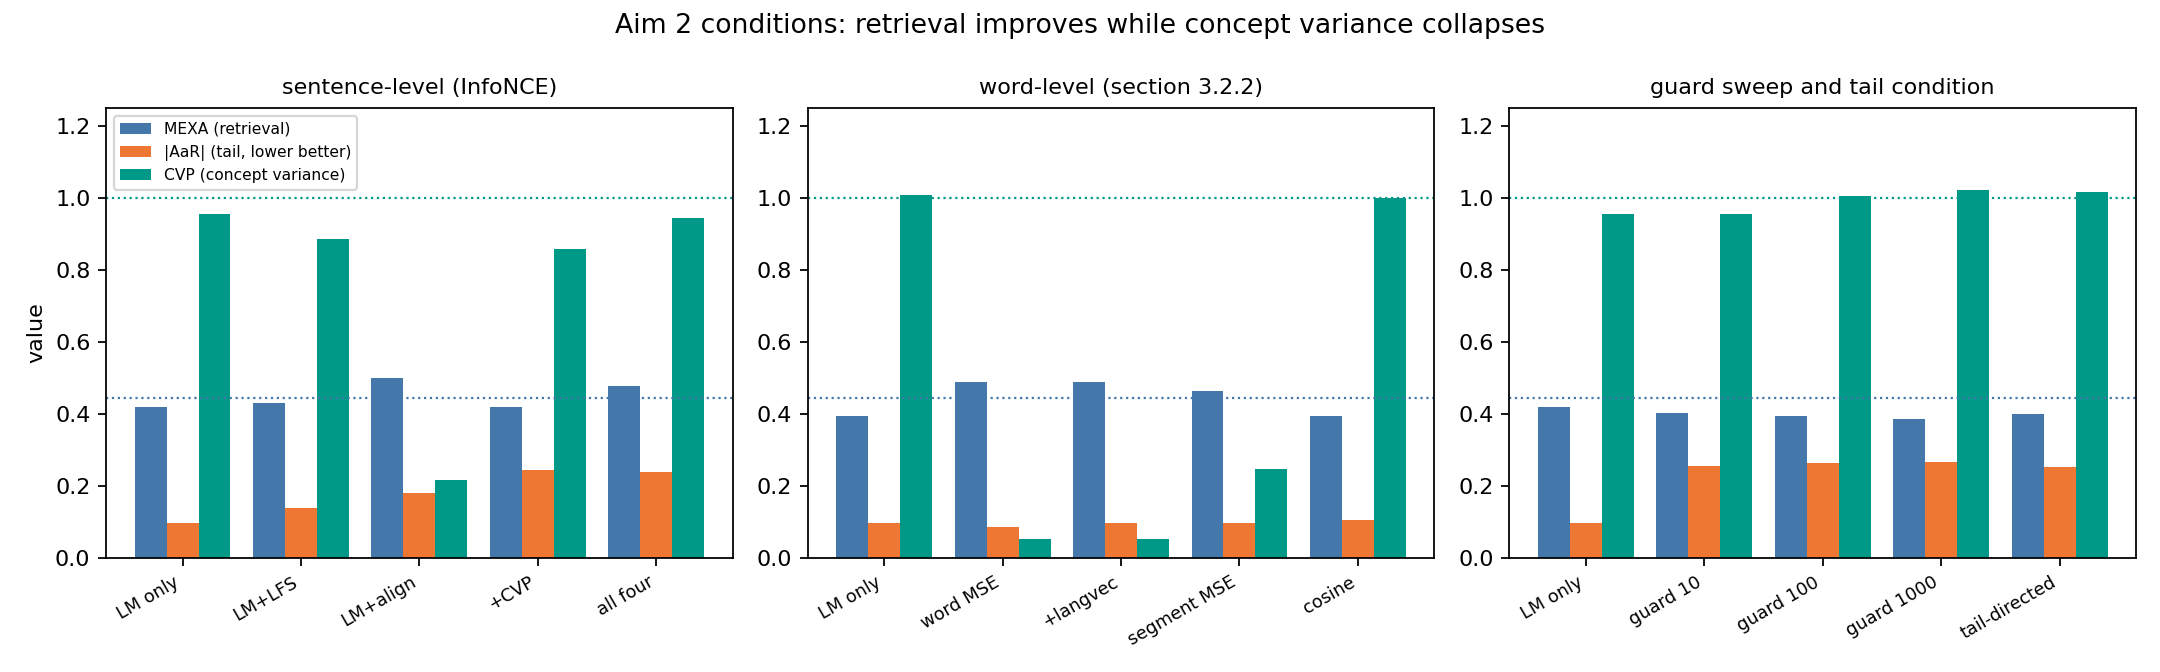
\includegraphics[width=\textwidth]{figs/fig18_aim2_arms.png}
\caption{Every Aim 2 condition on the three instruments. Dotted lines mark the
frozen model's retrieval and unit concept variance. Across all three
families, retrieval rises or holds while concept variance falls.}
\end{figure}

\textbf{Sentence-level contrastive (InfoNCE).} Six conditions. Every condition failed the
seven criteria frozen before running. Across eighteen condition-seed points LFS and
tail alignment moved together at Pearson $+0.924$: every objective that drove
LFS down drove AaR down with it, the opposite of the association observed
across pretrained models. MEXA and AaR decoupled entirely, rank correlation
$-0.067$.

A correction to an earlier measure of these conditions. Condition D's concept variance
ratio of 0.216 was described as a collapse of concept structure. It is not.
Condition D's \emph{standardized} concept variance \emph{rose} from 0.354 to 0.621,
a factor of 1.75, while its raw magnitude fell to 0.216. The structure
improved and the scale shrank, which is the same InfoNCE scale-blindness that
produced WA-C: \texttt{info\_nce} normalizes before computing similarity, so
nothing in it constrains magnitude. Condition E, which did \emph{not} shrink (raw
0.857), posted the worst tail alignment of all at $-0.243$, so scale is not
the mechanism of tail damage.

\textbf{Word-level (\S\ref{sec:ratiofail}).} Reported above. Pre-registered
predictions: P1 degeneracy \textbf{confirmed}; P2 retrieval blind
\textbf{confirmed and exceeded}; P3 language-identity vector helps
\textbf{falsified} ($-0.011$ AaR, wrong direction past its MDE); P4 cosine
does not degenerate \textbf{confirmed} (CVP exactly 1.000); P5 word beats
segment \textbf{confirmed} ($+0.026$ MEXA, $+0.010$ AaR).

\textbf{Code-switched data (\S3.2.1).} Six conditions, three seeds, at 400 and 2000
steps, with an identical 25 percent replay mixture in every condition. No
detectable benefit on any downstream measure: all four criteria returned
\emph{not detectable} against their pre-registered minimum effects, with every
point estimate negative. The cost was neither small nor ambiguous.

\begin{figure}[H]
\centering
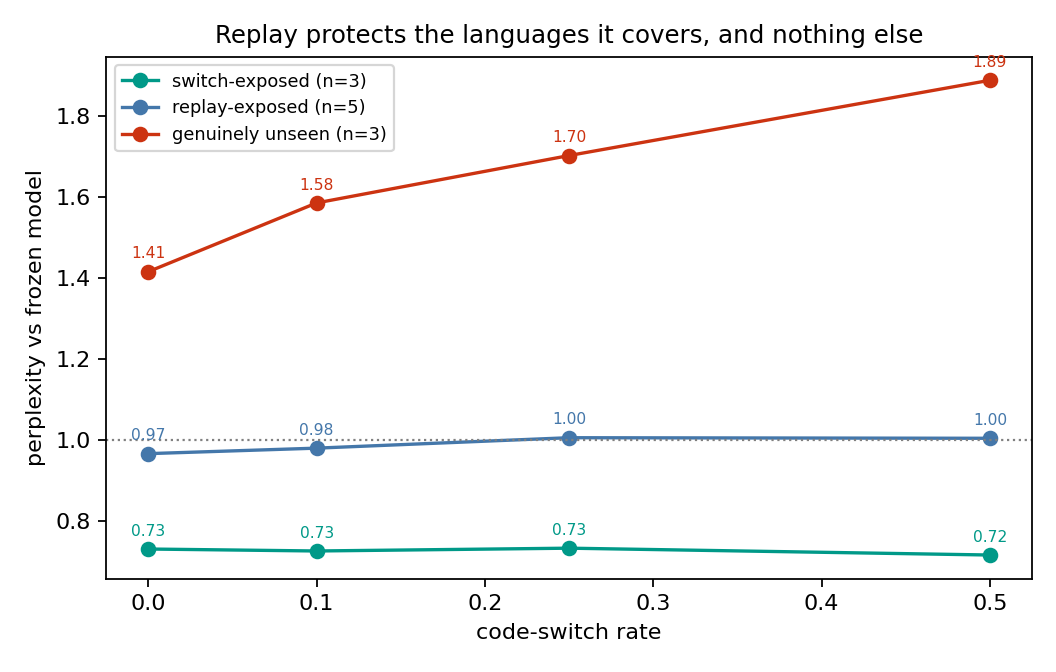
\includegraphics[width=0.72\textwidth]{figs/fig20_codeswitch_cost.png}
\caption{Perplexity against the frozen model by language group. Replay
protects the languages it contains and does nothing for the rest: languages
outside the replay set degrade monotonically with switch rate, to $1.89\times$
at a 50 percent rate, while replay-covered languages stay within four
percent.}
\end{figure}

Replay itself was the one clear success. Without it, the sentence-level conditions
degraded held-out languages by 2.10 to 2.31 times \emph{in every condition including
the control}, which made the capability criterion undiscriminating and wasted
roughly a third of that design. With a 25 percent mixture the control sits at
1.415 and the worst condition at 1.887, and the criterion separates the conditions
cleanly for the first time.

\textbf{Guard weight sweep.} The concept-variance hinge was suspected of being
under-weighted. It is not.

\begin{figure}[H]
\centering
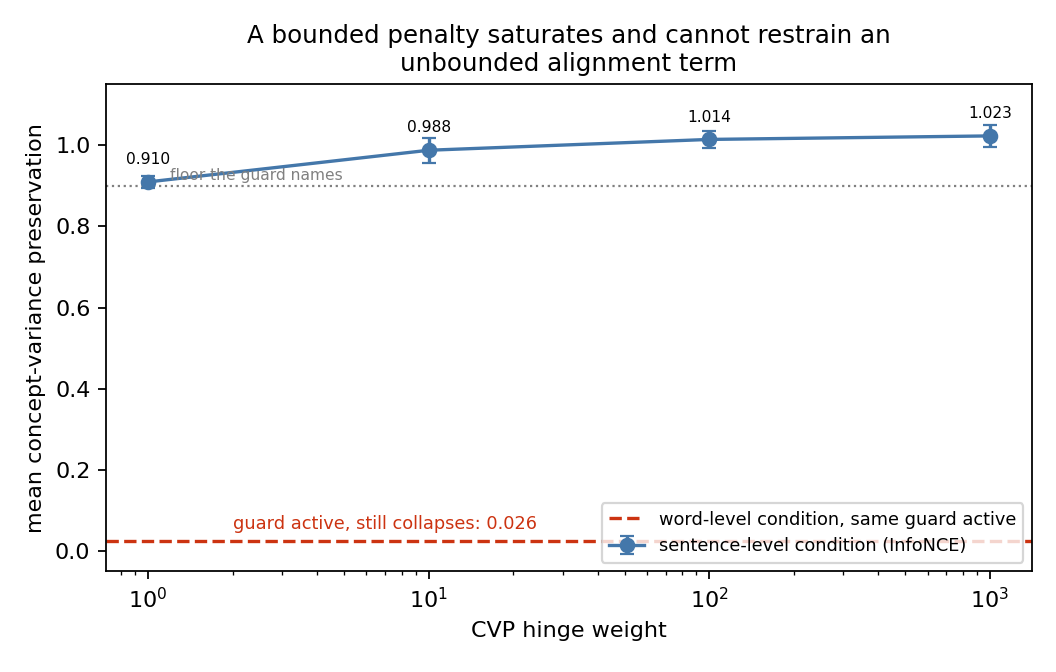
\includegraphics[width=0.72\textwidth]{figs/fig21_guard_sweep.png}
\caption{Raising the hinge weight a thousandfold moves mean concept variance
from 0.910 to 1.023 and then saturates. Against the word-level objective the
same guard, verified active, fails outright.}
\end{figure}

The diagnosis is structural rather than numerical. The hinge is
$(\tau - \mathrm{CVP})^2$ with $\tau = 0.9$, bounded above by 0.81, while the
word-level term starts near 600. \textbf{A bounded penalty saturated at every weight tested, 1 to 1,000, and did not restrain the unbounded term.} With the guard verified active against a frozen
reference, concept variance still fell from 0.051 to 0.002. The remedy is a
hard constraint or a normalized objective, not a larger coefficient.

\subsection{\S3.2.3: does LFS predict what a discriminator can exploit?}
The adversarial method rests on a premise worth testing before it is built. A
discriminator can only succeed to the extent that language-specific variance
exists, and that variance is LFS's numerator. Per-layer language probes were
trained on frozen representations across 24 languages, split by sentence index
so that no concept appears in both train and test.

\begin{figure}[H]
\centering
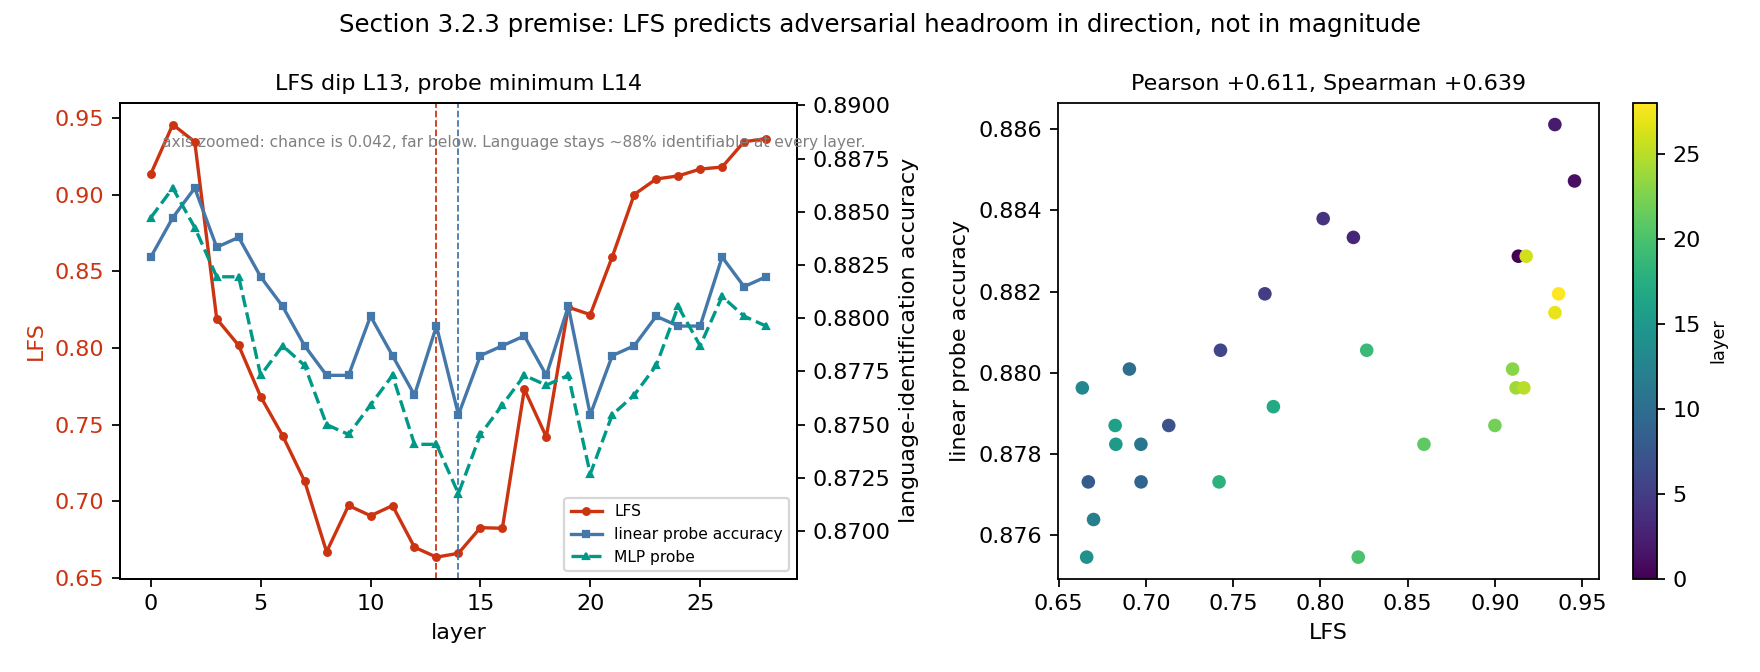
\includegraphics[width=\textwidth]{figs/fig19_adversarial_probe.png}
\caption{LFS against language-identification accuracy across 29 layers. The
curves correlate at Pearson $+0.611$ (MLP $+0.701$) and their minima are
adjacent, at L13 and L14. The tested MLP did not exceed the linear probe.}
\end{figure}

Three findings. \textbf{The premise holds in direction}: LFS and probe
accuracy correlate at $+0.611$ linear and $+0.701$ MLP, and the LFS dip at
L13 sits adjacent to the probe minimum at L14, so LFS locates where
adversarial pressure has the most to remove. \textbf{The additive construct is
adequate}: the MLP gains $-0.002$ over the linear probe on average, so there
is no nonlinear language information for LFS's additive decomposition to
miss. This corroborates the misalignment decomposition, which found rotation
accounts for $-0.205$ to $+0.738$ percent of real misalignment across
thirteen models. \textbf{But the magnitude does not transfer}: LFS spans
0.664 to 0.946 while probe accuracy spans 0.875 to 0.886 against a chance
rate of 0.042. Language remains almost perfectly identifiable at every layer,
including the most language-neutral one. Variance share and separability are
different quantities, and a direction carrying one percent of the variance can
still be perfectly classifiable.

\subsection{Scope and what this does not establish}
One model at 0.6B, 400 steps for most conditions, one layer, and six to fourteen
languages depending on the sub-aim. The word-level alignment links are bounded
by two-aligner agreement of 0.61 to 0.75, so a null on those conditions may reflect
link noise. The loss weighting in the word-level conditions is our choice and not
the proposal's; no sweep over it was run, and a different balance could change
every ordering. \S3.2.1 lacks the parallel-text baseline the proposal treats
as the established comparison, so the code-switch null is measured against
monolingual text rather than against parallel data. No claim is made that
alignment objectives are harmful in general.


\section{What Pre-registration and Checking Caught}
%==============================================================================
\label{sec:discipline}
What transferred was not only formulas but checking habits. Four cases:
\begin{enumerate}
  \item \textbf{Correcting our own main result.} The hub test initially showed
  latent-over-English $+1.04\,R^2$, 26/26 languages. The habit ``too good; find the confound'' revealed a smoothness artifact (a 24-language mean is an
  easier ridge target); the corrected effect is $+0.08$, 113 to 124 of 127 by model. We put the
  corrected number on record before anyone else could find the inflated one.
  \item \textbf{The chance-floor bug.} The first mean-to-spread ratio used raw
  means and crowned BLOOM-1.7B; uniformly at chance in every language,
  hence tiny variance. The ratio must use accuracy above the 4-choice chance floor; with that floor, the ranking inverts to the sensible one.
  \item \textbf{Silent protocol truncation.} The 5-shot evaluation was
  quietly a \emph{different test per model} (context windows 2k--32k);
  detected because a completed run scored below chance on English; the evaluation analog of test-set leakage.
  \item \textbf{Precision as a scientific variable.} fp16 mean-pooling
  overflows on massive activations; BLOOM (bf16-trained) produces
  plausible-looking garbage under fp16 inference. All pooling is fp32;
  BLOOM runs fp32/bf16 only.
\end{enumerate}

%==============================================================================
\section{Limitations}
%==============================================================================
\begin{itemize}
  \item \textbf{Proxy token counts and the sample ledger.} CulturaX sizes
  proxy each model's actual (undisclosed) training mix; exact counts exist
  only for OLMo-2 and BLOOM (robustness subset). Full accounting: $10 \times
  122 = 1{,}220$ potential rows, all with Belebele scores; 410 lack a CulturaX
  token count and 340 lack fertility (overlapping) $\Rightarrow$ 730 fitted;
  correlations use the 690 fitted rows with intrinsic-metric coverage
  (NTREX text availability). With the CC-100 backstop (bytes calibrated to
  the CulturaX token scale on 86 overlap languages, $r{=}0.86$; imputed rows
  flagged), the fit recovers 780 rows and \textbf{100\% of curated
  low-resource rows} (previously 75\%); results strengthen slightly rather
  than weaken ($\beta_{\mathrm{tokens}} = +0.271$, residual correlations
  0.22/0.24). The remaining 28 languages are absent from \emph{both} public
  web corpora; under-resourced beyond the reach of current census data, a
  finding in itself; GlotLID-based counts are the eventual remedy.
  \item \textbf{Mediation.} Residual correlation measures incremental value
  beyond observables; because data size partly \emph{causes} alignment, this
  is a conservative lower bound on metric validity.
  \item \textbf{Additive construct boundary.} The LFS decomposition captures
  language identity as an \emph{additive} main effect; language-specific
  rotations, scalings, and concept$\times$language interactions land in the
  residual and are invisible to the share, so a model could in principle
  score low LFS while still representing concepts differently across
  languages. Now measured (\S\ref{sec:boundary}): rotation is 0.06--0.2\%
  of held-out misalignment and does not predict performance beyond
  observables; the boundary is empirically harmless on this grid, with
  instrument power demonstrated by calibrated injections.
  \item \textbf{Translationese, on both sides of the loop.} NTREX is
  translated from English news; the directional argument that this favors
  English as donor and therefore \emph{understates} the latent-interlingua
  advantage is \textbf{an assumption, not a result}; and
  Belebele is likewise FLORES-derived and English-sourced, so the
  \emph{entire} validation loop currently lives in the translated-news
  domain. The FLORES-200 replication (\S\ref{sec:replication}) now covers the
  corpus side; natively-sourced targets (e.g., TyDiQA-style) remain the
  planned remedy for the benchmark side.
  \item \textbf{Coverage.} Sentence-level primary measurement with a
  word-level check; Qwen3 is the only four-size family in the primary set
  (the expansion set adds Qwen2.5 at four sizes and XGLM at three); no
  model above 13B in either set.
  \item \textbf{Observational validity does not transfer under
  intervention} (\S\ref{sec:aim2}). Every validity number in this report is
  measured across pretrained models that differ in many ways at once. A
  six-condition study at three seeds directly intervened on LFS and found the
  association reverses: driving LFS down drove tail alignment down in all
  eighteen condition-seed points, Pearson $+0.924$. This bounds the use of the
  metric rather than its measurement: \textbf{LFS is a measurement and is not
  a training target}, and none of the confounder-adjusted correlations in this report
  should be read as licensing an intervention.
  \item \textbf{Two frozen gates were mis-specified} (D4, D6), both by
  reasoning about an effect's intended direction without asking what the
  quantity does under the null, and one criterion returned verdicts with no
  power to support them (D7). All are recorded in the discrepancy ledger with
  their replacements proposed and applied prospectively only.
\end{itemize}

%==============================================================================
\section{Next Steps}
%==============================================================================
\label{sec:next}
(1)~\textbf{[Completed; \S\ref{sec:walkforward}]} Prospective test on unseen
families under the frozen protocol: 4/4 blind passes; the benchmark-capable
$\Delta$ reproduced.
(2)~\textbf{[Completed; see Limitations]} CC-100 token backstop: 780
fitted rows, 100\% curated low-tier coverage, results strengthened;
GlotLID counts remain the eventual remedy for the 28 languages absent from
both corpora.
(3)~\textbf{[Completed 5 September 2026; \S\ref{sec:replication}]}
FLORES-200 replication of the 17-model profile (17 of 17 recover; dip-depth
Spearman 0.917 with NTREX), sentence-bootstrap intervals on dip depth, and
six base-versus-instruct pairs. Still open: the 0-shot vs.\ 5-shot agreement
table and a TyDiQA-style natively-sourced extrinsic target (the answer to
the translationese loop).
(3b)~Two named robustness insurances: the \textbf{exact-count subset}; re-run the confounder adjustment using true per-language training counts for the
open-data models (ROOTS for BLOOM, Dolma for OLMo-2); proxy measurement
error biases the tokens coefficient toward zero, so residual confounding in
the residual range cuts \emph{both} ways until this runs; and a
\textbf{fertility-controlled LFS} variant (mean-pooling injects
length/fertility differences into the language component; one sbatch). (4)~\textbf{[Completed; \S\ref{sec:aim2}]} Aim~2 study: six conditions at three
seeds with downstream evaluation. Every condition fails its frozen criteria; the
observational association reverses under intervention; MEXA and AaR decouple;
the collapse guard is necessary and not sufficient. Four follow-ups, in
descending value: a \textbf{replay mixture}, without which held-out
forgetting swamps the capability criterion and roughly a third of the design
is wasted; \textbf{re-specified criteria 2 and 5} per D6 and D7, frozen with
power calculations attached; a \textbf{guard-weight sweep}, since the hinge
currently yields a penalty near 0.0025 against an alignment loss of order
3.4; and an condition that \textbf{optimizes AaR directly} to test the untested
direction of the association.
(4b)~\S3.2.1 code-switched training: the corpus is generated from the Aim~1
word alignments, with per-language aligner agreement in its manifest, and has
not yet been used as training data. It is the cheapest untested sub-aim.
(5)~\textbf{[In progress]} ICLR 2027 submission
(\texttt{paper/iclr2027/main.tex}; abstract registration 18 September 2026,
paper 25 September 2026). The related-work sweep is done
(\texttt{docs/LITERATURE\_NOVELTY\_TABLE\_2026-09-05.md}); the paper makes
no first-of-its-kind claim.
(6)~\textbf{[Completed; \S\ref{sec:boundary}]} Construct-boundary
test suite and misalignment decomposition at $n{=}300$: calibration exact, rotation
0.06--0.2\% of misalignment, teeth null (boundary empirically harmless),
CVP validated as the collapse check.
(7)~\textbf{[Completed, \S\ref{sec:boundary}]} The 1,500-sentence study: the $n{=}1{,}500$ re-embed over 14 models
(including a balanced-multilingual held-out model, Salamandra) retaining
per-sentence margins and selected-layer embeddings: budgets at dual ranks
with a language-centered-subspace variant, the AaR tail curve
AaR@\{1, 5, 10, 20\}, the whitened-pipeline robustness variant, and the
test suite at the larger $n$ (which halved, but did not eliminate, the
kernel-map overfit; the pre-registered prediction that it would vanish is
scored as failed for two of three models in \S\ref{sec:boundary}).

%==============================================================================
\appendix
\section{Record of Comparative Analyses (Retired Framing)}
%==============================================================================
\label{app:compar}
Earlier drafts of this report tested whether the tail measure AaR@10 and the
published measure MEXA differ in confounder-adjusted validity against pooled benchmark
accuracy, and phrased results as ``matches'' or ``edge.'' That framing was
retired on 6 September 2026: the measures answer different questions, and the
proposal asks for a family of metrics, not a winner. The analysis is preserved
here unchanged, as record, so that no result is silently removed.

\paragraph{From \S\ref{sec:hardening}(b), as written in July 2026.}
\textbf{(b) Is the AaR--MEXA difference real? No; and we can prove we
checked.} Two correlations on the same data are dependent; we
cluster-bootstrap languages (2,000 replicates) and form CIs on
$\Delta = \rho_{\mathrm{AaR}} - \rho_{\mathrm{MEXA}}$ under each scheme.
Raw alphas, full grid: $\Delta = +0.033$, 95\%~CI $[+0.001, +0.061]$.
Within-family: $\Delta = -0.013$, CI $[-0.041, +0.014]$; \emph{the sign
flips}. (The within-family scheme demeans across the ``other'' pseudo-family,
a heterogeneous grab-bag of small families; excluding it is a queued
sensitivity line.) AaR's apparent edge lives in the between-family component;
within families the two metrics are statistically indistinguishable. Exploratory
subgroup analyses (e.g., excluding chance-floor models, criterion chosen
post hoc, CI $[+0.001, +0.073]$ barely clearing zero with only 6 model
clusters, where the model-dependence caveat binds hardest) are reported as
exploratory only; the benchmark-capable criterion (aggregate accuracy $\geq 0.30$)
is now \emph{pre-registered} in the prospective-test protocol for blind
confirmation on unseen families. The claim we stand behind:
\textbf{AaR matches MEXA's confounder-adjusted validity while additionally exposing
tail failures that mean-level metrics cannot represent.} Model-level
dependence cannot be cleanly resampled with 10 model clusters;
language-cluster bootstrap is the primary specification; acknowledged,
not solved.

%==============================================================================
\begin{thebibliography}{99}
%==============================================================================
\bibitem[Kargaran et al.(2025)]{kargaran2024mexa}
A.~Kargaran et al. MEXA: Multilingual Evaluation of English-Centric LLMs via
Cross-Lingual Alignment. \emph{Findings of ACL 2025}, arXiv:2410.05873.

\bibitem[Tsvetkov \& Kipnis(2024)]{tsvetkov2024ip}
A.~Tsvetkov, A.~Kipnis. Information Parity: Measuring and Predicting the
Multilingual Capabilities of Language Models. \emph{Findings of EMNLP 2024}.
% verify exact author initials before submission

\bibitem[Dumas et al.(2025)]{dumas2025tongue}
C.~Dumas, C.~Wendler, V.~Veselovsky, G.~Monea, R.~West. Separating Tongue from
Thought: Activation Patching Reveals Language-Agnostic Concept Representations
in Transformers. \emph{ACL 2025}, arXiv:2411.08745.

\bibitem[Shani \& Basirat(2025)]{shani2025shared}
Shani \& Basirat. Language-specific and shared representational spaces in
multilingual language models. 2025.

\bibitem[Wendler et al.(2024)]{wendler2024llamas}
C.~Wendler et al. Do Llamas Work in English? On the Latent Language of
Multilingual Transformers. \emph{ACL 2024}.

\bibitem[Bandarkar et al.(2024)]{bandarkar2024belebele}
L.~Bandarkar et al. The Belebele Benchmark: A Parallel Measure Comprehension
Dataset in 122 Language Variants. \emph{ACL 2024}.

\bibitem[Federmann et al.(2022)]{federmann2022ntrex}
C.~Federmann, T.~Kocmi, Y.~Xin. NTREX-128 -- News Test References for MT
Evaluation of 128 Languages. \emph{SUMEval 2022}.

\bibitem[Nguyen et al.(2023)]{nguyen2023culturax}
T.~Nguyen et al. CulturaX: A Cleaned, Enormous, and Multilingual Dataset for
Large Language Models in 167 Languages. arXiv:2309.09400.

\bibitem[Lin et al.(2019)]{lin2019langrank}
Y.-H.~Lin et al. Choosing Transfer Languages for Cross-Lingual Learning
(LangRank). \emph{ACL 2019}.

\bibitem[Xia et al.(2020)]{xia2020nlperf}
M.~Xia et al. Predicting Performance for Natural Language Processing Tasks
(NLPerf). \emph{ACL 2020}.

\bibitem[Oren et al.(2019)]{oren2019dro}
Y.~Oren, S.~Sagawa, T.~Hashimoto, P.~Liang. Distributionally Robust Language
Modeling. \emph{EMNLP 2019}.

\bibitem[Nitsure et al.(2024)]{nitsure2024risk}
A.~Nitsure, Y.~Mroueh, et al. Risk-aware comparison of foundation models via
tail value-at-risk and stochastic dominance. 2024.
% verify exact title/venue before submission

\bibitem[SHARP(2026)]{sharp2026}
SHARP: Social Harm Analysis via Risk Profiles for Measuring Inequities in
Large Language Models. arXiv:2601.21235.

\bibitem[Zhao et al.(2025)]{zhao2025decompose}
Zhao et al. Decomposing language-specific and language-independent token
representations via SVD, with training-loss applications. 2025.
% exact reference available in the Koehn--Murray proposal bibliography (§2.2)
% — copy it from there before submission

\bibitem[Chang et al.(2022)]{chang2022geometry}
T.~Chang, Z.~Tu, B.~Bergen. The Geometry of Multilingual Language Model
Representations. \emph{EMNLP 2022}.

\bibitem[Timkey \& van Schijndel(2021)]{timkey2021rogue}
W.~Timkey, M.~van Schijndel. All Bark and No Bite: Rogue Dimensions in
Transformer Language Models Obscure Representational Quality. \emph{EMNLP 2021}.

\bibitem[Petrov et al.(2023)]{petrov2023tokenizers}
A.~Petrov et al. Language Model Tokenizers Introduce Unfairness Between
Languages. \emph{NeurIPS 2023}.

\bibitem[Ahia et al.(2023)]{ahia2023costs}
O.~Ahia et al. Do All Languages Cost the Same? Tokenization in the Era of
Commercial Language Models. \emph{EMNLP 2023}.

\bibitem[Koehn \& Murray(2026)]{koehn2026proposal}
P.~Koehn, K.~Murray. Understanding and Improving Multilinguality of Large
Language Models. NSF proposal, Johns Hopkins University.

\bibitem[Bayazit et al.(2026)]{bayazit2026lingua}
D.~Bayazit, B.~AlKhamissi, A.~Bosselut. Lingua Franca or Probing Artifact?
Rethinking Latent Language in Multilingual LLMs. arXiv:2609.00155, 2026.
\bibitem[Sakajo et al.(2026)]{sakajo2026structural}
H.~Sakajo, Y.~Sakai, H.~Kamigaito, T.~Watanabe. Multilinguality of Large
Language Models From a Structural Perspective. arXiv:2606.01800, 2026.
\bibitem[Marinov et al.(2026)]{marinov2026separability}
B.~Marinov, A.~Sharma, C.~Schroeder de Witt, P.~Torr, A.~Calinescu, J.~Yu.
When Language Representations Interact: Separability and Cross-Lingual
Effects in LLMs. arXiv:2606.14347, 2026.
\bibitem[Ravisankar et al.(2025)]{ravisankar2025map}
K.~Ravisankar, H.~Han, S.~Wiegreffe, M.~Carpuat. Can you map it to English?
The Role of Cross-Lingual Alignment in Multilingual Performance of LLMs.
arXiv:2504.09378, 2025.
\bibitem[Liang et al.(2021)]{liang2021locating}
S.~Liang, P.~Dufter, H.~Sch\"utze. Locating Language-Specific Information in
Contextualized Embeddings. arXiv:2109.08040, 2021.
\bibitem[Xie et al.(2022)]{xie2022lowrank}
Z.~Xie, H.~Zhao, T.~Yu, S.~Li. Discovering Low-rank Subspaces for
Language-agnostic Multilingual Representations. \emph{EMNLP 2022}.
\bibitem[Fisher(1925)]{fisher1925}
R.~A.~Fisher. \emph{Statistical Methods for Research Workers}. Oliver and
Boyd, 1925.
\bibitem[Ross(1976)]{ross1976apt}
S.~A.~Ross. The arbitrage theory of capital asset pricing. \emph{Journal of
Economic Theory} 13(3):341--360, 1976.
\bibitem[Fama and French(1993)]{fama1993factors}
E.~F.~Fama, K.~R.~French. Common risk factors in the returns on stocks and
bonds. \emph{Journal of Financial Economics} 33(1):3--56, 1993.
\bibitem[Sharpe(1966)]{sharpe1966}
W.~F.~Sharpe. Mutual fund performance. \emph{Journal of Business}
39(1):119--138, 1966.
\bibitem[Jensen(1968)]{jensen1968}
M.~C.~Jensen. The performance of mutual funds in the period 1945--1964.
\emph{Journal of Finance} 23(2):389--416, 1968.
\bibitem[Artzner et al.(1999)]{artzner1999coherent}
P.~Artzner, F.~Delbaen, J.-M.~Eber, D.~Heath. Coherent measures of risk.
\emph{Mathematical Finance} 9(3):203--228, 1999.
\bibitem[Rockafellar and Uryasev(2000)]{rockafellar2000cvar}
R.~T.~Rockafellar, S.~Uryasev. Optimization of conditional value-at-risk.
\emph{Journal of Risk} 2(3):21--41, 2000.
\bibitem[Bailey and L\'opez de Prado(2014)]{bailey2014deflated}
D.~H.~Bailey, M.~L\'opez de Prado. The deflated Sharpe ratio: correcting for
selection bias, backtest overfitting, and non-normality. \emph{Journal of
Portfolio Management} 40(5):94--107, 2014.
\bibitem[L\'opez de Prado(2018)]{lopezdeprado2018}
M.~L\'opez de Prado. \emph{Advances in Financial Machine Learning}. Wiley,
2018.
\bibitem[Goodhart(1975)]{goodhart1975}
C.~A.~E.~Goodhart. Problems of monetary management: the U.K. experience.
\emph{Papers in Monetary Economics}, Volume 1, Reserve Bank of Australia,
1975.
\bibitem[Strathern(1997)]{strathern1997}
M.~Strathern. `Improving ratings': audit in the British university system.
\emph{European Review} 5(3):305--321, 1997.
\bibitem[Gonen et al.(2020)]{gonen2020greek}
H.~Gonen, S.~Ravfogel, Y.~Elazar, Y.~Goldberg. It's not Greek to mBERT: Inducing Word-Level Translations from Multilingual BERT. \emph{Proceedings of the Third BlackboxNLP Workshop on Analyzing and Interpreting Neural Networks for NLP}, pp.~45--56, 2020.
\bibitem[Zhao et al.(2021)]{zhao2021inducing}
W.~Zhao, S.~Eger, J.~Bjerva, I.~Augenstein. Inducing Language-Agnostic Multilingual Representations. \emph{Proceedings of *SEM 2021: The Tenth Joint Conference on Lexical and Computational Semantics}, pp.~229--240, 2021.
\bibitem[Kojima et al.(2024)]{kojima2024neurons}
T.~Kojima, I.~Okimura, Y.~Iwasawa, H.~Yanaka, Y.~Matsuo. On the Multilingual Ability of Decoder-based Pre-trained Language Models: Finding and Controlling Language-Specific Neurons. \emph{Proceedings of the 2024 Conference of the North American Chapter of the Association for Computational Linguistics: Human Language Technologies (Volume 1: Long Papers)}, pp.~6919--6971, 2024.
\bibitem[Zhao et al.(2025)]{zhao2025disentanglement}
W.~Zhao, J.~Guo, Y.~Deng, T.~Wu, W.~Zhang, Y.~Hu, X.~Sui, Y.~Zhao, W.~Che, B.~Qin, T. S.~Chua, T.~Liu. When Less Language is More: Language-Reasoning Disentanglement Makes LLMs Better Multilingual Reasoners. \emph{Advances in Neural Information Processing Systems (NeurIPS 2025)}, 2025.
\bibitem[Lopo et al.(2025)]{lopo2025surgery}
J. A.~Lopo, M. R. S.~Habibi, T. H.~Wong, M. I.~Ghozali, F.~Koto, G. I.~Winata, P.~Limkonchotiwat, A. F.~Aji, S.~Cahyawijaya. Language Surgery in Multilingual Large Language Models. \emph{Proceedings of the 5th Workshop on Multilingual Representation Learning (MRL 2025)}, pp.~438--467, 2025.
\bibitem[Zhong et al.(2025)]{zhong2025think}
C.~Zhong, Q.~Liu, F.~Cheng, J.~Jiang, Z.~Wan, C.~Chu, Y.~Murawaki, S.~Kurohashi. What Language Do Non-English-Centric Large Language Models Think in? \emph{Findings of the Association for Computational Linguistics: ACL 2025}, pp.~26333--26346, 2025.
\bibitem[Deng et al.(2025)]{deng2025unveiling}
B.~Deng, Y.~Wan, B.~Yang, Y.~Zhang, F.~Feng. Unveiling Language-Specific Features in Large Language Models via Sparse Autoencoders. \emph{Proceedings of the 63rd Annual Meeting of the Association for Computational Linguistics (Volume 1: Long Papers)}, pp.~4563--4608, 2025.
\bibitem[Zeng et al.(2025)]{zeng2025converging}
H.~Zeng, S.~Han, L.~Chen, K.~Yu. Converging to a Lingua Franca: Evolution of Linguistic Regions and Semantics Alignment in Multilingual Large Language Models. \emph{Proceedings of the 31st International Conference on Computational Linguistics (COLING 2025)}, pp.~10602--10617, 2025.
\bibitem[Cheng et al.(2025)]{cheng2025abstraction}
E.~Cheng, D.~Doimo, C.~Kervadec, I.~Macocco, J.~Yu, A.~Laio, M.~Baroni. Emergence of a High-Dimensional Abstraction Phase in Language Transformers. \emph{Proceedings of the Thirteenth International Conference on Learning Representations (ICLR 2025)}, 2025.
\bibitem[Lauscher et al.(2020)]{lauscher2020hero}
A.~Lauscher, V.~Ravishankar, I.~Vuli\'c, G.~Glava\v{s}. From Zero to Hero: On the Limitations of Zero-Shot Language Transfer with Multilingual Transformers. \emph{Proceedings of the 2020 Conference on Empirical Methods in Natural Language Processing (EMNLP)}, pp.~4483--4499, 2020.
\bibitem[Ali et al.(2024)]{ali2024tokenizer}
M.~Ali, M.~Fromm, K.~Thellmann, R.~Rutmann, M.~L\"ubbering, J.~Leveling, K.~Klug, J.~Ebert, N.~Doll, J.~Buschhoff, C.~Jain, A.~Weber, L.~Jurkschat, H.~Abdelwahab, C.~John, P.~Ortiz Suarez, M.~Ostendorff, S.~Weinbach, R.~Sifa, S.~Kesselheim, N.~Flores-Herr. Tokenizer Choice For LLM Training: Negligible or Crucial? \emph{Findings of the Association for Computational Linguistics: NAACL 2024}, pp.~3907--3924, 2024.
\bibitem[Bagheri Nezhad \& Agrawal(2024)]{bagherinezhad2024drives}
S.~Bagheri Nezhad, A.~Agrawal. What Drives Performance in Multilingual Language Models? \emph{Proceedings of the Eleventh Workshop on NLP for Similar Languages, Varieties, and Dialects (VarDial 2024)}, pp.~16--27, 2024.
\bibitem[Wu et al.(2025)]{wu2025bitter}
M.~Wu, W.~Wang, S.~Liu, H.~Yin, X.~Wang, Y.~Zhao, C.~Lyu, L.~Wang, W.~Luo, K.~Zhang. The Bitter Lesson Learned from 2,000+ Multilingual Benchmarks. \emph{arXiv preprint arXiv:2504.15521}, 2025.
\bibitem[Idris et al.(2026)]{idris2026embedding}
T. K.~Idris, P.~Mitra, R.~Eiselen. Can Embedding Similarity Predict Cross-Lingual Transfer? A Systematic Study on African Languages. \emph{arXiv preprint arXiv:2601.03168}, 2026.
\bibitem[Rudman et al.(2022)]{rudman2022isoscore}
W.~Rudman, N.~Gillman, T.~Rayne, C.~Eickhoff. IsoScore: Measuring the Uniformity of Embedding Space Utilization. \emph{Findings of the Association for Computational Linguistics: ACL 2022}, pp.~3325--3339, 2022.
\bibitem[H\"ammerl et al.(2023)]{hammerl2023anisotropy}
K.~H\"ammerl, A.~Fastowski, J.~Libovick\'y, A.~Fraser. Exploring Anisotropy and Outliers in Multilingual Language Models for Cross-Lingual Semantic Sentence Similarity. \emph{Findings of the Association for Computational Linguistics: ACL 2023}, pp.~7023--7037, 2023.
\bibitem[Ding et al.(2021)]{ding2021grounding}
F.~Ding, J. S.~Denain, J.~Steinhardt. Grounding Representation Similarity Through Statistical Testing. \emph{Advances in Neural Information Processing Systems 34 (NeurIPS 2021)}, 2021.
\bibitem[Kriegeskorte \& Diedrichsen(2019)]{kriegeskorte2019onion}
N.~Kriegeskorte, J.~Diedrichsen. Peeling the Onion of Brain Representations. \emph{Annual Review of Neuroscience}, pp.~407--432, 2019.
\bibitem[Chi et al.(2021)]{chi2021infoxlm}
Z.~Chi, L.~Dong, F.~Wei, N.~Yang, S.~Singhal, W.~Wang, X.~Song, X. L.~Mao, H.~Huang, M.~Zhou. InfoXLM: An Information-Theoretic Framework for Cross-Lingual Language Model Pre-Training. \emph{Proceedings of the 2021 Conference of the North American Chapter of the Association for Computational Linguistics: Human Language Technologies}, pp.~3576--3588, 2021.
\bibitem[Bardes et al.(2022)]{bardes2022vicreg}
A.~Bardes, J.~Ponce, Y.~LeCun. VICReg: Variance-Invariance-Covariance Regularization for Self-Supervised Learning. \emph{Proceedings of the Tenth International Conference on Learning Representations (ICLR 2022)}, 2022.
\bibitem[Ji et al.(2024)]{ji2024emma}
S.~Ji, Z.~Li, J.~Paavola, P.~Lin, P.~Chen, D.~O'Brien, H.~Luo, H.~Sch\"utze, J.~Tiedemann, B.~Haddow. EMMA-500: Enhancing Massively Multilingual Adaptation of Large Language Models. \emph{arXiv preprint arXiv:2409.17892}, 2024.
\bibitem[Gao et al.(2023)]{gao2023scaling}
L.~Gao, J.~Schulman, J.~Hilton. Scaling Laws for Reward Model Overoptimization. \emph{Proceedings of the 40th International Conference on Machine Learning (ICML 2023)}, pp.~10835--10866, 2023.
\bibitem[Conneau et al.(2020)]{conneau2020emerging}
A.~Conneau, S.~Wu, H.~Li, L.~Zettlemoyer, V.~Stoyanov. Emerging Cross-lingual Structure in Pretrained Language Models. \emph{Proceedings of the 58th Annual Meeting of the Association for Computational Linguistics}, pp.~6022--6034, 2020.
\bibitem[Tiyajamorn et al.(2021)]{tiyajamorn2021representation}
N.~Tiyajamorn, T.~Kajiwara, Y.~Arase, M.~Onizuka. Language-agnostic Representation from Multilingual Sentence Encoders for Cross-lingual Similarity Estimation. \emph{Proceedings of the 2021 Conference on Empirical Methods in Natural Language Processing}, pp.~7764--7774, 2021.
\bibitem[Huang et al.(2024)]{huang2024erasure}
Z.~Huang, P.~Yu, S.~Ravfogel, J.~Allan. Language Concept Erasure for Language-invariant Dense Retrieval. \emph{Proceedings of the 2024 Conference on Empirical Methods in Natural Language Processing}, pp.~13261--13273, 2024.
\bibitem[Sterz et al.(2025)]{sterz2025recover}
H.~Sterz, F. D.~Schmidt, G.~Glava\v{s}, I.~Vuli\'c. ReCoVeR the Target Language: Language Steering without Sacrificing Task Performance. \emph{Findings of the Association for Computational Linguistics: EMNLP 2025}, pp.~19390--19405, 2025.
\bibitem[Kim et al.(2026)]{kim2026langsae}
D.~Kim, J.~Yoon, C.~Park, H.~Lim. LangSAE Editing: Improving Multilingual Information Retrieval via Post-hoc Language Identity Removal. \emph{arXiv preprint arXiv:2601.04768}, 2026.
\bibitem[Tang et al.(2024)]{tang2024neurons}
T.~Tang, W.~Luo, H.~Huang, D.~Zhang, X.~Wang, X.~Zhao, F.~Wei, J. R.~Wen. Language-Specific Neurons: The Key to Multilingual Capabilities in Large Language Models. \emph{Proceedings of the 62nd Annual Meeting of the Association for Computational Linguistics (Volume 1: Long Papers)}, pp.~5701--5715, 2024.
\bibitem[Harrasse et al.(2025)]{harrasse2025transcoders}
A.~Harrasse, F.~Draye, P. S.~Pandey, Z.~Jin, B.~Sch\"olkopf. Tracing Multilingual Representations in LLMs with Cross-Layer Transcoders. \emph{arXiv preprint arXiv:2511.10840}, 2025.
\bibitem[K\"orner et al.(2026)]{korner2026meanings}
F.~K\"orner, M.~M\"uller-Eberstein, A.~Korhonen, B.~Plank. When Meanings Meet: Investigating the Emergence and Quality of Shared Concept Spaces during Multilingual Language Model Training. \emph{Proceedings of the 19th Conference of the European Chapter of the Association for Computational Linguistics (Volume 1: Long Papers)}, pp.~3149--3169, 2026.
\bibitem[Skean et al.(2025)]{skean2025layer}
O.~Skean, M. R.~Arefin, D.~Zhao, N. N.~Patel, J.~Naghiyev, Y.~LeCun, R.~Shwartz-Ziv. Layer by Layer: Uncovering Hidden Representations in Language Models. \emph{Proceedings of the 42nd International Conference on Machine Learning}, pp.~55854--55875, 2025.
\bibitem[Artetxe et al.(2020)]{artetxe2020artifacts}
M.~Artetxe, G.~Labaka, E.~Agirre. Translation Artifacts in Cross-lingual Transfer Learning. \emph{Proceedings of the 2020 Conference on Empirical Methods in Natural Language Processing (EMNLP)}, pp.~7674--7684, 2020.
\bibitem[Gaschi et al.(2023)]{gaschi2023alignment}
F.~Gaschi, P.~Cerda, P.~Rastin, Y.~Toussaint. Exploring the Relationship between Alignment and Cross-lingual Transfer in Multilingual Transformers. \emph{Findings of the Association for Computational Linguistics: ACL 2023}, pp.~3020--3042, 2023.
\bibitem[Singh et al.(2025)]{singh2025globalmmlu}
S.~Singh, A.~Romanou, C.~Fourrier, D. I.~Adelani, J. G.~Ngui, D.~Vila-Suero, P.~Limkonchotiwat, K.~Marchisio, W. Q.~Leong, Y.~Susanto, R.~Ng, S.~Longpre, S.~Ruder, W. Y.~Ko, A.~Bosselut, A.~Oh, A.~Martins, L.~Choshen, D.~Ippolito, E.~Ferrante, M.~Fadaee, B.~Ermis, S.~Hooker. Global MMLU: Understanding and Addressing Cultural and Linguistic Biases in Multilingual Evaluation. \emph{Proceedings of the 63rd Annual Meeting of the Association for Computational Linguistics (Volume 1: Long Papers)}, pp.~18761--18799, 2025.
\bibitem[Miller(2024)]{miller2024evals}
E.~Miller. Adding Error Bars to Evals: A Statistical Approach to Language Model Evaluations. \emph{arXiv preprint arXiv:2411.00640}, 2024.
\bibitem[Ethayarajh(2019)]{ethayarajh2019contextual}
K.~Ethayarajh. How Contextual are Contextualized Word Representations? Comparing the Geometry of BERT, ELMo, and GPT-2 Embeddings. \emph{Proceedings of the 2019 Conference on Empirical Methods in Natural Language Processing and the 9th International Joint Conference on Natural Language Processing (EMNLP-IJCNLP)}, pp.~55--65, 2019.
\bibitem[Kovaleva et al.(2021)]{kovaleva2021outlier}
O.~Kovaleva, S.~Kulshreshtha, A.~Rogers, A.~Rumshisky. BERT Busters: Outlier Dimensions that Disrupt Transformers. \emph{Findings of the Association for Computational Linguistics: ACL-IJCNLP 2021}, pp.~3392--3405, 2021.
\bibitem[Sun et al.(2024)]{sun2024massive}
M.~Sun, X.~Chen, J. Z.~Kolter, Z.~Liu. Massive Activations in Large Language Models. \emph{First Conference on Language Modeling (COLM)}, 2024.
\bibitem[Hewitt \& Liang(2019)]{hewitt2019control}
J.~Hewitt, P.~Liang. Designing and Interpreting Probes with Control Tasks. \emph{Proceedings of the 2019 Conference on Empirical Methods in Natural Language Processing and the 9th International Joint Conference on Natural Language Processing (EMNLP-IJCNLP)}, pp.~2733--2743, 2019.
\bibitem[Cao et al.(2020)]{cao2020alignment}
S.~Cao, N.~Kitaev, D.~Klein. Multilingual Alignment of Contextual Word Representations. \emph{International Conference on Learning Representations (ICLR)}, 2020.
\bibitem[Wang \& Isola(2020)]{wang2020uniformity}
T.~Wang, P.~Isola. Understanding Contrastive Representation Learning through Alignment and Uniformity on the Hypersphere. \emph{Proceedings of the 37th International Conference on Machine Learning}, pp.~9929--9939, 2020.
\bibitem[Conneau et al.(2020)]{conneau2020unsupervised}
A.~Conneau, K.~Khandelwal, N.~Goyal, V.~Chaudhary, G.~Wenzek, F.~Guzm\'an, E.~Grave, M.~Ott, L.~Zettlemoyer, V.~Stoyanov. Unsupervised Cross-lingual Representation Learning at Scale. \emph{Proceedings of the 58th Annual Meeting of the Association for Computational Linguistics}, pp.~8440--8451, 2020.
\bibitem[Da Silva et al.(2025)]{dasilva2025steering}
P. Q.~Da Silva, H.~Sethuraman, D.~Rajagopal, H.~Hajishirzi, S.~Kumar. Steering off Course: Reliability Challenges in Steering Language Models. \emph{Proceedings of the 63rd Annual Meeting of the Association for Computational Linguistics (Volume 1: Long Papers)}, pp.~19856--19882, 2025.
\bibitem[Yan et al.(2023)]{yan2023bleurt}
Y.~Yan, T.~Wang, C.~Zhao, S.~Huang, J.~Chen, M.~Wang. BLEURT Has Universal Translations: An Analysis of Automatic Metrics by Minimum Risk Training. \emph{Proceedings of the 61st Annual Meeting of the Association for Computational Linguistics (Volume 1: Long Papers)}, pp.~5428--5443, 2023.
\bibitem[Yang et al.(2021)]{yang2021bias}
Z.~Yang, Y.~Yang, D.~Cer, E.~Darve. A Simple and Effective Method To Eliminate the Self Language Bias in Multilingual Representations. \emph{Proceedings of the 2021 Conference on Empirical Methods in Natural Language Processing}, pp.~5825--5832, 2021.
\bibitem[Rajaee \& Pilehvar(2022)]{rajaee2022isotropy}
S.~Rajaee, M. T.~Pilehvar. An Isotropy Analysis in the Multilingual BERT Embedding Space. \emph{Findings of the Association for Computational Linguistics: ACL 2022}, pp.~1309--1316, 2022.
\bibitem[Schut et al.(2025)]{schut2025english}
L.~Schut, Y.~Gal, S.~Farquhar. Do Multilingual LLMs Think In English? \emph{arXiv preprint arXiv:2502.15603}, 2025.
\bibitem[Zhong et al.(2026)]{zhong2026sparse}
C.~Zhong, F.~Cheng, Q.~Liu, Y.~Murawaki, C.~Chu, S.~Kurohashi. Language Lives in Sparse Dimensions: Toward Interpretable and Efficient Multilingual Control for Large Language Models. \emph{Proceedings of the 19th Conference of the European Chapter of the Association for Computational Linguistics (Volume 1: Long Papers)}, pp.~7958--7970, 2026.
\bibitem[Belrose et al.(2023)]{belrose2023tuned}
N.~Belrose, I.~Ostrovsky, L.~McKinney, Z.~Furman, L.~Smith, D.~Halawi, S.~Biderman, J.~Steinhardt. Eliciting Latent Predictions from Transformers with the Tuned Lens. \emph{arXiv preprint arXiv:2303.08112}, 2023.
\bibitem[Zhang et al.(2024)]{zhang2024regions}
Z.~Zhang, J.~Zhao, Q.~Zhang, T.~Gui, X.~Huang. Unveiling Linguistic Regions in Large Language Models. \emph{Proceedings of the 62nd Annual Meeting of the Association for Computational Linguistics (Volume 1: Long Papers)}, pp.~6228--6247, 2024.
\bibitem[Brinkmann et al.(2025)]{brinkmann2025grammatical}
J.~Brinkmann, C.~Wendler, C.~Bartelt, A.~Mueller. Large Language Models Share Representations of Latent Grammatical Concepts Across Typologically Diverse Languages. \emph{Proceedings of the 2025 Conference of the Nations of the Americas Chapter of the Association for Computational Linguistics: Human Language Technologies (Volume 1: Long Papers)}, pp.~6131--6150, 2025.
\bibitem[Bandarkar et al.(2025)]{bandarkar2025swapping}
L.~Bandarkar, B.~Muller, P.~Yuvraj, R.~Hou, N.~Singhal, H.~Lv, B.~Liu. Layer Swapping for Zero-Shot Cross-Lingual Transfer in Large Language Models. \emph{The Thirteenth International Conference on Learning Representations (ICLR)}, 2025.
\bibitem[Wu \& Dredze(2020)]{wu2020equal}
S.~Wu, M.~Dredze. Are All Languages Created Equal in Multilingual BERT? \emph{Proceedings of the 5th Workshop on Representation Learning for NLP}, pp.~120--130, 2020.
\bibitem[Rust et al.(2021)]{rust2021tokenizer}
P.~Rust, J.~Pfeiffer, I.~Vuli\'c, S.~Ruder, I.~Gurevych. How Good is Your Tokenizer? On the Monolingual Performance of Multilingual Language Models. \emph{Proceedings of the 59th Annual Meeting of the Association for Computational Linguistics and the 11th International Joint Conference on Natural Language Processing (Volume 1: Long Papers)}, pp.~3118--3135, 2021.
\bibitem[Wang et al.(2024)]{wang2024emergence}
H.~Wang, P.~Minervini, E.~Ponti. Probing the Emergence of Cross-lingual Alignment during LLM Training. \emph{Findings of the Association for Computational Linguistics: ACL 2024}, pp.~12159--12173, 2024.
\bibitem[Kreutzer et al.(2025)]{kreutzer2025dejavu}
J.~Kreutzer, E.~Briakou, S.~Agrawal, M.~Fadaee, T.~Kocmi. D\'ej\`a Vu: Multilingual LLM Evaluation through the Lens of Machine Translation Evaluation. \emph{Proceedings of the Second Conference on Language Modeling (COLM)}, 2025.
\bibitem[Al Ali et al.(2026)]{alali2026english}
A.~Al Ali, K.~H\"ammerl, J.~Libovick\'y, A.~Fraser. Predicting Multilingual Classification and Translation Performance of LLMs with Cross-Lingual Alignment -- Is English Enough? \emph{arXiv preprint arXiv:2608.03446}, 2026.
\bibitem[Godey et al.(2024)]{godey2024anisotropy}
N.~Godey, \.~Clergerie, B.~Sagot. Anisotropy Is Inherent to Self-Attention in Transformers. \emph{Proceedings of the 18th Conference of the European Chapter of the Association for Computational Linguistics (Volume 1: Long Papers)}, pp.~35--48, 2024.
\bibitem[Puccetti et al.(2022)]{puccetti2022outlier}
G.~Puccetti, A.~Rogers, A.~Drozd, F.~Dell'Orletta. Outlier Dimensions that Disrupt Transformers are Driven by Frequency. \emph{Findings of the Association for Computational Linguistics: EMNLP 2022}, pp.~1286--1304, 2022.
\bibitem[Davari et al.(2023)]{davari2023cka}
M.~Davari, S.~Horoi, A.~Natik, G.~Lajoie, G.~Wolf, E.~Belilovsky. Reliability of CKA as a Similarity Measure in Deep Learning. \emph{The Eleventh International Conference on Learning Representations (ICLR)}, 2023.
\bibitem[Belinkov(2022)]{belinkov2022probing}
Y.~Belinkov. Probing Classifiers: Promises, Shortcomings, and Advances. \emph{Computational Linguistics}, pp.~207--219, 2022.
\bibitem[Wu \& Dredze(2020)]{wu2020explicit}
S.~Wu, M.~Dredze. Do Explicit Alignments Robustly Improve Multilingual Encoders? \emph{Proceedings of the 2020 Conference on Empirical Methods in Natural Language Processing (EMNLP)}, pp.~4471--4482, 2020.
\bibitem[Jing et al.(2022)]{jing2022collapse}
L.~Jing, P.~Vincent, Y.~LeCun, Y.~Tian. Understanding Dimensional Collapse in Contrastive Self-supervised Learning. \emph{The Tenth International Conference on Learning Representations (ICLR)}, 2022.
\bibitem[Chang et al.(2024)]{chang2024curse}
T. A.~Chang, C.~Arnett, Z.~Tu, B. K.~Bergen. When Is Multilinguality a Curse? Language Modeling for 250 High- and Low-Resource Languages. \emph{Proceedings of the 2024 Conference on Empirical Methods in Natural Language Processing}, pp.~4074--4096, 2024.
\bibitem[Sundar et al.(2025)]{sundar2025steering}
A.~Sundar, S.~Williamson, K.~Metcalf, B. J.~Theobald, S.~Seto, M.~Fedzechkina. Steering into New Embedding Spaces: Analyzing Cross-Lingual Alignment Induced by Model Interventions in Multilingual Language Models. \emph{Proceedings of the 63rd Annual Meeting of the Association for Computational Linguistics (Volume 1: Long Papers)}, pp.~2375--2401, 2025.
\bibitem[She et al.(2024)]{she2024mapo}
S.~She, W.~Zou, S.~Huang, W.~Zhu, X.~Liu, X.~Geng, J.~Chen. MAPO: Advancing Multilingual Reasoning through Multilingual-Alignment-as-Preference Optimization. \emph{Proceedings of the 62nd Annual Meeting of the Association for Computational Linguistics (Volume 1: Long Papers)}, pp.~10015--10027, 2024.
\end{thebibliography}

\end{document}
